\documentclass{article}
\usepackage[T1]{fontenc}
\usepackage{lmodern}
\usepackage{graphicx}
\usepackage{amsmath,amssymb}
\usepackage[a4paper,margin=2cm]{geometry}
\usepackage[absolute,overlay]{textpos}
\setlength{\TPHorizModule}{1mm}
\setlength{\TPVertModule}{1mm}
\usepackage[indonesian]{babel}
\usepackage{hyperref}
\setlength{\emergencystretch}{2em}
\title{19-Steganografi-Bagian1-2026}
\author{pdf\_ppt\_to\_latex}
\date{}

\begin{document}

% --- unit llm 1 ---
% === Halaman 1 (llm) ===

\begin{center}
IF4020 Kriptografi

{\huge \color{red} 19 - Steganografi}

{\large \color{red} (Bagian 1)}

\vspace{30mm}

\textbf{Oleh: Rinaldi M}

Program Studi Teknik Informatika\\
Sekolah Teknik Elektro dan Informatika\\
Institut Teknologi Bandung\\
2026
\end{center}

\newpage

% --- unit llm 2 ---
% === Halaman 2 (llm) ===

\section*{The Prisoner's Problem}

\begin{itemize}
    \item Diperkenalkan oleh Simmons -- 1983
    \item Dilakukan dalam konteks USA -- USSR nuclear non-proliferation treaty compliance checking
\end{itemize}

\vspace{60mm}

\textbf{Pesan rahasia: "malam ini kita kabur"}

% deskripsi: Ilustrasi konsep The Prisoner's Problem yang menampilkan tiga karakter: Alice dan Bob di dalam penjara, serta Wendy di antara mereka yang bertindak sebagai perantara pesan rahasia.
% bbox normalisasi: [0.2400, 0.4030, 0.6510, 0.8970]
\begin{textblock*}{86.31mm}(50.40mm,119.69mm)
\noindent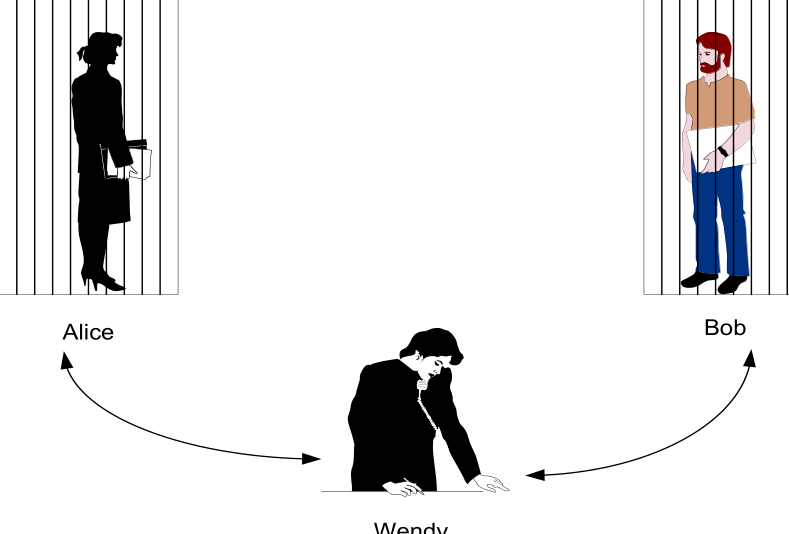
\includegraphics[width=86.31mm,height=146.72mm]{images/llm/page_002_img_01.png}%
\end{textblock*}

\newpage

% --- unit llm 3 ---
% === Halaman 3 (llm) ===

\begin{itemize}
    \item Bagaimana cara Bob mengirim pesan rahasia kepada Alice tanpa diketahui oleh Wendy?
    \item Alternatif 1: mengenkripsinya
\end{itemize}

\vspace{5mm}

\textcolor{red}{xjT\#9uvmY!rc\$7yt59hth@\#}

\vspace{5mm}

\textit{Wendy pasti curiga!}

\newpage

% --- unit llm 4 ---
% === Halaman 4 (llm) ===

\begin{itemize}
  \item Alternatif 2: menyembunyikannya di dalam tulisan lain
\end{itemize}

\textcolor{blue}{masihkah} \textcolor{blue}{ada} \textcolor{blue}{lara} \textcolor{blue}{apabila} \textcolor{blue}{memoriku} \textcolor{red}{ingat} \textcolor{blue}{nestapa} \textcolor{blue}{itu.} \textcolor{red}{kita} \textcolor{red}{ingin} \textcolor{red}{tetap}
\textcolor{blue}{abadikan} \textcolor{blue}{kisah} \textcolor{blue}{asmara.} \textcolor{red}{bersamamu} \textcolor{blue}{usiaku} \textcolor{red}{renta.}

\vspace{5mm}

Wendy tidak akan curiga!

\vspace{5mm}

Information hiding dengan steganografi!

\newpage

% --- unit llm 5 ---
% === Halaman 5 (llm) ===

\section*{Apa Steganografi itu?}

\begin{itemize}
    \item Dari Bahasa Yunani: \textit{steganos} + \textit{graphien}
    \begin{itemize}
        \item \textcolor{red}{"steganos"} ($\sigma\tau\epsilon\gamma\alpha\nu\acute{o}\varsigma$): tersembunyi
        \item \textcolor{red}{"graphien"} ($\gamma\rho\alpha\phi\acute{\iota}\alpha$): tulisan
    \end{itemize}
    steganografi: tulisan tersembunyi (\textit{covered writing})
    
    \item \textbf{Steganography}: ilmu dan seni menyembunyikan pesan rahasia dengan suatu cara sedemikian sehingga tidak seorang pun yang mencurigai keberadaan pesan tersebut.
\end{itemize}

Tujuan steganografi: pesan tidak terdeteksi keberadaannya

\newpage

% --- unit llm 6 ---
% === Halaman 6 (llm) ===

\section*{Perbedaan Kriptografi dan Steganografi}

\begin{itemize}
    \item \textbf{Kriptografi}: menyembunyikan \textit{makna} atau isi (\textit{content}) pesan
    $\rightarrow$ Tujuan: agar pesan tidak dapat dibaca oleh pihak ketiga (lawan)
    
    \item \textbf{Steganografi}: menyembunyikan \textit{keberadaan} (\textit{existence}) pesan
    $\rightarrow$ Tujuan: untuk menghindari kecurigaan (\textit{conspicuous}) dari pihak ketiga (lawan)
\end{itemize}

\newpage

% --- unit llm 7 ---
% === Halaman 7 (llm) ===

\begin{center}
\Huge Kriptografi
\end{center}

\vspace{60mm}

\begin{center}
\color{red} Pesan yang dienkripsi dengan kriptografi menimbulkan kecurigaan bagi pengamat. \\
\color{red} Cipherteks dapat dideteksi keberadaannya.
\end{center}

% deskripsi: Ilustrasi konsep kriptografi yang menunjukkan pengirim, penerima, pesan terenkripsi berupa simbol acak (@2*\$#d(*%7*), dan pengamat yang menggunakan kaca pembesar untuk menyelidiki pesan tersebut.
% bbox normalisasi: [0.1870, 0.2130, 0.8140, 0.7430]
\begin{textblock*}{131.67mm}(39.27mm,63.26mm)
\noindent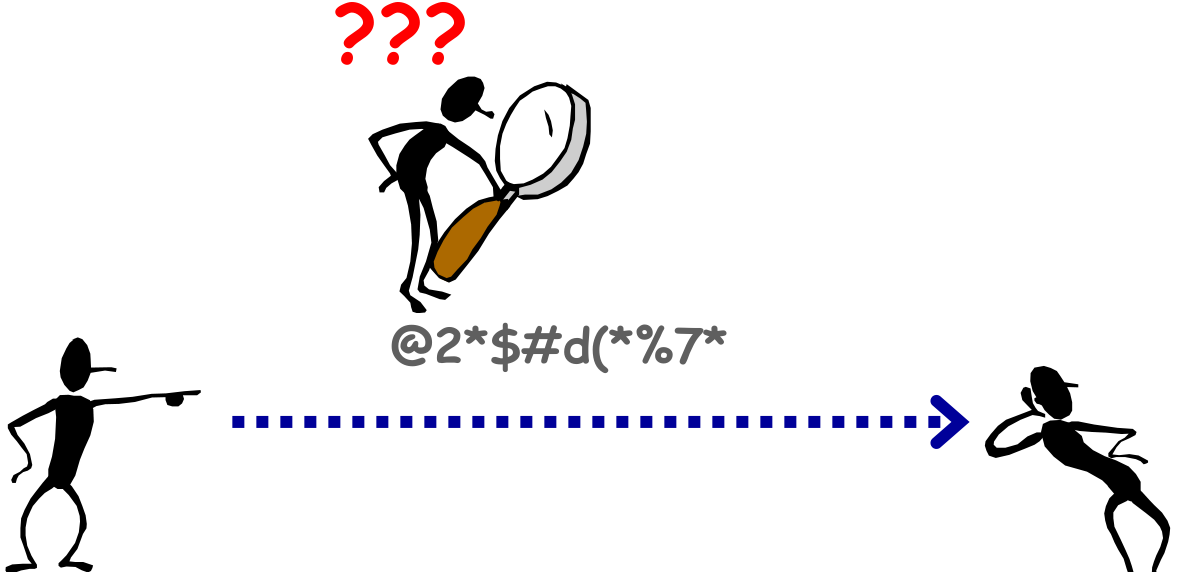
\includegraphics[width=131.67mm,height=157.41mm]{images/llm/page_007_img_01.png}%
\end{textblock*}

\newpage

% --- unit llm 8 ---
% === Halaman 8 (llm) ===

\vspace{127.71mm}

Kriptografi mengenkripsi pesan sehingga maknanya tersamar
\vspace{20mm}

% deskripsi: Diagram proses enkripsi dan dekripsi yang menunjukkan perubahan dari plaintext 'Keamanan informasi' menjadi ciphertext '%j&g+9*4$\$jd8)?hyt8' melalui proses Enkripsi, dan sebaliknya melalui proses Dekripsi.
% bbox normalisasi: [0.1500, 0.2800, 0.8500, 0.7100]
\begin{textblock*}{147.00mm}(31.50mm,83.16mm)
\noindent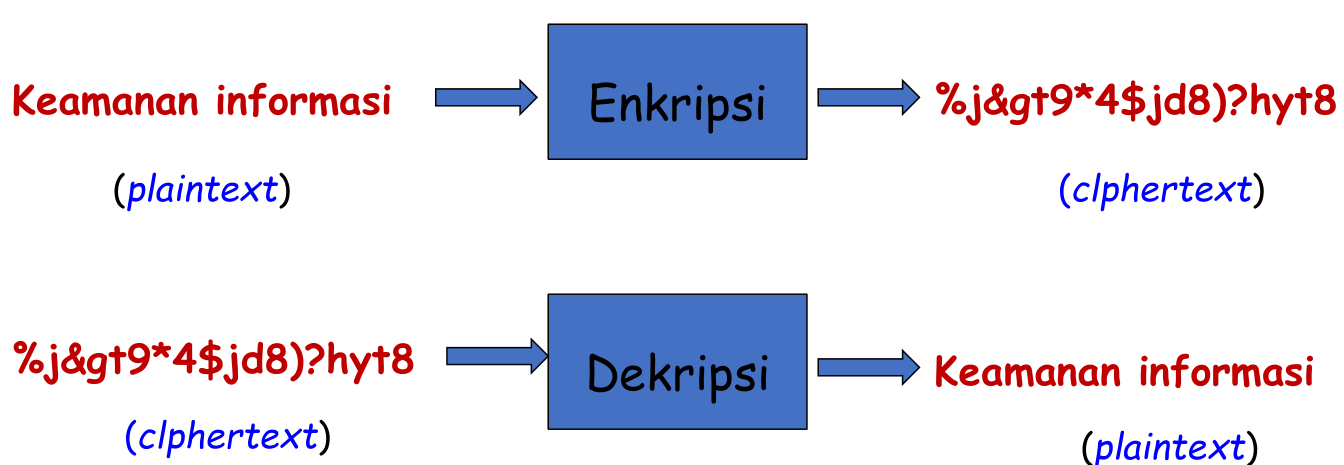
\includegraphics[width=147.00mm,height=127.71mm]{images/llm/page_008_img_01.png}%
\end{textblock*}

\newpage

% --- unit llm 9 ---
% === Halaman 9 (llm) ===

\begin{center}
\Huge Steganografi
\end{center}

\vspace{60mm}

\begin{center}
\textcolor{red}{\large Stego-data tidak menimbulkan kecurigaan bagi pengamat \\
 Pesan yang tersembunyi di dalamnya tidak dapat dideteksi.}
\end{center}

% deskripsi: Ilustrasi konsep steganografi yang menunjukkan proses pengiriman pesan tersembunyi antara dua orang, dengan seorang pengamat yang menggunakan kaca pembesar namun tidak dapat mendeteksi pesan tersebut.
% bbox normalisasi: [0.1800, 0.2200, 0.8200, 0.7400]
\begin{textblock*}{134.40mm}(37.80mm,65.34mm)
\noindent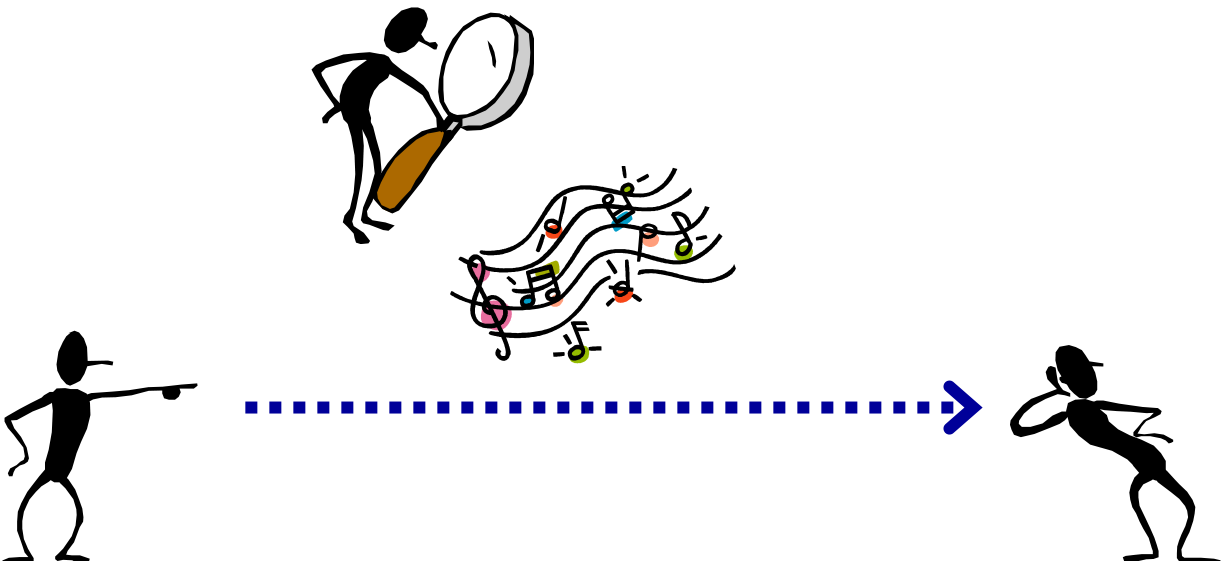
\includegraphics[width=134.40mm,height=154.44mm]{images/llm/page_009_img_01.png}%
\end{textblock*}

\newpage

% --- unit llm 10 ---
% === Halaman 10 (llm) ===

Steganografi menyembunyikan eksistensi pesan sehingga keberadaannya tidak diketahui

\vspace{10mm}

\textcolor{red}{\textbf{Keamanan informasi}}

% deskripsi: Foto berbagai macam paprika berwarna hijau, kuning, dan merah yang digunakan sebagai ilustrasi konsep steganografi (menyembunyikan pesan dalam media gambar).
% bbox normalisasi: [0.4650, 0.1930, 0.8970, 0.8060]
\begin{textblock*}{90.72mm}(97.65mm,57.32mm)
\noindent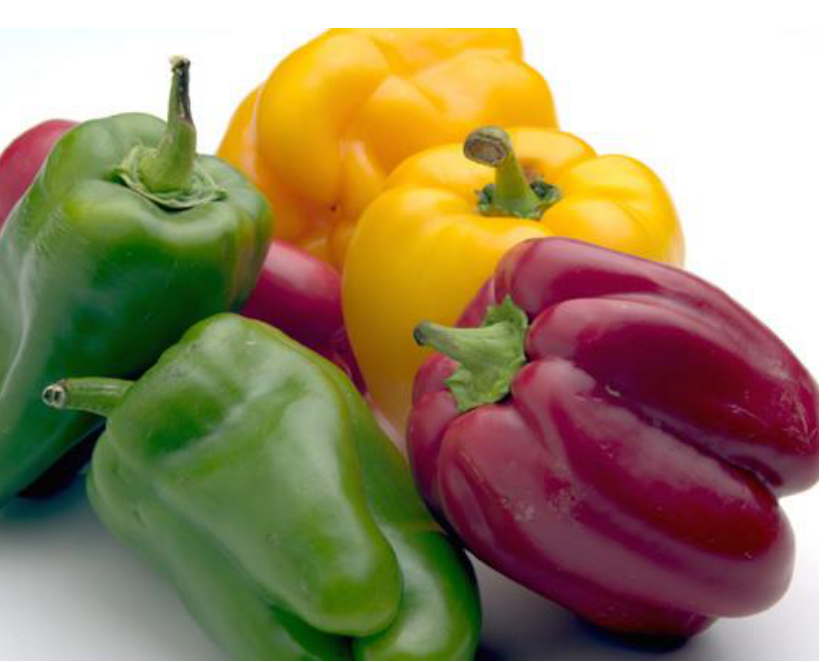
\includegraphics[width=90.72mm,height=182.06mm]{images/llm/page_010_img_01.png}%
\end{textblock*}

\newpage

% --- unit llm 11 ---
% === Halaman 11 (llm) ===

\section*{Sejarah Steganografi}

\begin{itemize}
    \item Usia steganografi setua usia kriptografi, dan sejarah keduanya berjalan bersamaan.
\end{itemize}

\begin{itemize}
    \item Periode sejarah steganografi dapat dibagi menjadi:
    \begin{enumerate}
        \item Steganografi kuno (\textit{ancient steganography})
        \item Steganografi zaman renaisans (\textit{renaissance steganography})
        \item Steganografi zaman perang dunia
        \item Steganografi modern
    \end{enumerate}
\end{itemize}

\newpage

% --- unit llm 12 ---
% === Halaman 12 (llm) ===

\vspace{68.31mm}

\section*{Ancient Steganography}

\begin{itemize}
    \item \textbf{Steganografi dengan media kepala budak.}
\end{itemize}

Ditulis oleh Herodotus ($485 - 525$ BC), sejarawan Yunani pada tahun $440$ BC di dalam buku: \textit{Histories of Herodotus}. Kisah perang antara kerajaan Persia dan rakyat Yunani.

\vspace{10mm}

Herodotus menceritakan cara \textbf{Histaiaeus} mengirim pesan kepada \textbf{Aristagoras of Miletus} untuk melawan Persia. Caranya: Dipilih beberapa budak. Kepala budak dibotaki, ditulisi pesan dengan cara tato, rambut budak dibiarkan tumbuh, budak dikirim. Di tempat penerima kepala budak digunduli agar pesan bisa dibaca.

% deskripsi: Potret Herodotus
% bbox normalisasi: [0.8800, 0.0100, 0.9770, 0.2400]
\begin{textblock*}{20.37mm}(184.80mm,2.97mm)
\noindent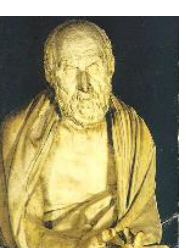
\includegraphics[width=20.37mm,height=68.31mm]{images/llm/page_012_img_01.png}%
\end{textblock*}

% deskripsi: Ilustrasi proses steganografi pada kepala: tato pesan, penumbuhan rambut, dan pencukuran kembali untuk membaca pesan
% bbox normalisasi: [0.1600, 0.7000, 0.8500, 0.9500]
\begin{textblock*}{144.90mm}(33.60mm,207.90mm)
\noindent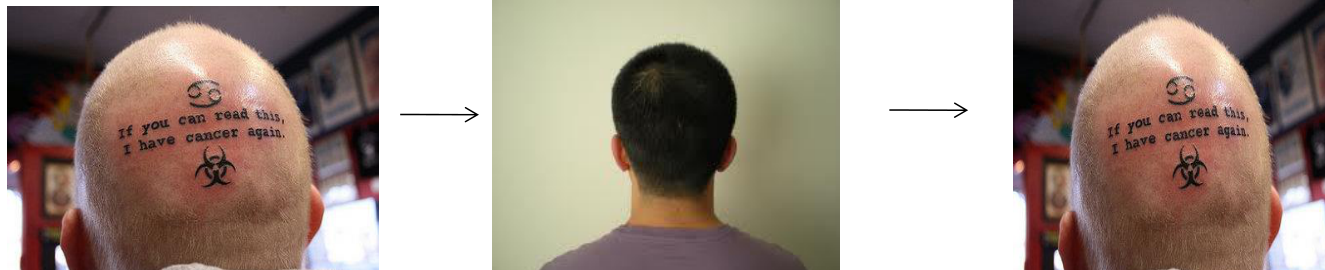
\includegraphics[width=144.90mm,height=74.25mm]{images/llm/page_012_img_02.png}%
\end{textblock*}

\newpage

% --- unit llm 13 ---
% === Halaman 13 (llm) ===

\begin{itemize}
  \item \textbf{Penggunaan \textit{tablet wax}}

  Orang-orang Yunani kuno menulis pesan rahasia di atas kayu yang kemudian ditutup dengan lilin (\textit{wax}).
\end{itemize}

\vspace{10mm}

Di dalam bukunya, Heradatus menceritakan Demaratus mengirim peringatan tentang serangan yang akan datang ke Yunani dengan menulis langsung pada tablet kayu yang kemudian dilapisi lilin dari lebah.

% deskripsi: Ilustrasi tablet lilin (wax tablet) kuno yang terdiri dari dua papan kayu dengan lapisan lilin gelap di dalamnya dan alat tulis kayu (stylus).
% bbox normalisasi: [0.2930, 0.5550, 0.6750, 0.9050]
\begin{textblock*}{80.22mm}(61.53mm,164.84mm)
\noindent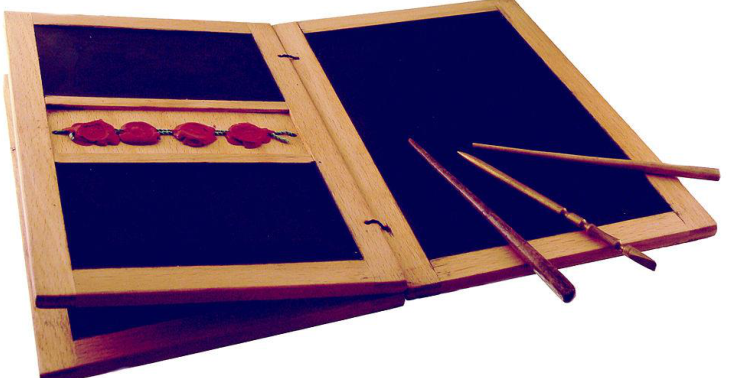
\includegraphics[width=80.22mm,height=103.95mm]{images/llm/page_013_img_01.png}%
\end{textblock*}

\newpage

% --- unit llm 14 ---
% === Halaman 14 (llm) ===

\begin{itemize}
    \item Penggunaan tinta tak-tampak (\textit{invisible ink})
\end{itemize}

\vspace{10mm}

Pliny the Elder menjelaskan penggunaan tinta dari getah tanaman \textit{thithymallus}. Jika dituliskan pada kertas maka tulisan dengan tinta tersebut tidak kelihatan, tetapi bila kertas dipanaskan berubah menjadi gelap/coklat

\vspace{5mm}

Pliny the Elder.
AD 23 - 79

% deskripsi: Ilustrasi gambar kuno tokoh Pliny the Elder
% bbox normalisasi: [0.1100, 0.2780, 0.2650, 0.6600]
\begin{textblock*}{32.55mm}(23.10mm,82.57mm)
\noindent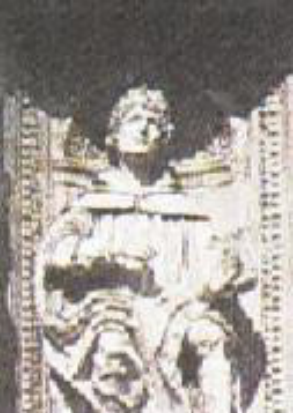
\includegraphics[width=32.55mm,height=113.45mm]{images/llm/page_014_img_01.png}%
\end{textblock*}

\newpage

% --- unit llm 15 ---
% === Halaman 15 (llm) ===

\textbf{Penggunaan kain sutra dan lilin}

\vspace{121.77mm}

\begin{itemize}
    \item Orang Cina kuno menulis catatan pada potongan-potongan kecil sutra yang kemudian digumpalkan menjadi bola kecil dan dilapisi lilin.
    \vspace{20mm}
    \item Selanjutnya bola kecil tersebut ditelan oleh si pembawa pesan.
    \item Pesan dibaca setelah bola kecil dikeluarkan dari perut si pembawa pesan dengan cara BAB.
\end{itemize}

% deskripsi: Ilustrasi kartun seekor panda yang sedang memegang daun hijau.
% bbox normalisasi: [0.7100, 0.3300, 0.8900, 0.7400]
\begin{textblock*}{37.80mm}(149.10mm,98.01mm)
\noindent
\includegraphics[width=37.80mm,height=121.77mm]{images/llm/page_015_img_01.png}%
\end{textblock*}

\newpage

% --- unit llm 16 ---
% === Halaman 16 (llm) ===

\section*{Renaissance Steganography}

\vspace{10mm}

Tahun 1499, Johannes Trithemius menulis buku \textbf{Steganographia}, yang menceritakan tentang metode steganografi berbasis karakter

\vspace{10mm}

Johannes Trithemius \\ (1404--1472 )

\vspace{10mm}

Selanjutnya tahun 1518 dia menulis buku tentang steganografi dan kriptografi, berjudul \textbf{Polygraphiae}.

% deskripsi: Potret Johannes Trithemius
% bbox normalisasi: [0.0700, 0.0900, 0.2500, 0.4400]
\begin{textblock*}{37.80mm}(14.70mm,26.73mm)
\noindent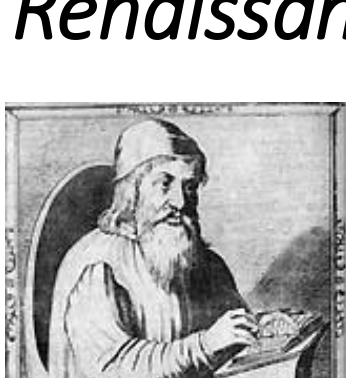
\includegraphics[width=37.80mm,height=103.95mm]{images/llm/page_016_img_01.png}%
\end{textblock*}

% deskripsi: Halaman judul buku Steganographia
% bbox normalisasi: [0.2800, 0.2000, 0.6400, 0.7700]
\begin{textblock*}{75.60mm}(58.80mm,59.40mm)
\noindent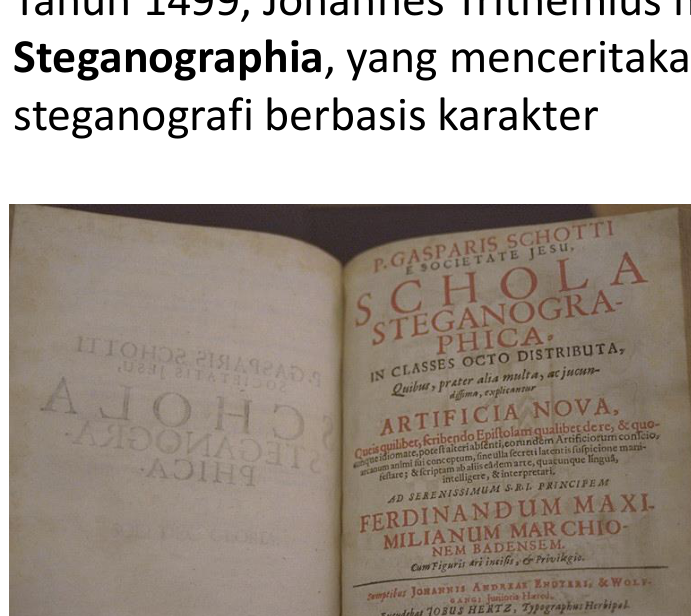
\includegraphics[width=75.60mm,height=169.29mm]{images/llm/page_016_img_02.png}%
\end{textblock*}

% deskripsi: Halaman judul buku Polygraphiae
% bbox normalisasi: [0.6900, 0.2000, 0.8700, 0.6500]
\begin{textblock*}{37.80mm}(144.90mm,59.40mm)
\noindent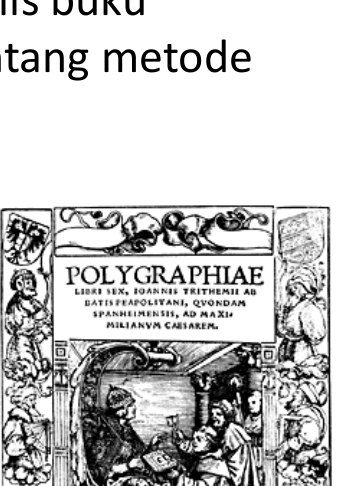
\includegraphics[width=37.80mm,height=133.65mm]{images/llm/page_016_img_03.png}%
\end{textblock*}

\newpage

% --- unit llm 17 ---
% === Halaman 17 (llm) ===

\vspace{162.16mm}

Giovanni Battista Porta menggambarkan cara menyembunyikan pesan di dalam telur rebus.\\
\nCaranya, pesan ditulis pada kulit telur yang dibuat dari tinta khusus yang dibuat dengan satu ons tawas dan setengah liter cuka.\\
\nPrinsipnya penyembunyiannya adalah tinta tersebut akan menembus kulit telur yang berpori, tanpa meninggalkan jejak yang terlihat.\\
\vspace{10mm}
Giovanni Battista Porta \\ (1535-1615) \\
\vspace{5mm}
Tulisan dari tinta akan membekas pada permukaan isi telur yang telah mengeras (karena sudah direbus sebelumnya). Pesan dibaca dengan membuang kulit telur

% deskripsi: Potret ilustrasi Giovanni Battista Porta dalam bingkai oval.
% bbox normalisasi: [0.0840, 0.0900, 0.3700, 0.6360]
\begin{textblock*}{60.06mm}(17.64mm,26.73mm)
\noindent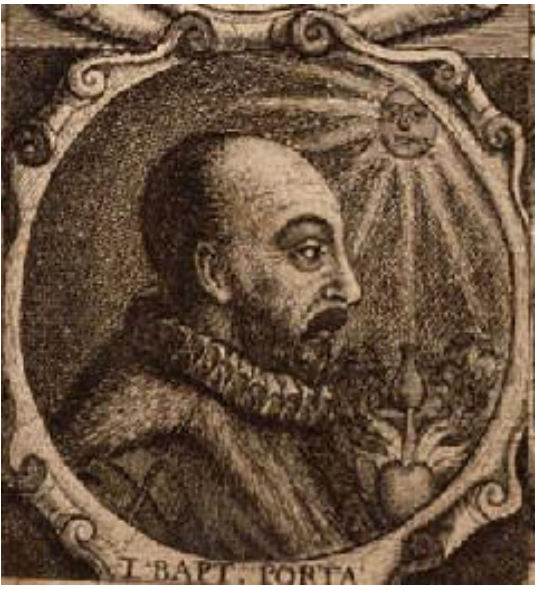
\includegraphics[width=60.06mm,height=162.16mm]{images/llm/page_017_img_01.png}%
\end{textblock*}

\newpage

% --- unit llm 18 ---
% === Halaman 18 (llm) ===

\section*{World War Steganography}

\begin{itemize}
    \item Penggunaan tinta tak-tampak (\textit{invisible ink}) dalam spionase.
    \begin{itemize}
        \item Pada Perang Dunia II, tinta tak-tampak digunakan untuk menulis pesan rahasia
        \item Tinta terbuat dari campuran susu, sari buah, cuka, dan urine.
        \item Cara membaca: Kertas dipanaskan sehingga tulisan dari tinta tak-tampak tersebut akan menghitam.
    \end{itemize}
\end{itemize}

\vspace{10mm}

Seorang agen FBI sedan menggunakan sinar ultraviolet untuk membaca tulisan yang tersembunyi pada kertas yang dicurigai dari agen spionase.

% deskripsi: Foto hitam putih seorang agen FBI yang sedang menggunakan alat sinar ultraviolet untuk mendeteksi tulisan tersembunyi pada selembar kertas.
% bbox normalisasi: [0.1240, 0.5080, 0.4070, 0.8930]
\begin{textblock*}{59.43mm}(26.04mm,150.88mm)
\noindent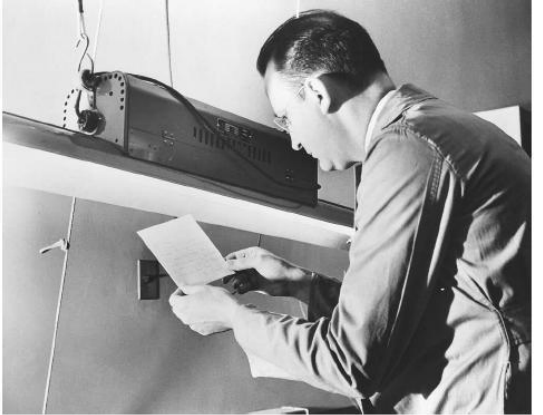
\includegraphics[width=59.43mm,height=114.34mm]{images/llm/page_018_img_01.png}%
\end{textblock*}

\newpage

% --- unit llm 19 ---
% === Halaman 19 (llm) ===

\begin{itemize}
    \item \textbf{Steganografi dalam Perang Dunia II: \textit{Null Cipher}}
\end{itemize}

Pesan berikut dikirim oleh Kedubes Jerman pada PD II:

\textcolor{red}{A}p\textcolor{red}{p}arently \textcolor{red}{n}eutral's \textcolor{red}{p}rotest \textcolor{red}{i}s \textcolor{red}{t}horoughly \textcolor{red}{d}iscounted \textcolor{red}{a}nd \textcolor{red}{i}gnored. \textcolor{red}{S}man \textcolor{red}{h}ard \textcolor{red}{i}t. \textcolor{red}{B}lockade \textcolor{red}{l}ssue \textcolor{red}{a}ffects \textcolor{red}{p}retext \textcolor{red}{f}or \textcolor{red}{e}mbargo \textcolor{red}{o}n \textcolor{red}{b}y-\textcolor{red}{p}roducts, \textcolor{red}{e}jecting \textcolor{red}{s}uets \textcolor{red}{a}nd \textcolor{red}{v}egetable \textcolor{red}{o}ils.

Ambil huruf kedua setiap kata, diperoleh pesan berikut: \textcolor{red}{Pershing sails from NY June 1}.

\newpage

% --- unit llm 20 ---
% === Halaman 20 (llm) ===

Contoh \textit{Null Cipher} lainnya:

\textcolor{blue}{B}ig \textcolor{blue}{r}umble in \textcolor{blue}{N}ew \textcolor{blue}{G}uinea.\\
\textcolor{blue}{T}he \textcolor{blue}{w}ar \textcolor{blue}{o}n \textcolor{blue}{c}elebrity \textcolor{blue}{a}cts \textcolor{blue}{s}hould \textcolor{blue}{e}nd \textcolor{blue}{s}oon.\\
\textcolor{blue}{O}ver \textcolor{blue}{f}our \textcolor{blue}{d}ie \textcolor{blue}{e}cstatic \textcolor{blue}{e}lephants \textcolor{blue}{r}eplicated.

\vspace{5mm}

\textcolor{red}{Bring two cases of deer.}

\newpage

% --- unit llm 21 ---
% === Halaman 21 (llm) ===

Fishing freshwater bends and saltwater coasts rewards anyone\nfeeling stressed. Resourceful anglers usually find masterful leapers\nfun and admit swordfish rank overwhelming anyday.\n\nDengan mengambil huruf ketiga pada setiap kata diperoleh pesan\nberikut:\n\n\textcolor{red}{Send Lawyers, Guns, and Money.}

\newpage

% --- unit llm 22 ---
% === Halaman 22 (llm) ===

\begin{itemize}
  \item Steganografi di dalam film \textit{Mercury Rising} dan \textit{Beautiful Mind}
\end{itemize}

\vspace{10mm}

% deskripsi: Cuplikan layar dari film A Beautiful Mind yang menunjukkan karakter sedang berada di depan kaca dengan banyak coretan rumus matematika dan teks.
% bbox normalisasi: [0.1400, 0.2700, 0.4580, 0.8450]
\begin{textblock*}{66.78mm}(29.40mm,80.19mm)
\noindent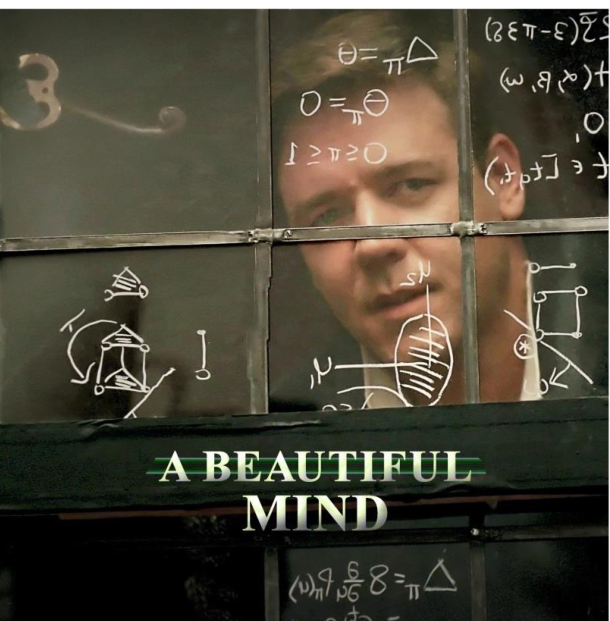
\includegraphics[width=66.78mm,height=170.77mm]{images/llm/page_022_img_01.png}%
\end{textblock*}

% deskripsi: Poster film Mercury Rising yang menampilkan Bruce Willis dan seorang anak kecil.
% bbox normalisasi: [0.5550, 0.2700, 0.7810, 0.8500]
\begin{textblock*}{47.46mm}(116.55mm,80.19mm)
\noindent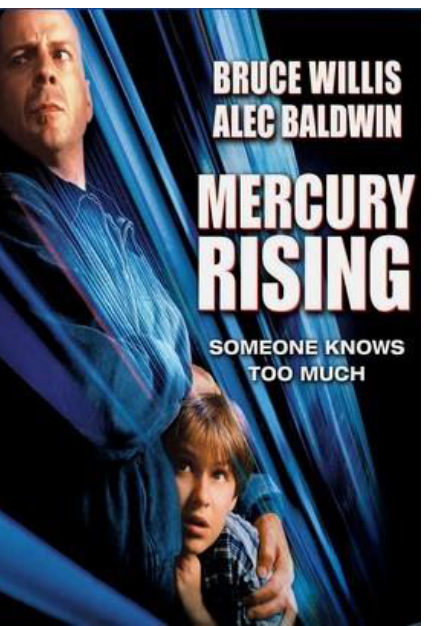
\includegraphics[width=47.46mm,height=172.26mm]{images/llm/page_022_img_02.png}%
\end{textblock*}

\newpage

% --- unit llm 23 ---
% === Halaman 23 (llm) ===

\vspace{132.16mm}

Beberapa adegan film \textit{Beautiful Mind} yang memperlihatkan steganografi

\vspace{130.68mm}

% deskripsi: Screenshot adegan film A Beautiful Mind yang menunjukkan layar dengan banyak teks dan kode, dengan subtitle 'Ever just know something, Dr. Nash?'
% bbox normalisasi: [0.1180, 0.0530, 0.5200, 0.4980]
\begin{textblock*}{84.42mm}(24.78mm,15.74mm)
\noindent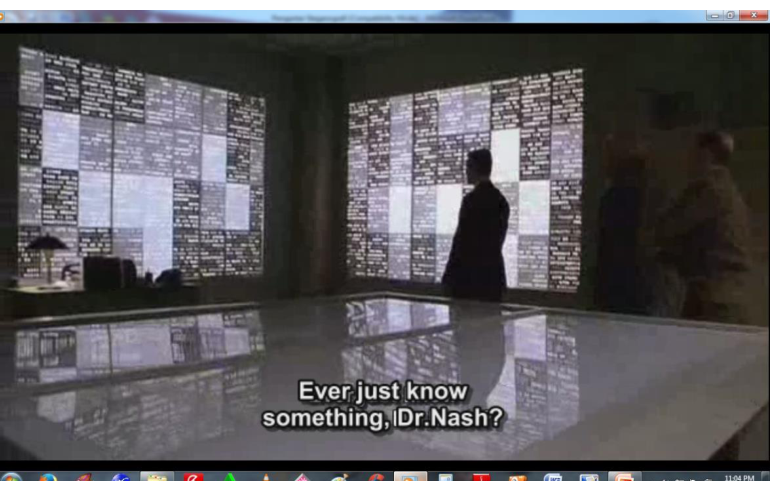
\includegraphics[width=84.42mm,height=132.16mm]{images/llm/page_023_img_01.png}%
\end{textblock*}

% deskripsi: Screenshot adegan film A Beautiful Mind yang menunjukkan teks 'ARTIFICIAL LIFE' dalam sebuah dokumen.
% bbox normalisasi: [0.4610, 0.5280, 0.8830, 0.9680]
\begin{textblock*}{88.62mm}(96.81mm,156.82mm)
\noindent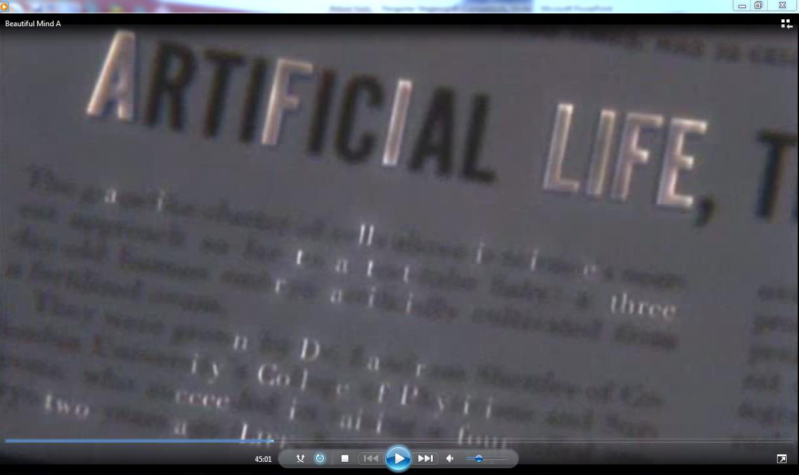
\includegraphics[width=88.62mm,height=130.68mm]{images/llm/page_023_img_02.png}%
\end{textblock*}

\newpage

% --- unit llm 24 ---
% === Halaman 24 (llm) ===

\section*{Steganografi dan Terorisme}

\begin{itemize}
    \item Ilmu steganografi mendadak naik daun ketika pasca 11 September 2001 pihak FBI menuding Al-Qaidah menggunakan steganografi untuk menyisipkan pesan rahasia melalui video atau gambar yang mereka rilis secara teratur di Internet.
\end{itemize}

\vspace{10mm}

% deskripsi: Foto gedung World Trade Center yang terbakar setelah serangan 11 September.
% bbox normalisasi: [0.1380, 0.5010, 0.4140, 0.8860]
\begin{textblock*}{57.96mm}(28.98mm,148.80mm)
\noindent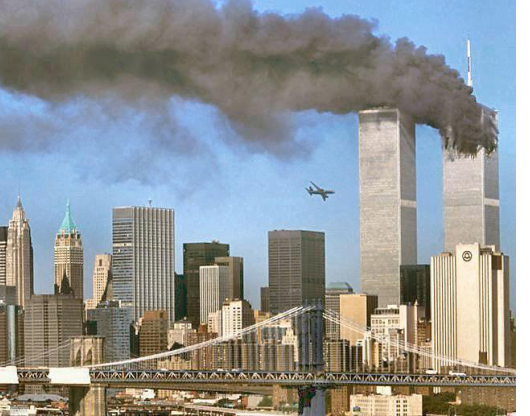
\includegraphics[width=57.96mm,height=114.34mm]{images/llm/page_024_img_01.png}%
\end{textblock*}

% deskripsi: Screenshot cuplikan video yang menampilkan teks Arab dan bendera Al-Qaeda.
% bbox normalisasi: [0.5360, 0.5010, 0.7630, 0.8930]
\begin{textblock*}{47.67mm}(112.56mm,148.80mm)
\noindent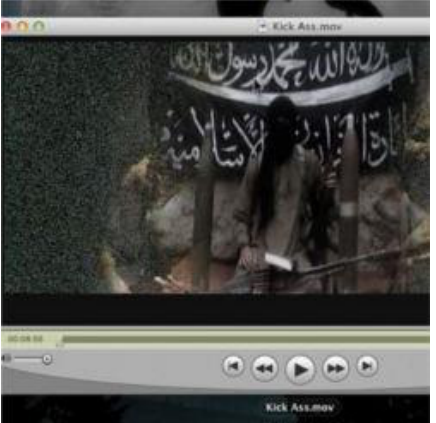
\includegraphics[width=47.67mm,height=116.42mm]{images/llm/page_024_img_02.png}%
\end{textblock*}

\newpage

% --- unit llm 25 ---
% === Halaman 25 (llm) ===

\section*{Steganografi Digital}

\begin{itemize}
    \item Steganografi digital: penyembunyian pesan digital di dalam dokumen digital lainnya.
    \item \textit{Carrier file}: dokumen digital yang digunakan sebagai media untuk menyembunyikan pesan.
\end{itemize}

\vspace{53.46mm}

\begin{enumerate}
    \item Teks
    
    \textcolor{red}{"Kita semua bersaudara"}
    
    \begin{itemize}
        \item -Txt
        \item - doc
        \item - html
    \end{itemize}
    
    \vspace{10mm}
    
    \item Audio
    
    \vspace{5mm}
    
    \begin{itemize}
        \item - wav
        \item - mp3
    \end{itemize}

\vspace{18.71mm}

    \item Gambar (\textit{image})
    
    \begin{itemize}
        \item - bmp
        \item - jpeg
        \item - gif
        \item - png
    \end{itemize}
    
    \vspace{10mm}
    
    \item Video
    
    \begin{itemize}
        \item -mpeg
        \item - avi
        \item - mp4
    \end{itemize}
\end{enumerate}

% deskripsi: Gambar contoh file gambar berupa paprika warna-warni
% bbox normalisasi: [0.5580, 0.4900, 0.6620, 0.6700]
\begin{textblock*}{21.84mm}(117.18mm,145.53mm)
\noindent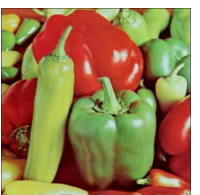
\includegraphics[width=21.84mm,height=53.46mm]{images/llm/page_025_img_01.png}%
\end{textblock*}

% deskripsi: Grafik bentuk gelombang audio
% bbox normalisasi: [0.1500, 0.8310, 0.4400, 0.8940]
\begin{textblock*}{60.90mm}(31.50mm,246.81mm)
\noindent
\includegraphics[width=60.90mm,height=18.71mm]{images/llm/page_025_img_02.png}%
\end{textblock*}

% deskripsi: Screenshot contoh file video yang menampilkan dua orang pria
% bbox normalisasi: [0.5500, 0.7630, 0.7760, 0.9250]
\begin{textblock*}{47.46mm}(115.50mm,226.61mm)
\noindent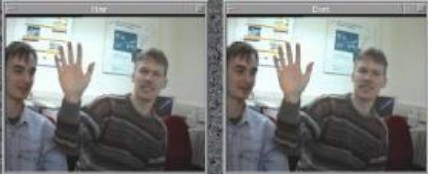
\includegraphics[width=47.46mm,height=48.11mm]{images/llm/page_025_img_03.png}%
\end{textblock*}

\newpage

% --- unit llm 26 ---
% === Halaman 26 (llm) ===

\vspace{210.87mm}

Carrier File \vspace{10mm} Carrier File with Hidden Message

% deskripsi: Ilustrasi konsep steganografi yang menunjukkan proses penyisipan pesan rahasia dari sebuah file teks ('myhiddenmessage.txt') ke dalam sebuah 'Carrier File' untuk menghasilkan 'Carrier File with Hidden Message'.
% bbox normalisasi: [0.1600, 0.1200, 0.8300, 0.8300]
\begin{textblock*}{140.70mm}(33.60mm,35.64mm)
\noindent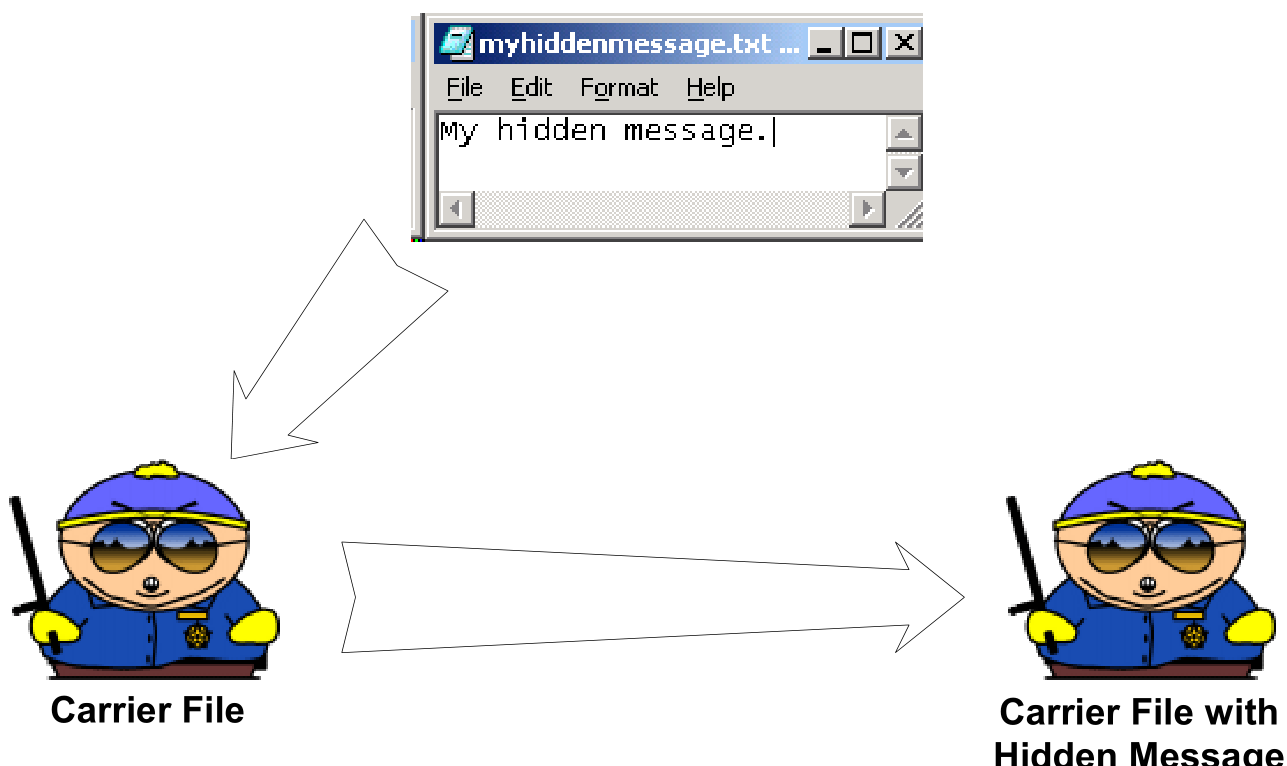
\includegraphics[width=140.70mm,height=210.87mm]{images/llm/page_026_img_01.png}%
\end{textblock*}

\newpage

% --- unit llm 27 ---
% === Halaman 27 (llm) ===

\section*{Terminologi Steganografi}

\begin{enumerate}
  \item \textit{Embedded message (hiddentext)} \textit{atau secret message}: pesan yang disembunyikan.
  
  Bisa berupa teks, gambar, audio, video, dll
  
  \item \textit{Cover-object (covertext)}: pesan yang digunakan untuk menyembunyikan \textit{embedded message}.
  
  Bisa berupa teks, gambar, audio, video, dll
  
  \item \textit{Stego-object (stegotext)}: pesan yang sudah berisi pesan \textit{embedded message}.
  
  \item \textit{Stego-key}: kunci yang digunakan untuk menyisipan pesan dan mengekstraksi pesan dari stegotext.
\end{enumerate}

\newpage

% --- unit llm 28 ---
% === Halaman 28 (llm) ===

\vspace{139.59mm}

\section*{Diagram Proses Steganografi}
\vspace{40mm}

% deskripsi: Diagram alur proses steganografi yang menunjukkan langkah-langkah dari pesan rahasia (Embedded message) yang digabungkan dengan cover-object menggunakan encoder dan kunci (key) untuk menghasilkan stego-object, yang kemudian didekode oleh decoder menggunakan kunci untuk mengekstraksi kembali pesan rahasia. Terdapat juga elemen 'adversary' yang mencoba menganalisis stego-object tersebut.
% bbox normalisasi: [0.1600, 0.3100, 0.8700, 0.7800]
\begin{textblock*}{149.10mm}(33.60mm,92.07mm)
\noindent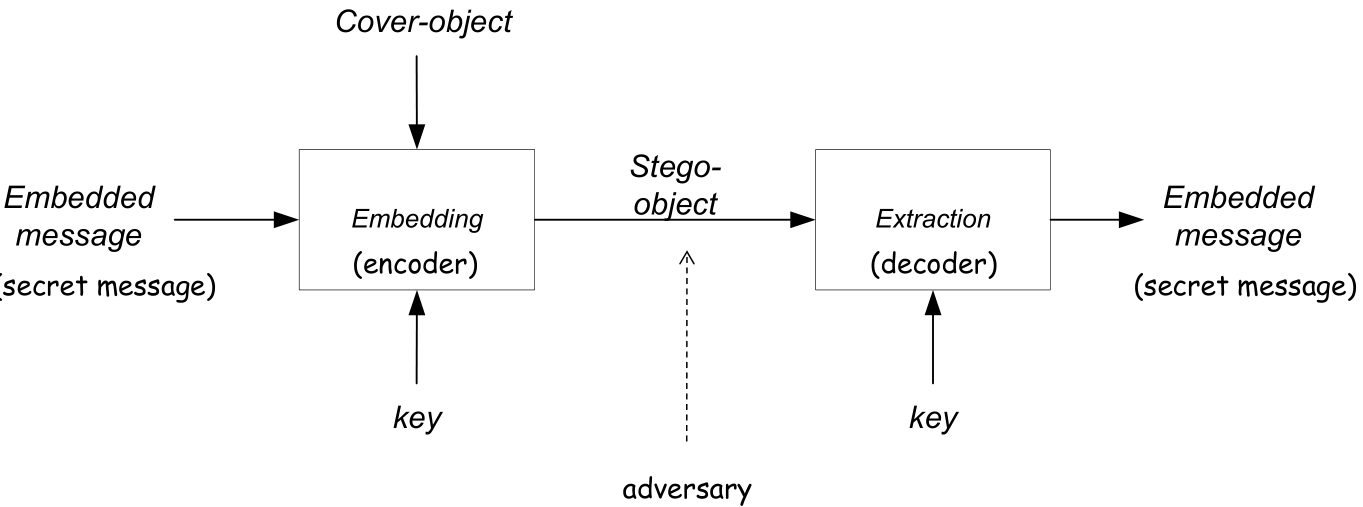
\includegraphics[width=149.10mm,height=139.59mm]{images/llm/page_028_img_01.png}%
\end{textblock*}

\newpage

% --- unit llm 29 ---
% === Halaman 29 (llm) ===

% (tidak ada teks dari model)

% deskripsi: Diagram alur proses steganografi yang menunjukkan proses embedding pada sisi pengirim (sender) menggunakan cover-object dan stego-key, pengiriman stego-object melalui jaringan (network), dan proses ekstraksi pada sisi penerima (receiver) untuk mendapatkan pesan yang disembunyikan (extracted message).
% bbox normalisasi: [0.0700, 0.2300, 0.9170, 0.8100]
\begin{textblock*}{177.87mm}(14.70mm,68.31mm)
\noindent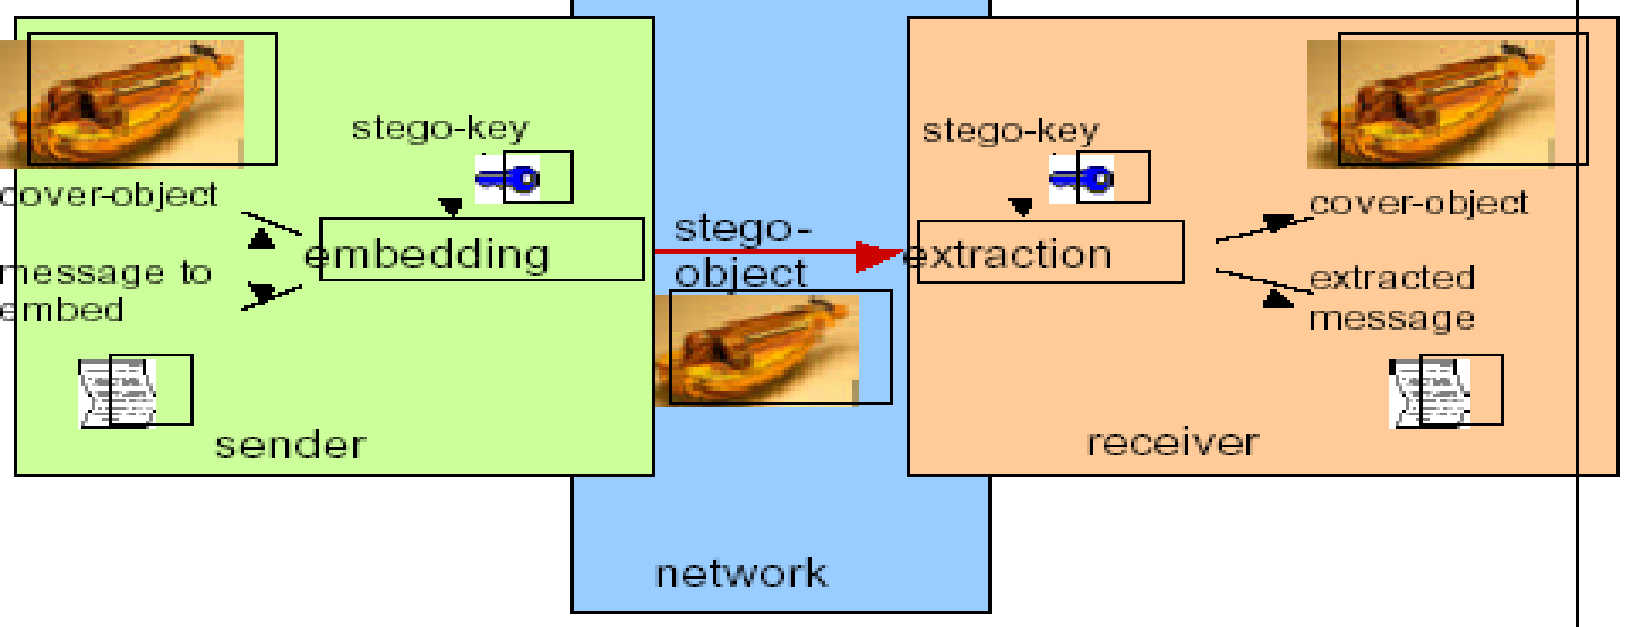
\includegraphics[width=177.87mm,height=172.26mm]{images/llm/page_029_img_01.png}%
\end{textblock*}

\newpage

% --- unit llm 30 ---
% === Halaman 30 (llm) ===

\vspace{137.21mm}

Istilah keilmuan serumpun terasa memberikan distorsi persepsi pada maksud sebenarnya. Persepsi yang segera terbentuk dengan istilah tesrebut adalah pertumbuhan dari akar-akar ilmu membentuk suatu rumpun, yang berarti bahwa nuansa historis organisasi/kelompok/unit yang mewadahinya.\\ \vspace{10mm} \begin{tabular}{ccc} Embedded message & Cover-image & Stego-image \end{tabular}

% deskripsi: Gambar cover-image yang menunjukkan sekumpulan paprika warna-warni.
% bbox normalisasi: [0.3340, 0.2120, 0.5880, 0.6740]
\begin{textblock*}{53.34mm}(70.14mm,62.96mm)
\noindent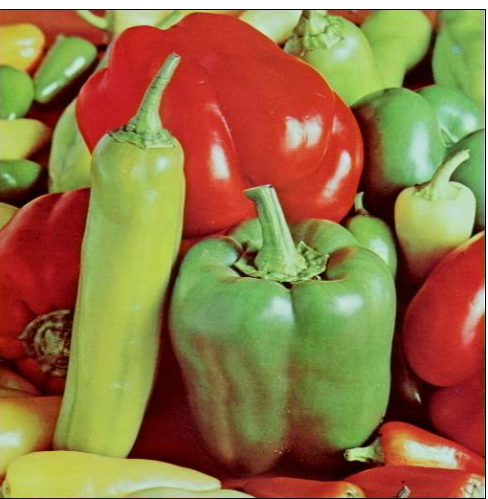
\includegraphics[width=53.34mm,height=137.21mm]{images/llm/page_030_img_01.png}%
\end{textblock*}

% deskripsi: Gambar stego-image yang terlihat identik dengan cover-image, digunakan untuk mengilustrasikan steganografi.
% bbox normalisasi: [0.6030, 0.2120, 0.8580, 0.6740]
\begin{textblock*}{53.55mm}(126.63mm,62.96mm)
\noindent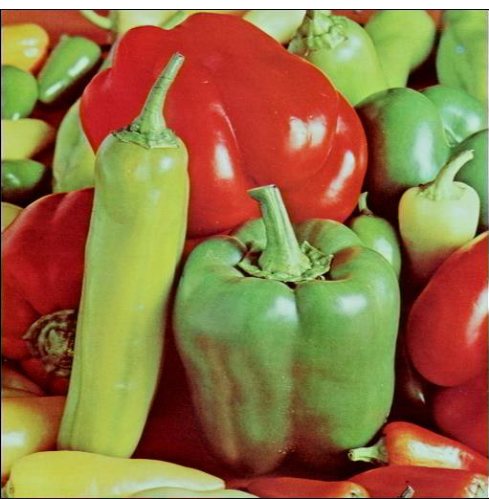
\includegraphics[width=53.55mm,height=137.21mm]{images/llm/page_030_img_02.png}%
\end{textblock*}

\newpage

% --- unit llm 31 ---
% === Halaman 31 (llm) ===

\begin{center}
\huge GIF image
\end{center}

\vspace{10mm}

\begin{center}
Cover image \quad Stego-image
\end{center}

\vspace{10mm}

\begin{center}
Embedded message
\end{center}

% deskripsi: Gambar cover yang menampilkan karakter Snow White dan para kurcaci.
% bbox normalisasi: [0.1920, 0.1230, 0.5040, 0.5320]
\begin{textblock*}{65.52mm}(40.32mm,36.53mm)
\noindent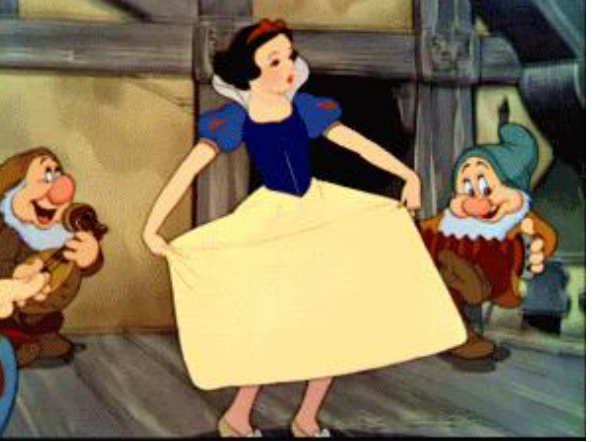
\includegraphics[width=65.52mm,height=121.47mm]{images/llm/page_031_img_01.png}%
\end{textblock*}

% deskripsi: Gambar stego-image yang terlihat identik dengan gambar cover, digunakan untuk menyembunyikan pesan.
% bbox normalisasi: [0.5430, 0.1230, 0.8550, 0.5320]
\begin{textblock*}{65.52mm}(114.03mm,36.53mm)
\noindent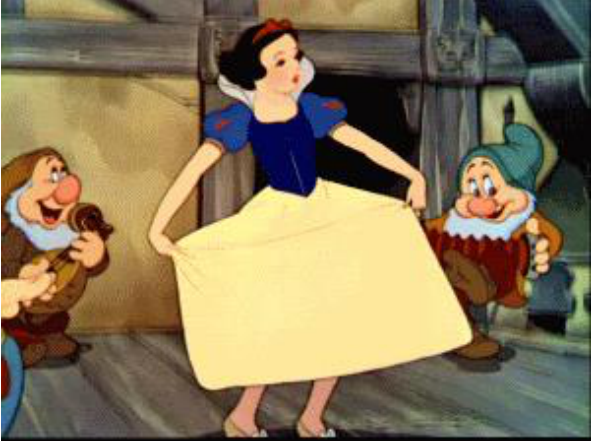
\includegraphics[width=65.52mm,height=121.47mm]{images/llm/page_031_img_02.png}%
\end{textblock*}

% deskripsi: Screenshot aplikasi Notepad yang berisi teks cerita Snow White sebagai pesan yang disembunyikan (embedded message).
% bbox normalisasi: [0.3770, 0.5960, 0.6650, 0.9070]
\begin{textblock*}{60.48mm}(79.17mm,177.01mm)
\noindent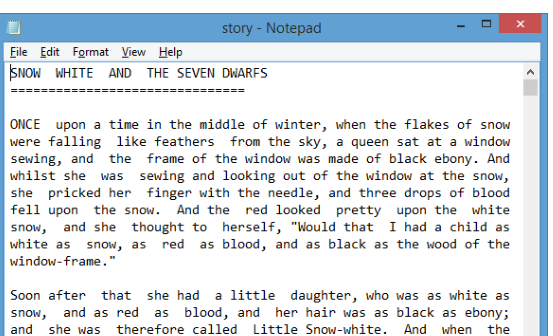
\includegraphics[width=60.48mm,height=92.37mm]{images/llm/page_031_img_03.png}%
\end{textblock*}

\newpage

% --- unit llm 32 ---
% === Halaman 32 (llm) ===

\vspace{114.05mm}

Cover image\vspace{10mm}
Stego-image

\vspace{114.05mm}

% deskripsi: Gambar asli (cover image) yang menampilkan seekor kucing Scottish Fold yang sedang dielus.
% bbox normalisasi: [0.1940, 0.0900, 0.5880, 0.4740]
\begin{textblock*}{82.74mm}(40.74mm,26.73mm)
\noindent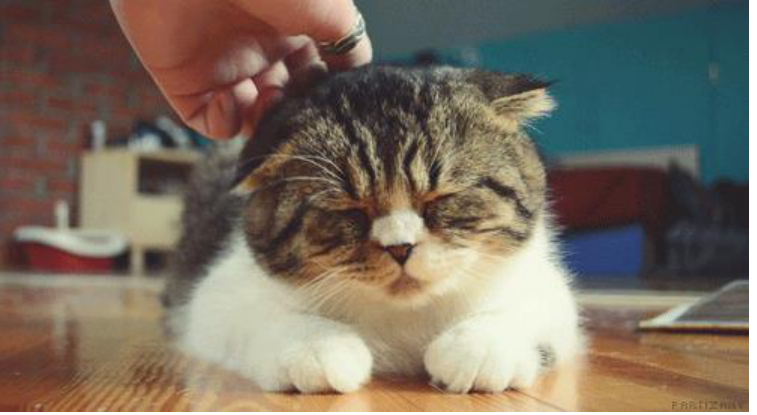
\includegraphics[width=82.74mm,height=114.05mm]{images/llm/page_032_img_01.png}%
\end{textblock*}

% deskripsi: Gambar stego (stego-image) yang secara visual tampak identik dengan cover image namun mengandung data tersembunyi.
% bbox normalisasi: [0.4380, 0.5260, 0.8320, 0.9100]
\begin{textblock*}{82.74mm}(91.98mm,156.22mm)
\noindent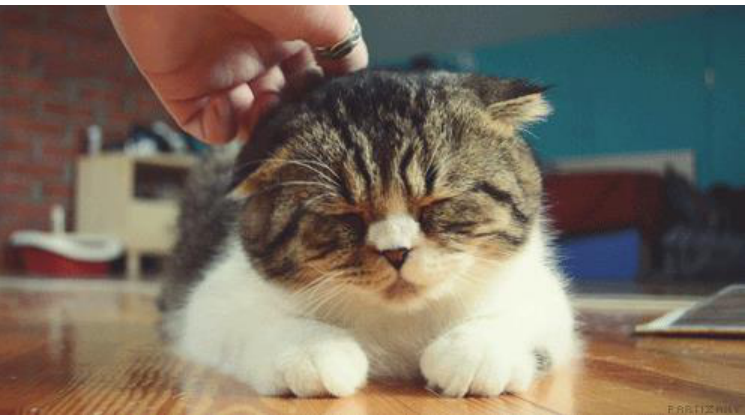
\includegraphics[width=82.74mm,height=114.05mm]{images/llm/page_032_img_02.png}%
\end{textblock*}

\newpage

% --- unit llm 33 ---
% === Halaman 33 (llm) ===

% (tidak ada teks dari model)

% deskripsi: Kolase gambar yang menunjukkan lukisan klasik suasana pesta atau kerumunan orang yang sebagian permukaannya tampak terkelupas atau terlipat, mengungkap latar belakang hitam putih yang abstrak di bawahnya.
% bbox normalisasi: [0.2600, 0.1500, 0.7670, 0.8030]
\begin{textblock*}{106.47mm}(54.60mm,44.55mm)
\noindent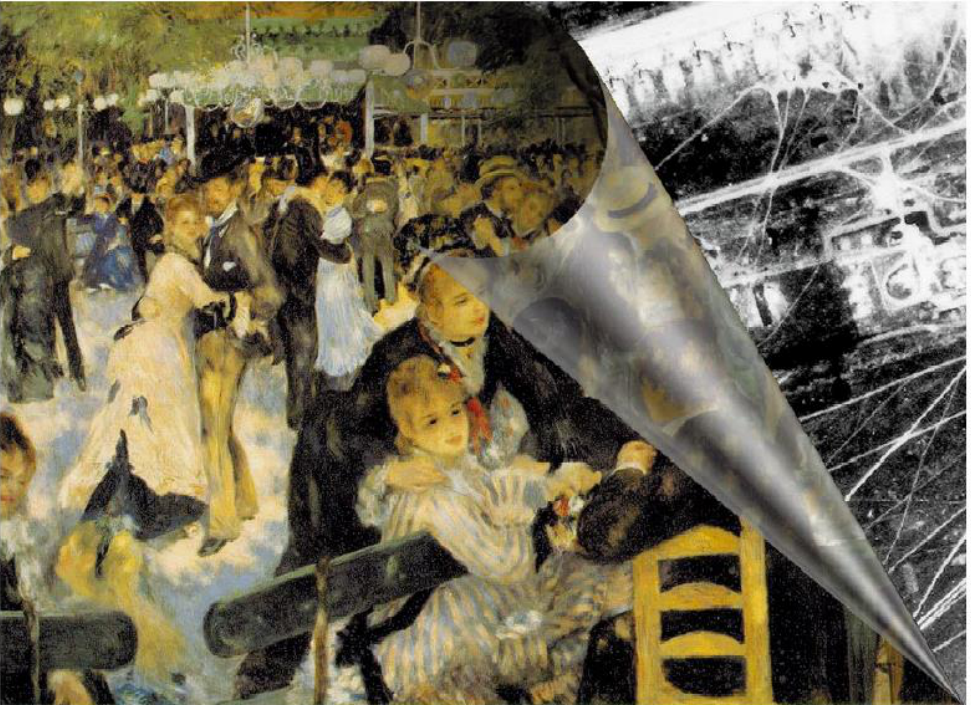
\includegraphics[width=106.47mm,height=193.94mm]{images/llm/page_033_img_01.png}%
\end{textblock*}

\newpage

% --- unit llm 34 ---
% === Halaman 34 (llm) ===

\vspace{147.01mm}

Cover image
\vspace{20mm}
Embedded image

\vspace{111.67mm}

% deskripsi: Gambar seekor hewan berwarna putih di atas salju yang digunakan sebagai contoh 'Cover image'.
% bbox normalisasi: [0.1520, 0.0260, 0.5550, 0.5210]
\begin{textblock*}{84.63mm}(31.92mm,7.72mm)
\noindent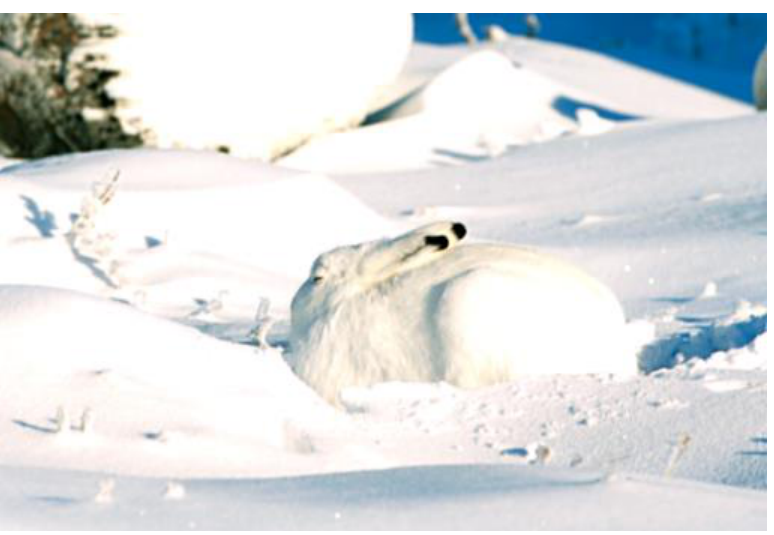
\includegraphics[width=84.63mm,height=147.01mm]{images/llm/page_034_img_01.png}%
\end{textblock*}

% deskripsi: Gambar sebuah pesawat jet tempur yang digunakan sebagai contoh 'Embedded image'.
% bbox normalisasi: [0.5190, 0.5280, 0.8330, 0.9040]
\begin{textblock*}{65.94mm}(108.99mm,156.82mm)
\noindent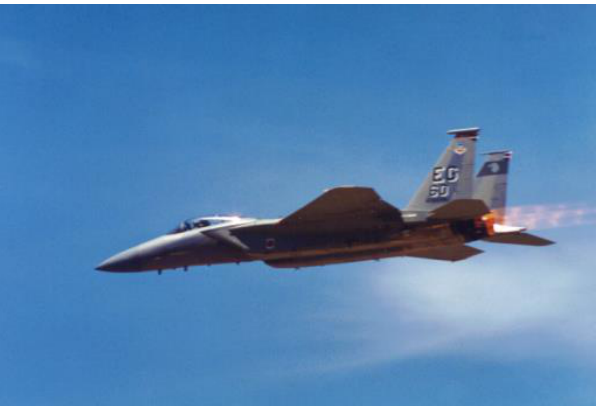
\includegraphics[width=65.94mm,height=111.67mm]{images/llm/page_034_img_02.png}%
\end{textblock*}

\newpage

% --- unit llm 35 ---
% === Halaman 35 (llm) ===

\vspace{145.53mm}

Stego-image
\vspace{20mm}
Extracted image

\vspace{109.89mm}

% deskripsi: Gambar stego yang menampilkan seekor rubah salju di tengah salju putih.
% bbox normalisasi: [0.1500, 0.0200, 0.5500, 0.5100]
\begin{textblock*}{84.00mm}(31.50mm,5.94mm)
\noindent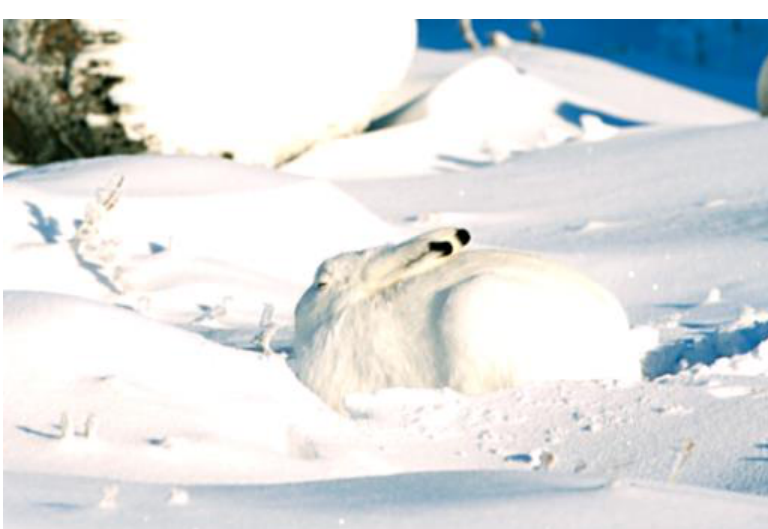
\includegraphics[width=84.00mm,height=145.53mm]{images/llm/page_035_img_01.png}%
\end{textblock*}

% deskripsi: Gambar yang diekstraksi menampilkan sebuah jet tempur yang sedang terbang.
% bbox normalisasi: [0.5100, 0.5300, 0.8300, 0.9000]
\begin{textblock*}{67.20mm}(107.10mm,157.41mm)
\noindent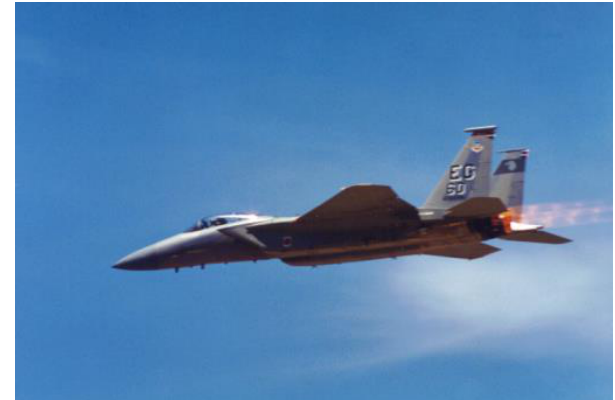
\includegraphics[width=67.20mm,height=109.89mm]{images/llm/page_035_img_02.png}%
\end{textblock*}

\newpage

% --- unit llm 36 ---
% === Halaman 36 (llm) ===

\section*{Kriteria Steganografi yang Bagus}

\begin{enumerate}
    \item \textcolor{red}{Imperceptible}\
    Keberadaan pesan rahasia tidak dapat dipersepsi secara visual atau secara audial
    \item \textcolor{red}{Fidelity.}\
    Kualitas \textit{cover-object} tidak jauh berubah akibat penyisipan pesan rahasia.
    \item \textcolor{red}{Recovery.}\
    Pesan yang disembunyikan harus dapat diekstraksi kembali.
    \item \textcolor{red}{Capacity}\
    Ukuran pesan yang disembunyikan sedapat mungkin besar
\end{enumerate}

\noindent Catatan: \textit{Robustnes} bukan isu penting di dalam steganografi

\newpage

% --- unit llm 37 ---
% === Halaman 37 (llm) ===

\section*{Kombinasi Kriptografi dan Steganografi}

\begin{itemize}
    \item Steganografi bukan pengganti kriptografi, tetapi keduanya saling melengkapi.
    \item Keamanan pesan rahasia dapat ditingkatkan dengan menggabungkan kriptografi dan steganografi.
    \item Mula-mula pesan dienkripsi dengan algoritma I kriptografi, selanjutnya pesan terenkripsi disembunyikan di dalam media lain (citra, video, audio, dll).
\end{itemize}

\newpage

% --- unit llm 38 ---
% === Halaman 38 (llm) ===

\vspace{199.58mm}

Steganography has its place in security. It is not intended to replace cryptography but supplement it. Hiding a message with steganography methods reduces the chance of a message being detected. However, if that message is also encrypted, if discovered, it must also be cracked (yet another layer of protection).

(David Kahn, penulis buku \textit{The Codebreakers - The Story of Secret Writing})

% deskripsi: Foto potret David Kahn, penulis buku The Codebreakers.
% bbox normalisasi: [0.6360, 0.1500, 0.9180, 0.8220]
\begin{textblock*}{59.22mm}(133.56mm,44.55mm)
\noindent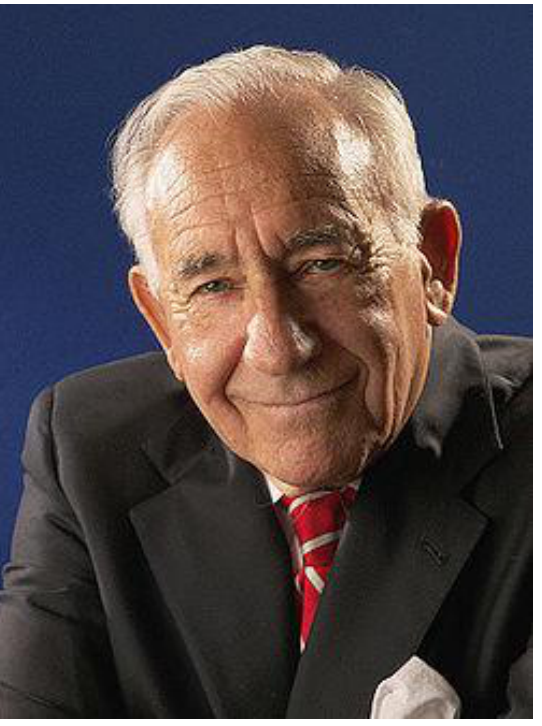
\includegraphics[width=59.22mm,height=199.58mm]{images/llm/page_038_img_01.png}%
\end{textblock*}

\newpage

% --- unit llm 39 ---
% === Halaman 39 (llm) ===

\section*{Ranah Steganografi}

Berdasarkan ranah operasinya, metode-metode steganografi dapat dibagi menjadi dua kelompok

\begin{itemize}
    \item \textbf{\textcolor{red}{Spatial (time) domain methods}}
    Memodifikasi langsung nilai $byte$ dari $cover-object$ (nilai $byte$ merepresentasikan intensitas/warna $pixel$ atau amplitudo)
    \par Contoh: Metode $LSB$
    
    \item \textbf{\textcolor{red}{Tranform domain methods}}
    Memodifikasi hasil transformasi sinyal dalam ranah transform (hasil transformasi dari ranah spasial ke ranah lain (misalnya ranah frekuensi).
    \par Contoh: Metode $Spread$ $Spectrum$
\end{itemize}

\newpage

% --- unit llm 40 ---
% === Halaman 40 (llm) ===

\begin{center}
\huge Metode LSB
\end{center}

\newpage

% --- unit llm 41 ---
% === Halaman 41 (llm) ===

\section*{Citra Digital}

\vspace{117.91mm}

\begin{itemize}
    \item Citra terdiri dari sejumlah \textit{pixel}. Citra $1200 \times 1500$ berarti memiliki $1200 \times 1500 \text{ pixel} = 1.800.000 \text{ pixel}$
\end{itemize}

\vspace{60mm}

\begin{itemize}
    \item Setiap \textit{pixel} panjangnya $n$-bit.
    \begin{itemize}
        \item Citra biner $\rightarrow 1 \text{ bit/pixel}$
        \item Citra \textit{grayscale} $\rightarrow 8 \text{ bit/pixel}$
        \item Citra \textit{true color} $\rightarrow 24 \text{ bit/pixel}$
    \end{itemize}
\end{itemize}

% deskripsi: Foto Taj Mahal sebagai contoh citra digital asli.
% bbox normalisasi: [0.1790, 0.2760, 0.4110, 0.6730]
\begin{textblock*}{48.72mm}(37.59mm,81.97mm)
\noindent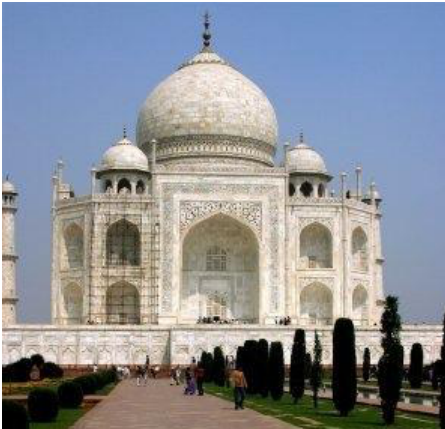
\includegraphics[width=48.72mm,height=117.91mm]{images/llm/page_041_img_01.png}%
\end{textblock*}

% deskripsi: Foto Taj Mahal dengan overlay grid yang mengilustrasikan konsep pixel pada citra digital.
% bbox normalisasi: [0.5110, 0.2670, 0.8310, 0.6980]
\begin{textblock*}{67.20mm}(107.31mm,79.30mm)
\noindent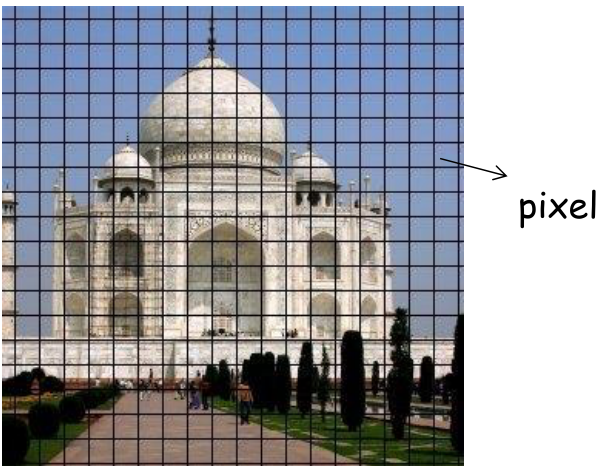
\includegraphics[width=67.20mm,height=128.01mm]{images/llm/page_041_img_02.png}%
\end{textblock*}

\newpage

% --- unit llm 42 ---
% === Halaman 42 (llm) ===

\section*{Citra Lenna}

\vspace{10mm}

\begin{center}
\begin{tabular}{ccc}
True color image & Grayscale image & Bimary image \\
(24-bit) & (8-bit) & (1-bit) \\
\end{tabular}
\end{center}

% deskripsi: Contoh citra Lenna dalam tiga format berbeda: warna asli (24-bit), skala abu-abu (8-bit), dan biner (1-bit).
% bbox normalisasi: [0.1200, 0.2500, 0.8600, 0.6200]
\begin{textblock*}{155.40mm}(25.20mm,74.25mm)
\noindent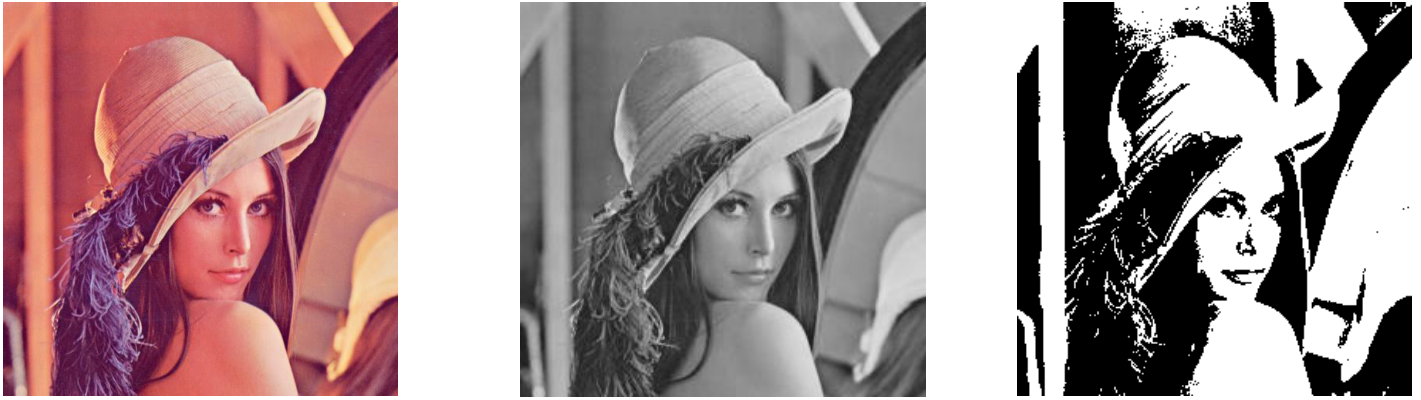
\includegraphics[width=155.40mm,height=109.89mm]{images/llm/page_042_img_01.png}%
\end{textblock*}

\newpage

% --- unit llm 43 ---
% === Halaman 43 (llm) ===

\vspace{190.08mm}

Pada citra 24-bit (\textit{real image}), 1 pixel = 24 bit, terdiri dari komponen RGB (Red-Green-Blue)

% deskripsi: Ilustrasi representasi warna sebuah pixel pada citra 24-bit menggunakan model RGB, menunjukkan sebuah pixel dari foto Taj Mahal yang dipetakan ke rangkaian bit biner yang dibagi menjadi tiga bagian: Red (merah), Green (hijau), dan Blue (biru).
% bbox normalisasi: [0.1410, 0.2860, 0.9060, 0.9260]
\begin{textblock*}{160.65mm}(29.61mm,84.94mm)
\noindent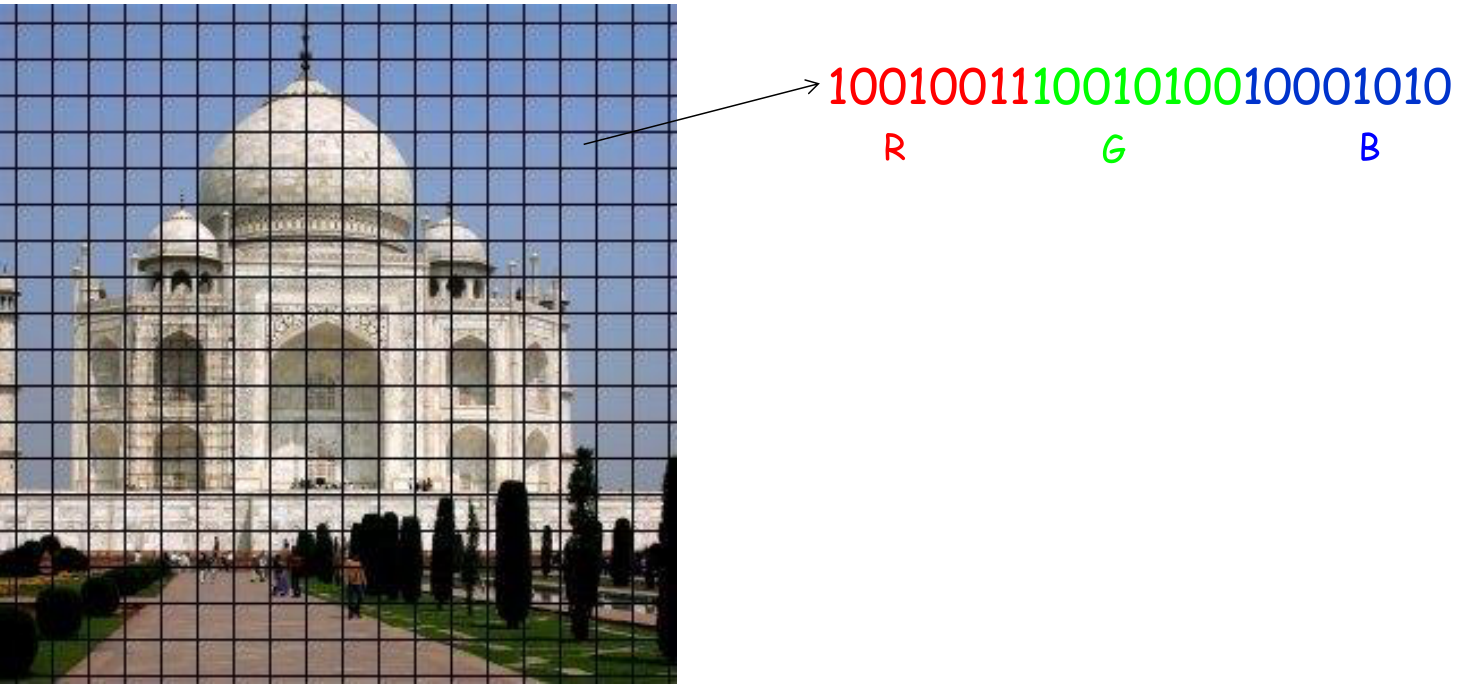
\includegraphics[width=160.65mm,height=190.08mm]{images/llm/page_043_img_01.png}%
\end{textblock*}

\newpage

% --- unit llm 44 ---
% === Halaman 44 (llm) ===

\section*{Metode LSB}

\begin{itemize}
    \item Di dalam setiap $byte$ bit-bitnya tersusun dari kiri ke kanan dalam urutan yang kurang berarti (\textit{least significant bits} atau LSB) hingga bit-bit yang berarti (\textit{most significant bits} atau MSB).
    \item Susunan bit pada setiap $byte$ adalah $b_7b_6b_5b_4b_3b_2b_1b_0$.
\end{itemize}

Contoh:

\vspace{30mm}

\begin{align*}
\text{Nilai dalam desimal} &= 1 \times 2^7 + 1 \times 2^6 + 0 \times 2^5 + 1 \times 2^4 + 0 \times 2^3 + 0 \times 2^2 + 0 \times 2^1 + 1 \times 2^0 = 209
\end{align*}

% deskripsi: Ilustrasi penentuan MSB (Most Significant Bit) dan LSB (Least Significant Bit) pada sebuah deret biner 11010001 menggunakan panah penunjuk.
% bbox normalisasi: [0.1900, 0.5800, 0.4080, 0.8200]
\begin{textblock*}{45.78mm}(39.90mm,172.26mm)
\noindent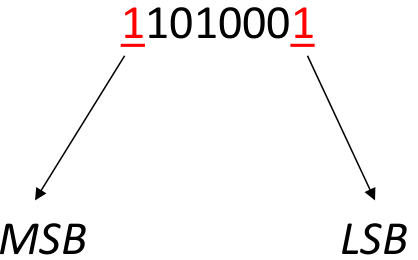
\includegraphics[width=45.78mm,height=71.28mm]{images/llm/page_044_img_01.png}%
\end{textblock*}

\newpage

% --- unit llm 45 ---
% === Halaman 45 (llm) ===

\begin{itemize}
    \item Mengubah nilai bit LSB tidak mengubah persepsi citra secara secara keseluruhan.
    \item Sebab, mengubah bit $LSB$ hanya mengubah nilai $byte$ satu lebih tinggi atau satu lebih rendah dari nilai sebelumnya.
\end{itemize}

\vspace{5mm}

Contoh: $1101000\text{1} \rightarrow 1101000\text{0}$
\[ (209) \quad (208) \]

\vspace{5mm}

Jika $1101000\text{1}$ misalnya menyatakan warna $\text{merah}$, maka $1101000\text{0}$ juga menyatakan warna $\text{merah}$ yang berubah sangat-sangat sedikit $\rightarrow$ tidakbisa dibedakan oleh mata manusia

\newpage

% --- unit llm 46 ---
% === Halaman 46 (llm) ===

Misalkan \underline{semua} bit LSB pada citra berwarna dibalikkan dari semula 0 menjadi 1; dari semula 1 menjadi 0

\vspace{10mm}

\begin{center}
\begin{tabular}{cc}
Sebelum & Sesudah
\end{tabular}
\end{center}

\begin{center}
\textcolor{red}{Adakah terlihat perbedaaannya?}
\end{center}

% deskripsi: Dua buah gambar perbandingan citra berwarna kapal layar, satu sebelum manipulasi bit LSB dan satu setelah manipulasi bit LSB, yang terlihat hampir identik.
% bbox normalisasi: [0.1500, 0.2400, 0.8500, 0.8200]
\begin{textblock*}{147.00mm}(31.50mm,71.28mm)
\noindent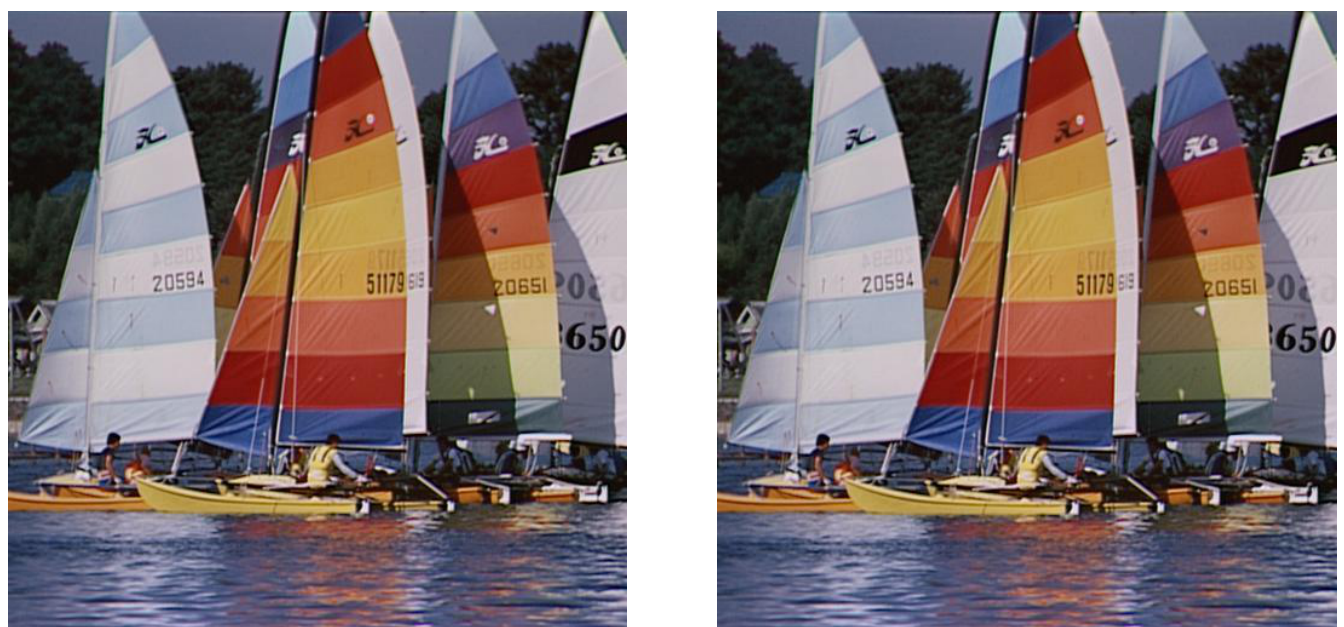
\includegraphics[width=147.00mm,height=172.26mm]{images/llm/page_046_img_01.png}%
\end{textblock*}

\newpage

% --- unit llm 47 ---
% === Halaman 47 (llm) ===

\vspace{172.26mm}

Misalkan $\underline{\text{semua}}$ bit LSB pada citra $grayscale$ dibalikkan\\Dari semula 0 menjadi 1; dari semula 1 menjadi 0
\vspace{20mm}
\begin{center}
Sebelum \hspace{5cm} Sesudah
\end{center}
\begin{center}
\textcolor{red}{Adakah terlihat perbedaaanya?}
\end{center}

% deskripsi: Perbandingan dua citra grayscale sebuah gedung sebelum dan sesudah manipulasi bit LSB (Least Significant Bit), di mana citra kiri berlabel 'Sebelum' dan citra kanan berlabel 'Sesudah'.
% bbox normalisasi: [0.1500, 0.2300, 0.8500, 0.8100]
\begin{textblock*}{147.00mm}(31.50mm,68.31mm)
\noindent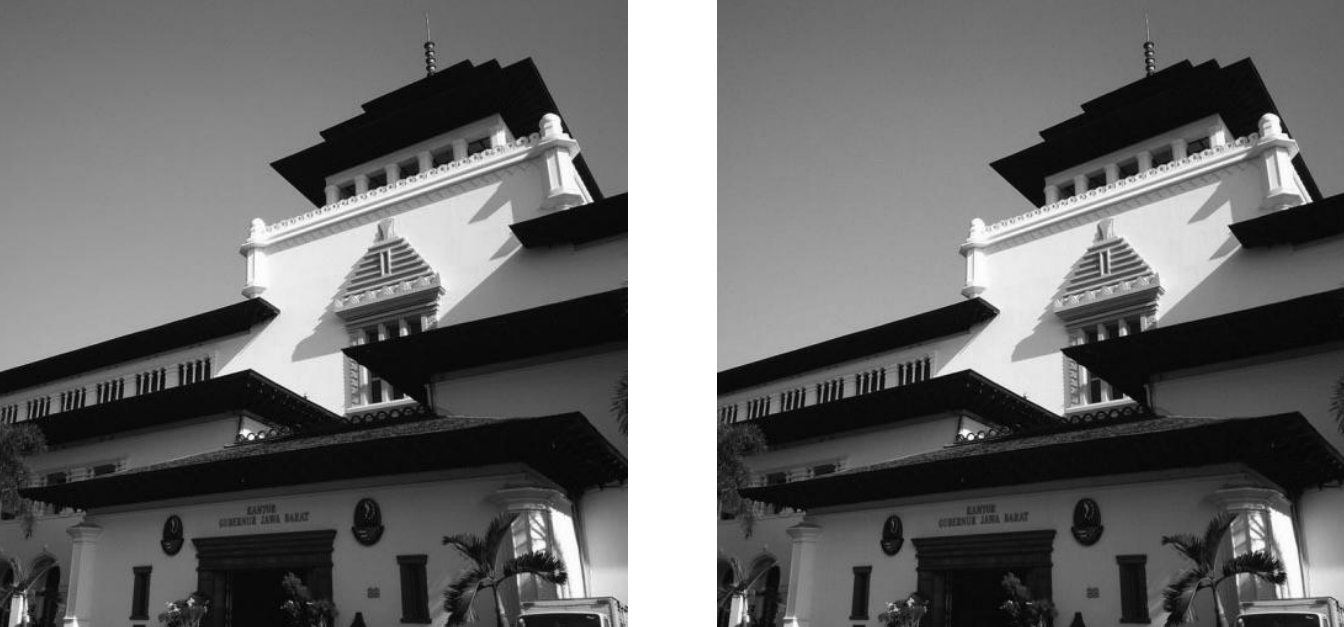
\includegraphics[width=147.00mm,height=172.26mm]{images/llm/page_047_img_01.png}%
\end{textblock*}

\newpage

% --- unit llm 48 ---
% === Halaman 48 (llm) ===

\section*{Contoh 1:}

\begin{itemize}
    \item Tinjau 1 buah $pixel$ dari citra 24-bit ($3 \times 8$ bit):
    
    \begin{center}
        \color{red}10000010 \quad \color{red}01111011 \quad \color{red}01110101 \\
        (130) \quad (123) \quad (117)
    \end{center}

    \item Bit bit-bit $embedded\ message$: \color{blue}101
    
    \item $Embed$: \color{red}0011001\color{blue}1 \quad \color{red}1010001\color{blue}0 \quad \color{red}1110001\color{blue}1
\end{itemize}

\vspace{30mm}

Original: misalkan $pixel\ [130, 123, 117]$ berwarna ``ungu'' \\
Stego-image: $pixel\ [131, 122, 117]$ tetap ``ungu'' tapi berubah sangat sedikit. Mata manusia tidak dapat membedakan perubahan warna yang sangat kecil.

% deskripsi: Ilustrasi proses steganografi LSB pada pixel gambar, menunjukkan perubahan bit terakhir (LSB) dari warna original ke stego-image berdasarkan pesan 101.
% bbox normalisasi: [0.1430, 0.5660, 0.7680, 0.7880]
\begin{textblock*}{131.25mm}(30.03mm,168.10mm)
\noindent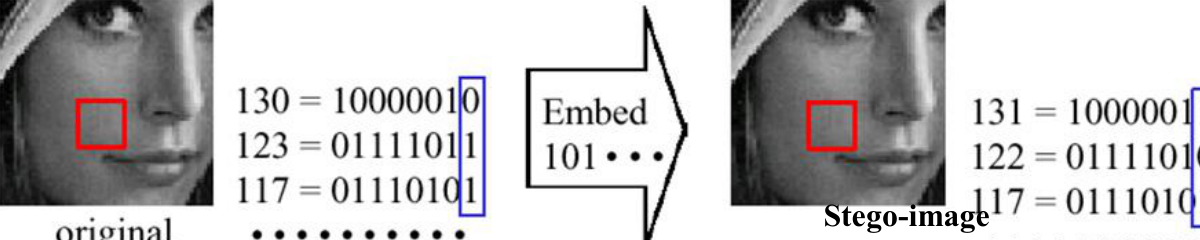
\includegraphics[width=131.25mm,height=65.93mm]{images/llm/page_048_img_01.png}%
\end{textblock*}

\newpage

% --- unit llm 49 ---
% === Halaman 49 (llm) ===

Pergeseran warna sebesar 1 dari 256 warna tidak dapat dilihat oleh manusia

\vspace{20mm}

Sumber: TA Yulie Anneria Sinaga 13504085

% deskripsi: Gambar contoh steganografi yang menunjukkan foto paprika berwarna-warni dengan teks tersembunyi 'PESAN RAHASIA' dan deretan angka biner di sisi kanan.
% bbox normalisasi: [0.3300, 0.3200, 0.6670, 0.8870]
\begin{textblock*}{70.77mm}(69.30mm,95.04mm)
\noindent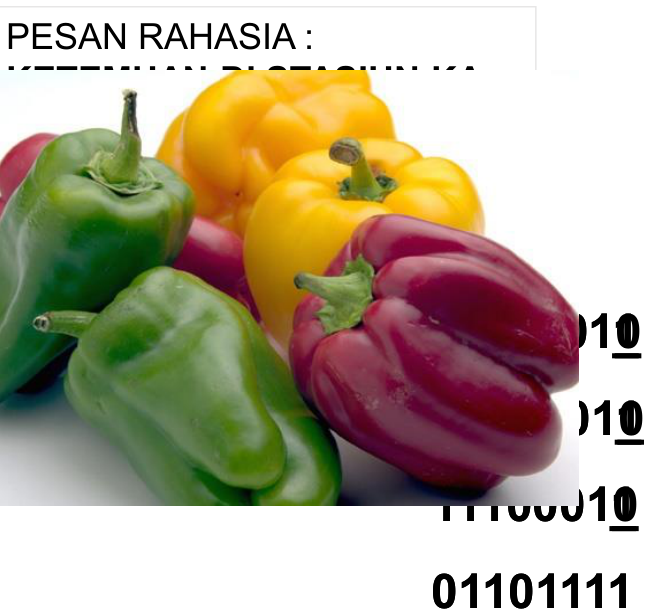
\includegraphics[width=70.77mm,height=168.40mm]{images/llm/page_049_img_01.png}%
\end{textblock*}

\newpage

% --- unit llm 50 ---
% === Halaman 50 (llm) ===

Contoh 2:

\begin{itemize}
    \item Jika pesan = 10 bit, maka jumlah \textit{byte} yang digunakan = 10 \textit{byte}
    \item Contoh susunan \textit{byte} yang lebih panjang:
    \begin{center}
    \texttt{00110011 10100010 11100010 10101011 00100110}\
    \texttt{10010110 11001001 11111001 10001000 10100011}
    \end{center}
    \item Pesan: 1110010111
    \item Hasil penyisipan pada bit \textit{LSB}:
    \begin{center}
    \texttt{00110011 10100011 11100011 10101010 00100110}\
    \texttt{10010111 11001000 11111001 10001001 10100011}
    \end{center}
\end{itemize}

\newpage

% --- unit llm 51 ---
% === Halaman 51 (llm) ===

\section*{Ekstraksi Pesan dari $Stego\text{-}image$}

\begin{itemize}
    \item Bit-bit pesan yang disembunyikan di dalam citra harus dapat diekstraksi kembali.
    \item Caranya adalah dengan membaca $byte\text{-}byte$ di dalam citra, mengambil LSB-nya, dan merangkainya kembali menjadi bit-bit pesan.
    \item Contoh: Misalkan $stego\text{-}object$ adalah sbb
\end{itemize}

\vspace{5mm}

Ekstrak bit-bit LSB: $\mathbf{1110010111}$

% deskripsi: Contoh representasi biner dari stego-object dengan bit LSB yang diwarnai biru untuk menunjukkan proses ekstraksi.
% bbox normalisasi: [0.1060, 0.6020, 0.6820, 0.7150]
\begin{textblock*}{120.96mm}(22.26mm,178.79mm)
\noindent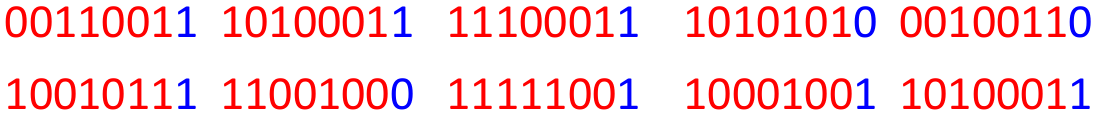
\includegraphics[width=120.96mm,height=33.56mm]{images/llm/page_051_img_01.png}%
\end{textblock*}

\newpage

% --- unit llm 52 ---
% === Halaman 52 (llm) ===

\section*{Menghitung Ukuran Pesan yang dapat Disembunyikan}

\begin{itemize}
    \item Ukuran pesan yang akan disembunyikan bergantung pada ukuran \textit{cover-object}.
    \item Misalkan pada citra \textit{grayscale} (1 byte/pixel) $256 \times 256$ \textit{pixel} :
    \begin{itemize}
        \item jumlah \textit{pixel} = jumlah byte = $256 \times 256 = 65536$
        \item setiap byte dapat menyembunyikan 1 bit pesan di LSB-nya
        \item jadi ukuran maksimal pesan = $65536$ bit = $8192$ \textit{byte} = 8 KB
    \end{itemize}
    \item Pada citra berwarna 24-bit berukuran $256 \times 256$ \textit{pixel}:
    \begin{itemize}
        \item jumlah \textit{pixel} $256 \times 256 = 65536$
        \item setiap pixel = 3 byte, berarti ada $65536 \times 3 = 196608$ \textit{byte}.
        \item setiap \textit{byte} dapat menyembunyikan 1 bit pesan
        \item jadi ukuran maksimal pesan = $196608$ bit = $24576$ byte = 24KB
    \end{itemize}
\end{itemize}

\newpage

% --- unit llm 53 ---
% === Halaman 53 (llm) ===

\section*{Beberapa Varian Metode LSB}

\vspace{127.12mm}

\subsection*{1. Sequential}
\begin{itemize}
    \item Bit-bit pesan disembunyikan secara sekuensial pada \textit{pixel-pixel} citra.
    \item Misalkan ukuran pesan = 15 bit, maka urutan \textit{pixel-pixel} yang digunakan untuk penyembunyian bit adalah:
\end{itemize}
\vspace{10mm}

% deskripsi: Tabel representasi grid pixel yang menunjukkan urutan penempatan bit pesan dari 1 sampai 15 secara sekuensial.
% bbox normalisasi: [0.3100, 0.4580, 0.6010, 0.8860]
\begin{textblock*}{61.11mm}(65.10mm,136.03mm)
\noindent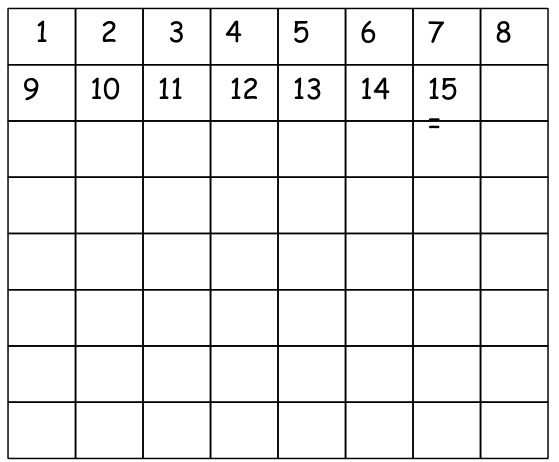
\includegraphics[width=61.11mm,height=127.12mm]{images/llm/page_053_img_01.png}%
\end{textblock*}

\newpage

% --- unit llm 54 ---
% === Halaman 54 (llm) ===

\section*{Ekstraksi pesan dari Stego-image}

\begin{itemize}
    \item Pada proses ekstraksi pesan, \textit{pixel-pixel} dibaca secara sekuensial mulai dari \textit{pixel} pertama sampai \textit{pixel} yang menyimpan bit pesan terakhir
    \item Ambil setiap \textit{byte} dari \textit{pixel}, ekstraksi bit LSB-nya.
    \item Rangkailah bit-bit LSB menjadi bit-bit pesan semula.
\end{itemize}

\newpage

% --- unit llm 55 ---
% === Halaman 55 (llm) ===

\section*{2. Acak}

\begin{itemize}
    \item Untuk membuat penyembunyian pesan lebih aman, bit-bit pesan tidak disimpan pada pixel-pixel yang berurutan, namun dipilih secara acak.
    \item Pembangkit bilangan acak-semu (PRNG: \textit{pseudo-random number generator}) digunakan untuk membangkitkan bilangan acak.
    \item Umpan (\textit{seed}) untuk pembangkit bilangan acak berlaku sebagai kunci (\textit{stego-key}).
\end{itemize}

\newpage

% --- unit llm 56 ---
% === Halaman 56 (llm) ===

\begin{itemize}
    \item Misalnya jika terdapat 64 $byte$ dan 15 bit pesan yang akan disembunyikan. $Pixel-pixel$ dipilih secara acak, seperti pada gambar berikut.
\end{itemize}

\vspace{10mm}

% deskripsi: Grid 8x8 yang merepresentasikan pixel-pixel, dengan beberapa sel berisi angka yang menunjukkan urutan pemilihan pixel secara acak untuk menyembunyikan bit pesan.
% bbox normalisasi: [0.3130, 0.4080, 0.6030, 0.8310]
\begin{textblock*}{60.90mm}(65.73mm,121.18mm)
\noindent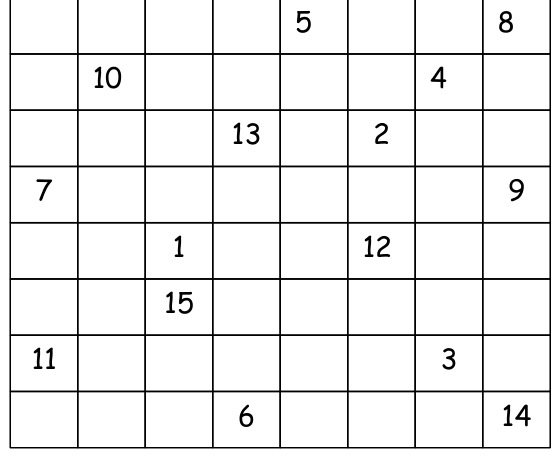
\includegraphics[width=60.90mm,height=125.63mm]{images/llm/page_056_img_01.png}%
\end{textblock*}

\newpage

% --- unit llm 57 ---
% === Halaman 57 (llm) ===

\section*{Ekstraksi pesan dari \textit{Stego-image}}

\begin{itemize}
    \item Posisi \textit{pixel} yang menyimpan bit pesan dapat diketahui dari bilangan acak yang dibangkitkan oleh \textit{PRNG}.
    \item Jika kunci yang digunakan pada waktu ekstraksi sama dengan kunci pada waktu penyisipan, maka bilangan acak yang dibangkitkan juga sama.
    \item Dengan demikian, bit-bit pesan yang bertaburan di dalam citra dapat dikumpulkan kembali.
\end{itemize}

\newpage

% --- unit llm 58 ---
% === Halaman 58 (llm) ===

\section*{3. $m$-bit LSB}

\begin{itemize}
    \item Untuk meningkatkan ukuran pesan yang disembunyikan, maka digunakan lebih dari 1 bit LSB untuk setiap \textit{byte}.
    \item Susunan bit pada setiap \textit{byte} adalah $b_7b_6b_5b_4b_3b_2b_1b_0$. Jika diambil 2-bit LSB, maka bit yang digunakan adalah bit $b_1$ dan bit $b_0$.
    
    Contoh: $110100\underline{10} \rightarrow 2$ bit LSB terakhir dipakai untuk menyembunyikan pesan.
    
    \item \textit{Trade-off}: Semakin banyak bit LSB yang digunakan, semakin besar ukuran pesan yang dapat disembunyikan, tetapi semakin turun kualitas \textit{stego-image}.
    \item Pesan dapat disembunyikan secara sekuensial atau secara acak pada \textit{pixel-pixel} di dalam citra.
\end{itemize}

\newpage

% --- unit llm 59 ---
% === Halaman 59 (llm) ===

\section*{4. Enkripsi}

\begin{itemize}
    \item Pesan dapat dienkripsi terlebih dahulu sebelum disembunyikan ke dalam citra.
    \item Teknik enkripsi yang sederhana misalnya dengan meng-XOR-kan bit-bit pesan dengan bit-bit kunci. Jumlah bit-bit kunci sama dengan jumlah bit pesan.
    \item Bit-bit kunci dibangkitkan secara acak.
    \item Kunci untuk pembangkitan bit-bit kunci menjadi \textit{stego-key}.
    \item Jika dipakai teknik acak dalam memilih \textit{pixel-pixel}, maka ada dua \textit{stego-key}: satu untuk pembangkitan bit-bit kunci, satu lagi untuk pembangkitan posisi \textit{pixel} yang dipilih untuk menyembunyikan pesan.
\end{itemize}

\newpage

% --- unit llm 60 ---
% === Halaman 60 (llm) ===

\section*{Demo Steganografi Online}

\begin{itemize}
    \item \url{https://www.edchart.com/free-online-converters/image-steganography.php}
    \item \url{https://planetcalc.com/9345/}
    \item \url{https://georgeom.net/StegOnline/upload}
    \item \url{https://incoherency.co.uk/image-steganography/}
    \item \url{https://steghide.sourceforge.net/} (aplikasi freeware)
\end{itemize}

\newpage

% --- unit llm 61 ---
% === Halaman 61 (llm) ===

\section*{Free Online Image steganography Encoder tool}

\vspace{163.35mm}

The image steganography tool allows you to embed hidden data inside a carrier file, such as an image. You could extract data from Free Online Image Steganographic DecoderTool .

% deskripsi: Screenshot antarmuka web tool Encoder Steganografi Gambar yang mencakup opsi untuk memilih gambar, memasukkan teks yang ingin disembunyikan, dan kolom kata sandi.
% bbox normalisasi: [0.2300, 0.3300, 0.8100, 0.8800]
\begin{textblock*}{121.80mm}(48.30mm,98.01mm)
\noindent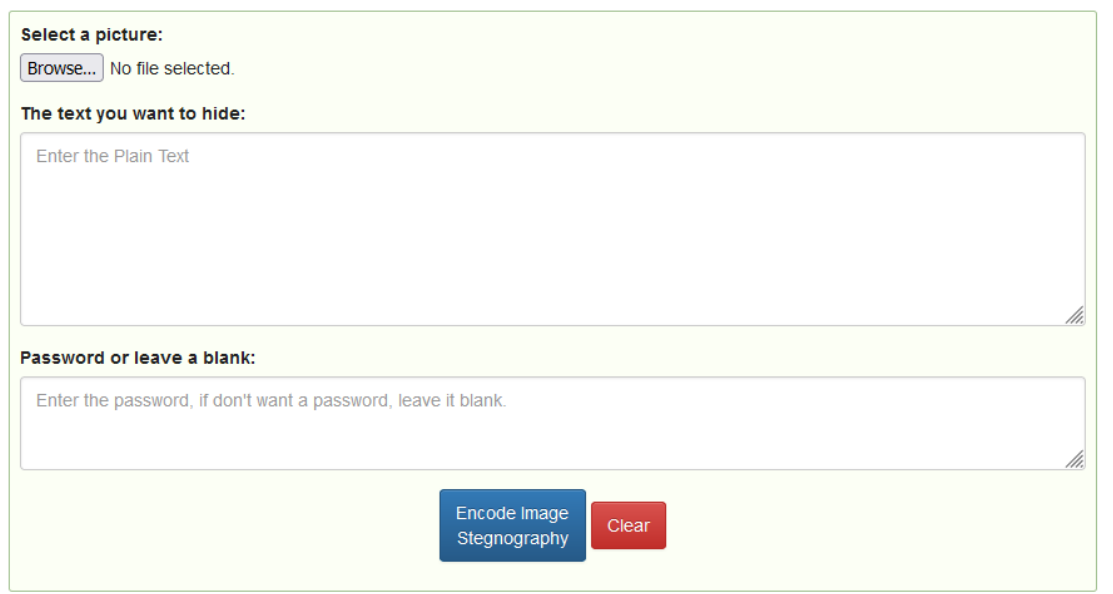
\includegraphics[width=121.80mm,height=163.35mm]{images/llm/page_061_img_01.png}%
\end{textblock*}

\newpage

% --- unit llm 62 ---
% === Halaman 62 (llm) ===

PLANETCALC Online calculators

\vspace{10mm}

Hide information inside picture

\vspace{187.11mm}

Message

We are discovered. Flee at once

\vspace{5mm}

Source image

\begin{tabular}{|l|l|}
\hline
File & Size \\ \hline
sushi-text.png & 2Kb \hline
\end{tabular}

\vspace{5mm}

CALCULATE

% deskripsi: Screenshot antarmuka kalkulator online untuk menyembunyikan informasi di dalam gambar (steganografi) yang menampilkan kotak pesan, area unggah file gambar, dan tombol hitung.
% bbox normalisasi: [0.0600, 0.2900, 0.7100, 0.9200]
\begin{textblock*}{136.50mm}(12.60mm,86.13mm)
\noindent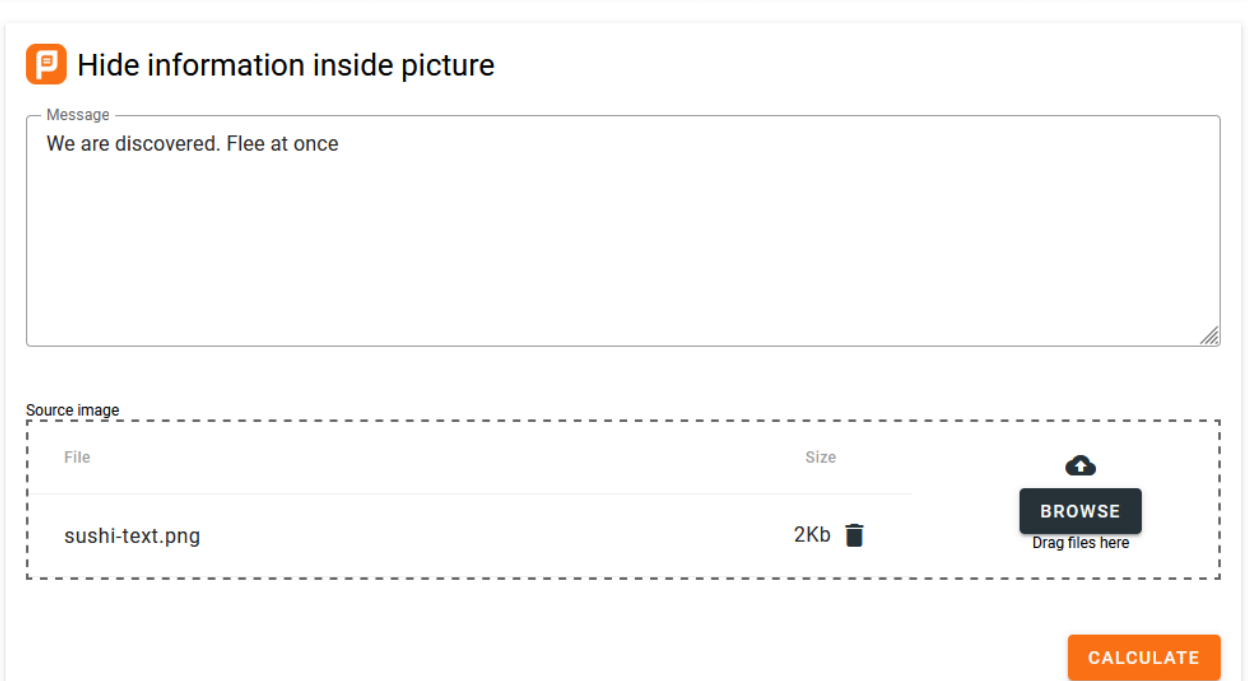
\includegraphics[width=136.50mm,height=187.11mm]{images/llm/page_062_img_01.png}%
\end{textblock*}

\newpage

% --- unit llm 63 ---
% === Halaman 63 (llm) ===

\ hyperlinks{https://georgeom.net/StegOnline/upload}

\vspace{10mm}

StegOnline

Upload $\quad$ CTF Checklist $\quad$ About

UPLOAD IMAGE

Drag and drop your image here

% deskripsi: Screenshot halaman web StegOnline yang menampilkan antarmuka pengunggahan gambar untuk steganografi.
% bbox normalisasi: [0.0600, 0.1200, 0.9400, 0.6500]
\begin{textblock*}{184.80mm}(12.60mm,35.64mm)
\noindent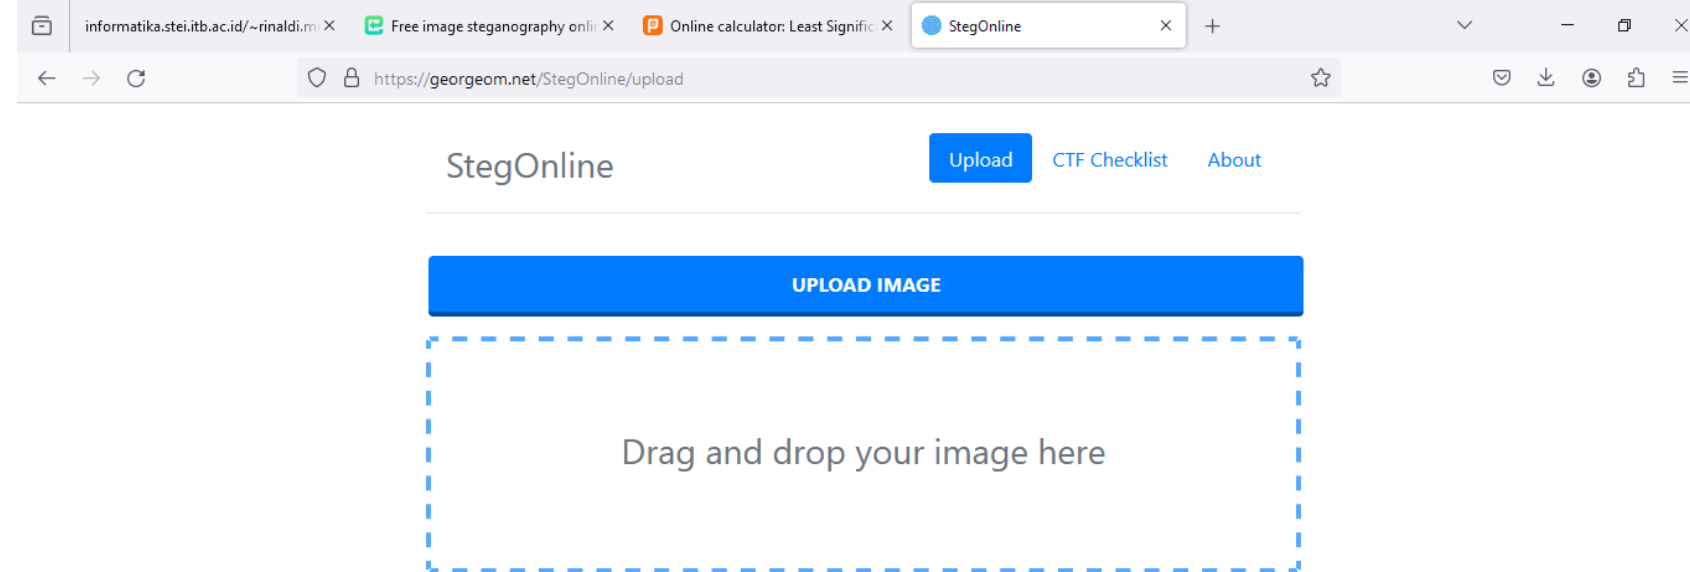
\includegraphics[width=184.80mm,height=157.41mm]{images/llm/page_063_img_01.png}%
\end{textblock*}

\newpage

% --- unit llm 64 ---
% === Halaman 64 (llm) ===

\section*{How to Hack a Computer Using Just An Image}
\noindent Monday, June 01, 2015 $\bullet$ Swati Khandelwal

\vspace{20mm}

Next time when someone sends you a photo of a cute cat or a hot chick then be careful before you CLICK on the image to view --- it might hack your machine.

Yes, the normal looking images could hack your computers --- thanks to a technique discovered by security researcher \textit{Saumil Shah} from India.

\vspace{59.40mm}

Dubbed \quot{Stegospolit\quot, the technique lets hackers hide malicious code inside the pixels of an image, hiding a malware exploit in plain sight to infect target victims.

\textbf{Just look at the image and you are HACKED!}

\url{http://thehackernews.com/2015/06/Stegospolit-malware.html}

% deskripsi: Screenshot artikel yang menunjukkan gambar kucing dengan teks 'THIS PICTURE CAN HACK YOUR COMPUTER' dan latar belakang kode biner.
% bbox normalisasi: [0.1700, 0.1300, 0.6600, 0.5900]
\begin{textblock*}{102.90mm}(35.70mm,38.61mm)
\noindent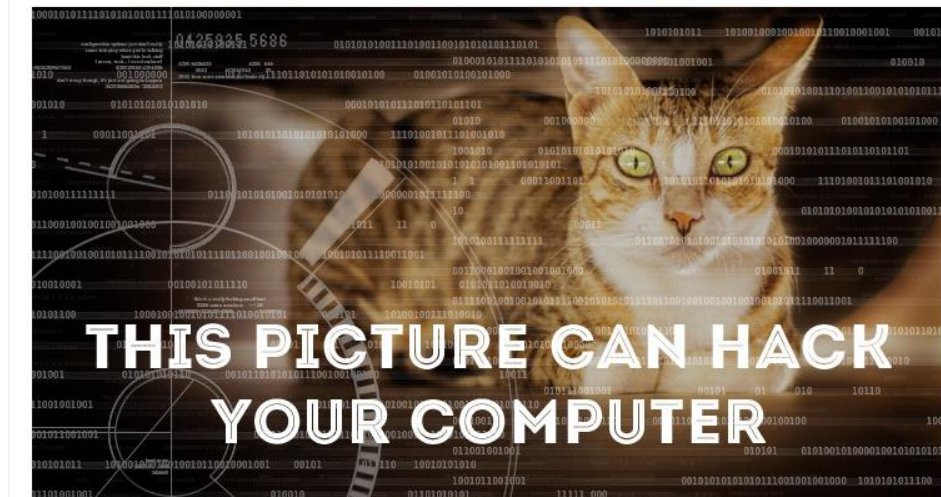
\includegraphics[width=102.90mm,height=136.62mm]{images/llm/page_064_img_01.png}%
\end{textblock*}

% deskripsi: Screenshot layar terminal komputer berwarna hitam dengan teks hijau bertuliskan 'ACCESS GRANTED'.
% bbox normalisasi: [0.7100, 0.6400, 0.8800, 0.8400]
\begin{textblock*}{35.70mm}(149.10mm,190.08mm)
\noindent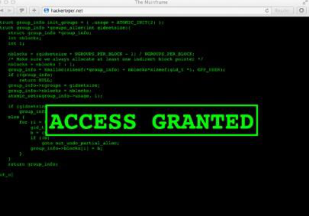
\includegraphics[width=35.70mm,height=59.40mm]{images/llm/page_064_img_02.png}%
\end{textblock*}

\newpage

% --- unit llm 65 ---
% === Halaman 65 (llm) ===

\section*{Program Steganografi dengan MATLAB}

\begin{itemize}
    \item Kode program Matlab berikut ini menyisipkan pesan dengan metode LSB.
\end{itemize}

\textbf{A. Program penyisipan pesan}
\begin{itemize}
    \item Input:
    \begin{enumerate}
        \item Citra berwarna (RGB)
        \item Pesan (diketik langsung dari keyboard)
    \end{enumerate}
    \item Output: citra stego (stego image)
\end{itemize}

\textbf{B. Program ekstraksi pesan}
\begin{itemize}
    \item Input: Citra stego
    \item Output: pesan
\end{itemize}

\newpage

% --- unit llm 66 ---
% === Halaman 66 (llm) ===

\section*{A. Program penyisipan pesan}

\begin{verbatim}
% Nama file: LSB_sisip.m
% Penyisipan pesan di dalam citra dengan metode modifikasi LSB. Panjang
% pesan (L) disimpan di dalam citra stegano.
% Asumsi: jumlah bit untuk merepresentasikan panjang pesan maksimal 30 bit.
% Input: 1. Citra berwarna (RGB)
%        2. Teks dari keyboard
% Output: citra stego (harus disimpan dalam format BMP)
% Diprogram oleh Rinaldi Munir, @Informatika STEI-ITB

clear all;
% Baca citra cover dan tampilkan
namaFile = input('Ketikkan nama file citra cover: ', 's');
coverImage = imread(namaFile);
imshow(namaFile); title ('Citra cover ');

tinggi = size(coverImage, 1);
lebar = size(coverImage, 2);
total_byte = tinggi * lebar * 3;
total_bit_embed = total_byte;

% Baca pesan
pesan = input('Ketikkan pesan: ', 's');
\end{verbatim}

\newpage

% --- unit llm 67 ---
% === Halaman 67 (llm) ===

\begin{verbatim}
% Baca pesan
pesan = input('Ketikkan pesan: ', 's');

\vspace{213.84mm}

% Hitung panjang pesan
L = length(pesan);

%Konversi panjang pesan ke dalam biner
nL = dec2bin(L, 30);

%Konversi pesan ke dalam vektor biner
for i = 1 : L
  biner((i-1)*8 + 1 : i*8) = dec2bin(pesan(i), 8);
end

% Gabungkan bit-bit panjang pesan dengan bit-bit pesan
biner = [nL, biner];
m = length(biner);     % Ubah vektor biner ke numerik

if m > total\_bit\_embed
  disp('Ukuran citra tidak mencukup untuk penyembunyian pesan');
end
\end{verbatim}

% deskripsi: Screenshot potongan kode program MATLAB untuk proses konversi pesan teks menjadi biner dalam konteks steganografi.
% bbox normalisasi: [0.0380, 0.1300, 0.6050, 0.8500]
\begin{textblock*}{119.07mm}(7.98mm,38.61mm)
\noindent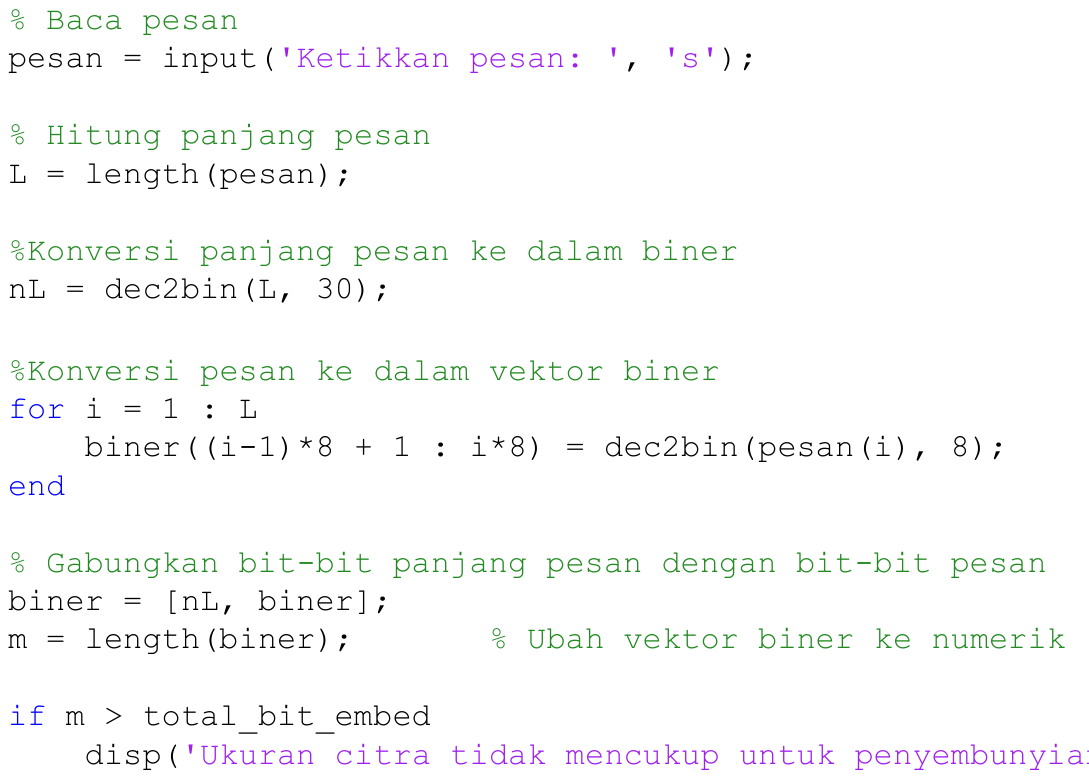
\includegraphics[width=119.07mm,height=213.84mm]{images/llm/page_067_img_01.png}%
\end{textblock*}

\newpage

% --- unit llm 68 ---
% === Halaman 68 (llm) ===

\vspace{270.27mm}

else
\begin{verbatim}
biner = biner(:);             % Transpose vektor biner
biner = str2num(biner);      % Ubah bit biner ke numerik

% Lakukan penyisipan bit-bit pesan ke dalam pixel-pixel
disp('Penyisipan pesan....');
idx = 1; % Mulai dari bit pertama pesan
for row = 1 : size(coverImage,1)
    for col = 1 : size(coverImage,2)
        for i = 1 : 3
            if idx <= m
                coverImage(row, col, i) = bitset(coverImage(row, col, i), 1, biner(idx));
                idx = idx + 1;
            end
        end
    end
end
stegoImage = coverImage;
% Simpan citra stego
namaFile = input('Ketikkan nama file citra stego (bmp): ', 's');
imwrite(stegoImage, namaFile);
% Tampilkan citra stego
figure; imshow(stegoImage); title ('Citra steo');
disp('Selesai');
end
\end{verbatim}

% deskripsi: Screenshot potongan kode pemrograman MATLAB untuk proses penyisipan bit pesan ke dalam citra (steganografi)
% bbox normalisasi: [0.0500, 0.0300, 0.9700, 0.9400]
\begin{textblock*}{193.20mm}(10.50mm,8.91mm)
\noindent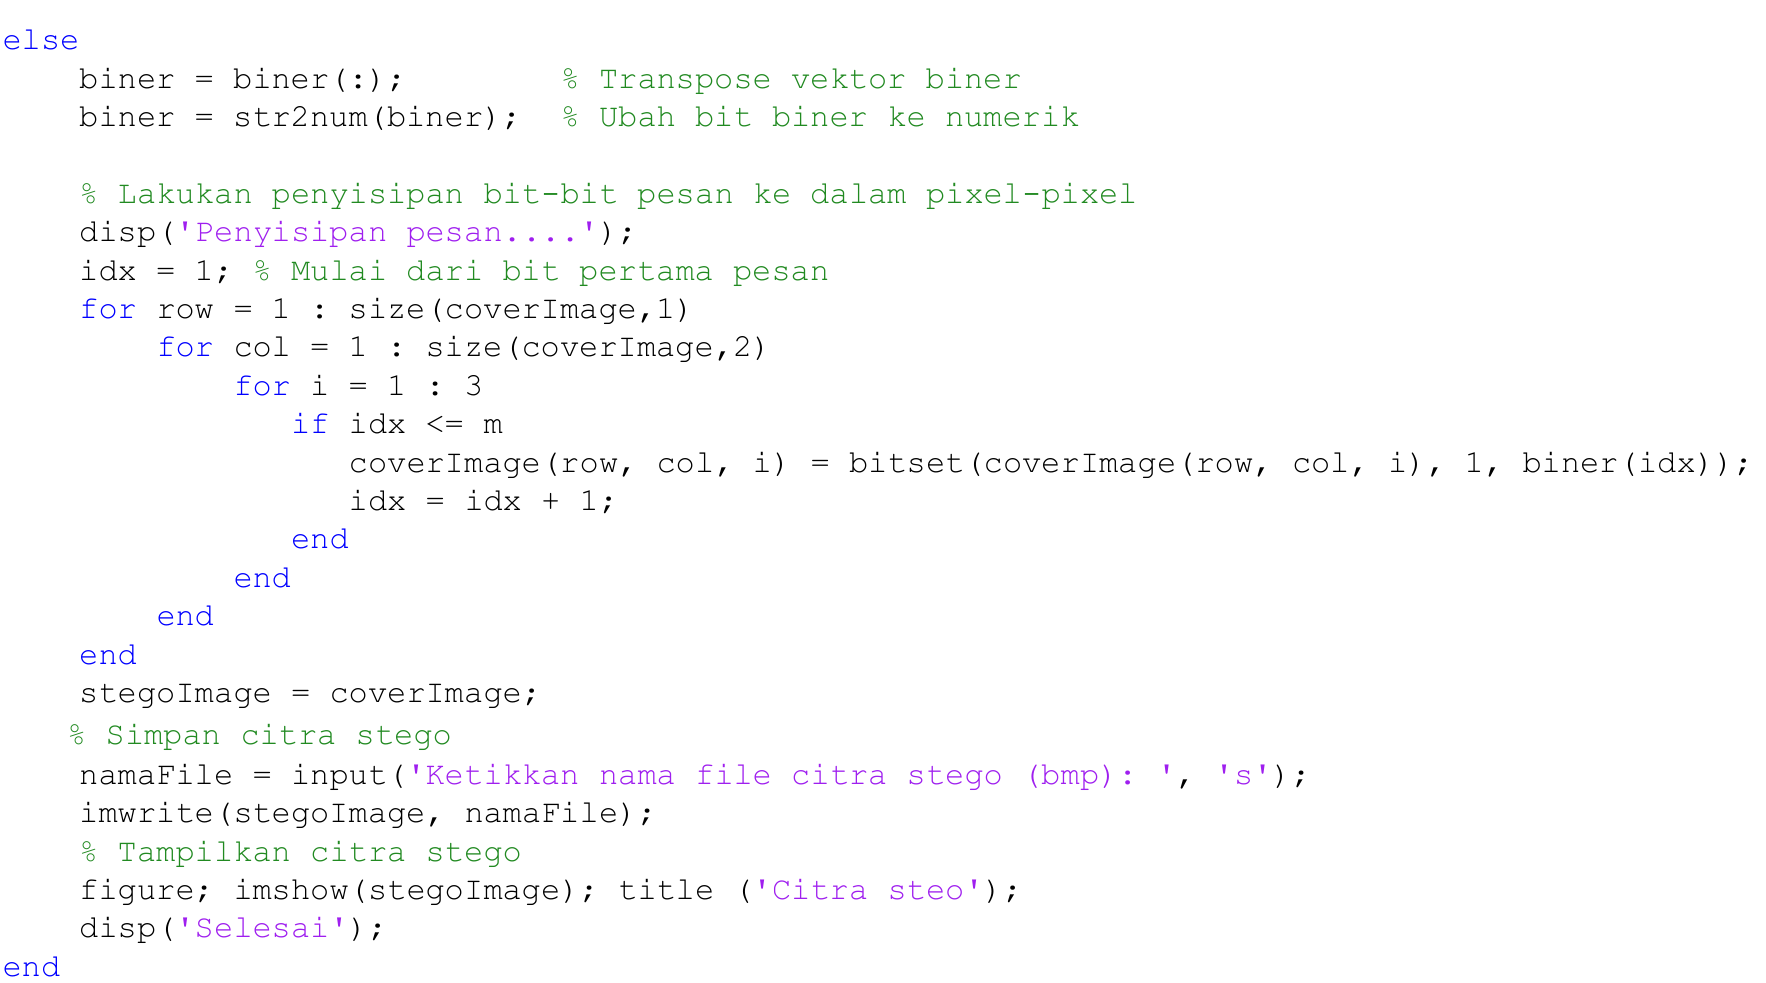
\includegraphics[width=193.20mm,height=270.27mm]{images/llm/page_068_img_01.png}%
\end{textblock*}

\newpage

% --- unit llm 69 ---
% === Halaman 69 (llm) ===

\textbf{Running program:}

\vspace{170.77mm}

>> LSB\_sisip\nKetikkan nama file citra cover: peppers.bmp\nKetikkan pesan: Mari kita jaga negara kesatuan Republik Indonesia tercinta. Oke?\nPenyisipan pesan....\nKetikkan nama file citra stego (bmp): output.bmp\nSelesai\n>>

% deskripsi: Screenshot jendela program yang menampilkan 'Citra cover' berisi gambar paprika warna-warni.
% bbox normalisasi: [0.1270, 0.4080, 0.4360, 0.9830]
\begin{textblock*}{64.89mm}(26.67mm,121.18mm)
\noindent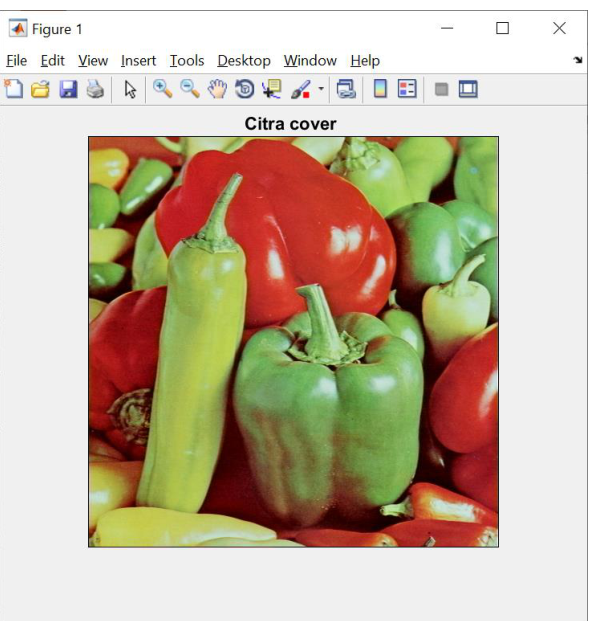
\includegraphics[width=64.89mm,height=170.77mm]{images/llm/page_069_img_01.png}%
\end{textblock*}

% deskripsi: Screenshot jendela program yang menampilkan 'Citra stego' berisi gambar paprika yang secara visual terlihat identik dengan citra cover.
% bbox normalisasi: [0.5030, 0.4080, 0.8320, 0.9830]
\begin{textblock*}{69.09mm}(105.63mm,121.18mm)
\noindent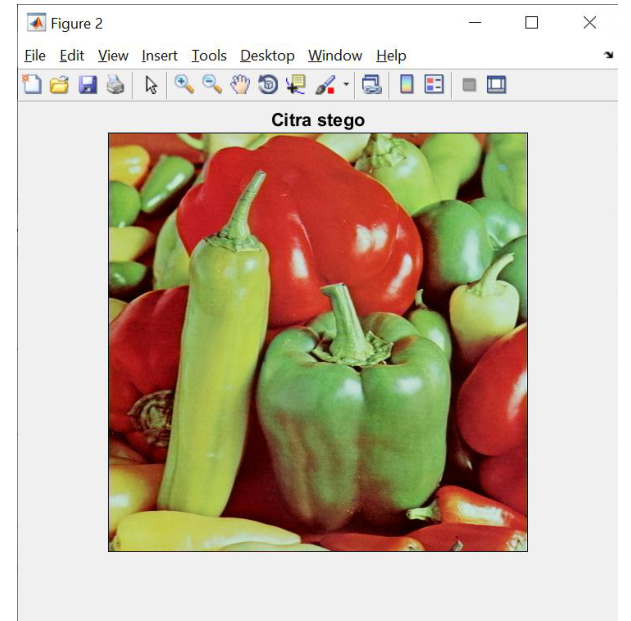
\includegraphics[width=69.09mm,height=170.77mm]{images/llm/page_069_img_02.png}%
\end{textblock*}

\newpage

% --- unit llm 70 ---
% === Halaman 70 (llm) ===

\section*{B. Program ekstraksi pesan}

\vspace{252.45mm}

\begin{verbatim}
% Nama file: LSB_estrak.m
% Ekstraksi pesan dari citra stegano dengan metode modifikasi LSB. Panjang
% pesan (L) telah disimpan di dalam citra stegano.
% Asumsi: jumlah bit untuk merepresentasikan panjang pesan maksimal 30 bit.
% Input: Citra stegano (berwarna)
% Output: pesan (teks)
% Diprogram oleh Rinaldi Munir, @Informatika STEI-ITB

clear all;

% Baca citra stegano
namaFile = input('Ketikkan nama file citra stego: ', 's');
stegoImage = imread(namaFile);
imshow(namaFile); title ('Citra stego ');

% Ekstraksi bit-bit panjang pesan terlebih dahulu
% Diperlukan 30 byte = 10 pixel x 3 byte pada baris pertama citra stegano
idx = 1;
for col = 1:10
    for i = 1:3
        nL(idx) = bitget(stegoImage(1,col, i), 1);
        idx = idx + 1;
    end
end
\end{verbatim}

% deskripsi: Screenshot potongan kode MATLAB untuk program ekstraksi pesan menggunakan metode LSB.
% bbox normalisasi: [0.0500, 0.1100, 0.8000, 0.9600]
\begin{textblock*}{157.50mm}(10.50mm,32.67mm)
\noindent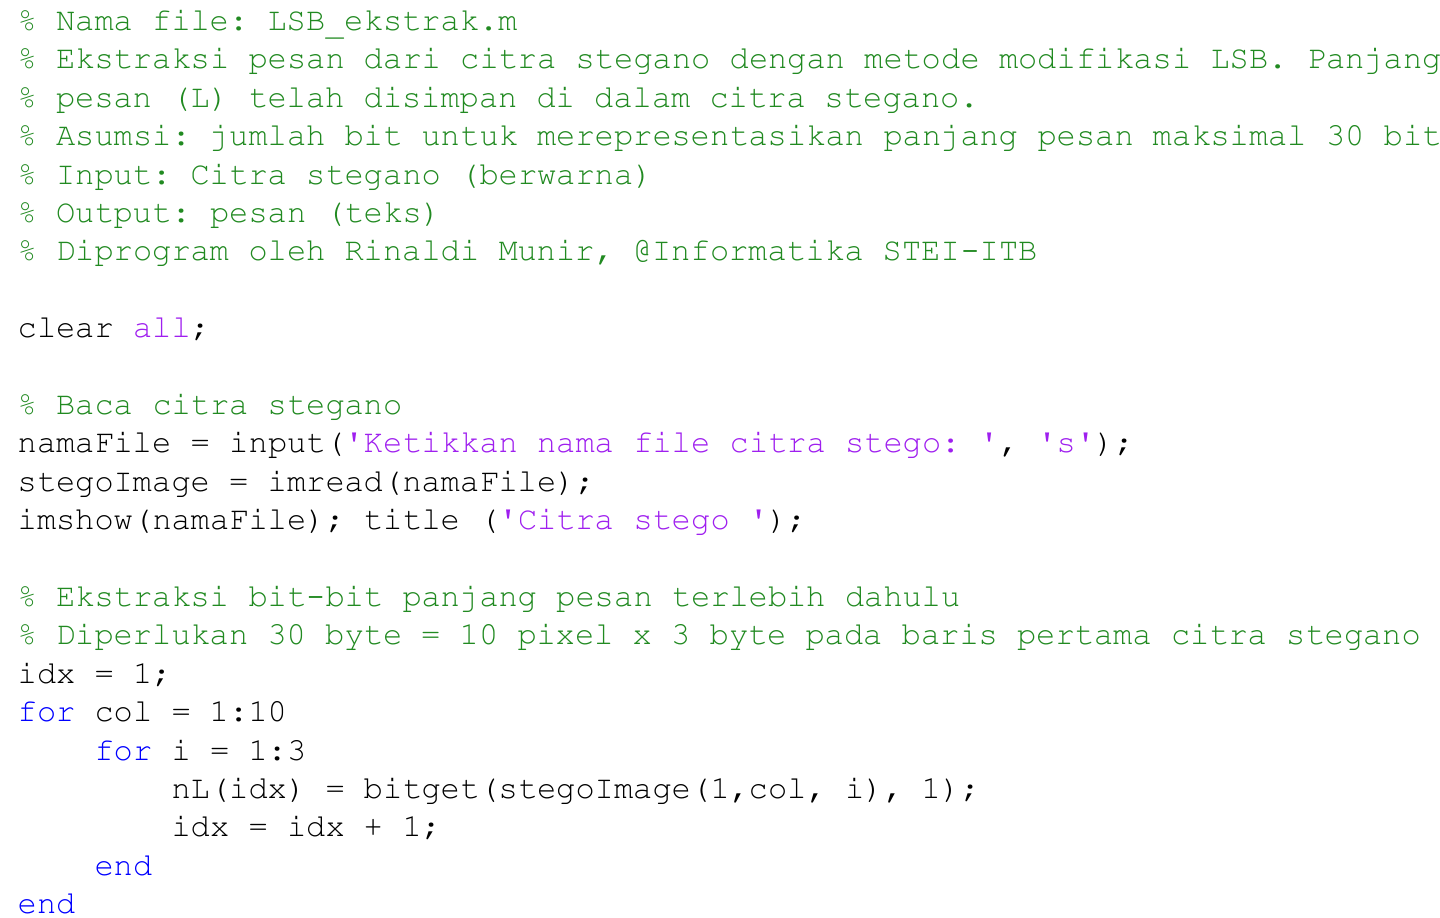
\includegraphics[width=157.50mm,height=252.45mm]{images/llm/page_070_img_01.png}%
\end{textblock*}

\newpage

% --- unit llm 71 ---
% === Halaman 71 (llm) ===

\begin{verbatim}
% Konversi biner ke desimal
L = 0;
for idx = 1:30
    L = L + double(nL(idx))*(2^(30-idx));
end

\vspace{119.39mm}

% Ekstraksi bit-bit pesan ke dalam vektor biner, bit-bit panjang pesan
% ikut dibaca kembali dari awal
m = L*8 + 30; % panjang bit pesan yang harus dibaca
disp('Ekstraksi pesan....');
idx = 1;
for row = 1 : size(stegoImage,1)
    for col = 1 : size(stegoImage,2)
        for i = 1 : 3
            if idx <= m
                vektorBiner(idx) = bitget(stegoImage(row,col, i), 1);
                idx = idx + 1;
            end
        end
    end
end
\end{verbatim}

% deskripsi: Screenshot potongan kode program MATLAB untuk konversi biner ke desimal dan ekstraksi pesan dari stegoImage.
% bbox normalisasi: [0.0600, 0.4200, 0.7830, 0.8220]
\begin{textblock*}{151.83mm}(12.60mm,124.74mm)
\noindent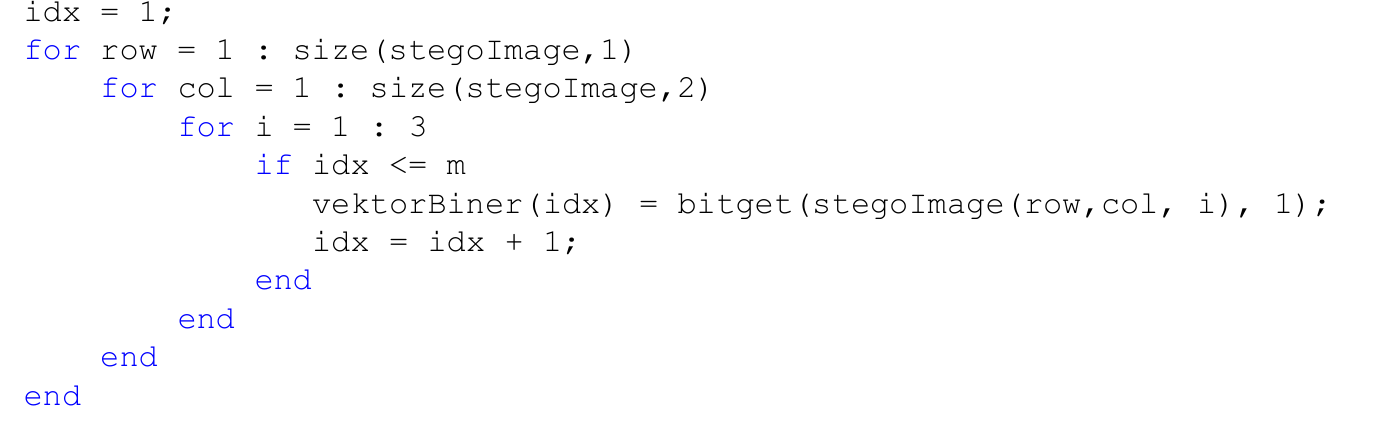
\includegraphics[width=151.83mm,height=119.39mm]{images/llm/page_071_img_01.png}%
\end{textblock*}

\newpage

% --- unit llm 72 ---
% === Halaman 72 (llm) ===

\begin{verbatim}
% Ambil hanya bit-bit pesan
vektorBiner = vektorBiner(31:m);

\vspace{89.10mm}

% Ubah vektor biner ke desimal
for i = 1 : L
    bin(i,:) = vektorBiner((i-1)*8 + 1 : i*8);
    dec(i) = bin2dec(num2str(bin(i,:)));
end
pesan = char(dec);

%Tampilkan pesan
disp('Pesan yang diekstraksi:');
disp(pesan)
\end{verbatim}

\vspace{10mm}

\textbf{Running program:}

\begin{verbatim}
>> LSB_ekstrak
Ketikkan nama file citra stegano: output.bmp
Ekstraksi pesan....
Pesan yang diekstraksi:
Mari kita jaga negara kesatuan Republik Indonesia tercinta. Oke?
\end{verbatim}

% deskripsi: Screenshot jendela MATLAB yang menampilkan gambar paprika warna-warni dengan judul 'Citra stego'.
% bbox normalisasi: [0.5780, 0.2200, 0.9680, 0.5200]
\begin{textblock*}{81.90mm}(121.38mm,65.34mm)
\noindent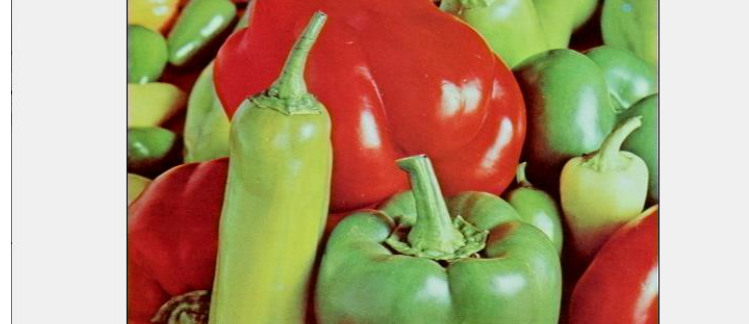
\includegraphics[width=81.90mm,height=89.10mm]{images/llm/page_072_img_01.png}%
\end{textblock*}

\newpage

% --- unit llm 73 ---
% === Halaman 73 (llm) ===

1. Program Steganografi dengan Python

\begin{itemize}
    \item Kode program Python berikut ini menyisipkan pesan dengan metode LSB.
    \item \textbf{A. Program penyisipan pesan}
    \begin{itemize}
        \item Input:
        \begin{enumerate}
            \item Citra berwarna (RGB)
            \item Pesan teks (diketik langsung dari keyboard, atau copas dari file teks)
        \end{enumerate}
        \item Output: citra stego (\textit{stego image})
    \end{itemize}
    \item \textbf{B. Program ekstraksi pesan}
    \begin{itemize}
        \item Input: Citra stego
        \item Output: pesan
    \end{itemize}
\end{itemize}

\newpage

% --- unit llm 74 ---
% === Halaman 74 (llm) ===

\vspace{278.29mm}

\begin{verbatim}
import numpy as np
from PIL import Image

def EmbeddingPesan(cover, pesan, stego):
    # Baca citra cover, ekstrak pixel-pixel sebagai sebuah larik (array)
    citra = Image.open(cover, 'r')
    citra = citra.convert("RGB")
    n = 3
    citra.show()
    lebar, tinggi = citra.size
    larik_pixel = np.array(list(citra.getdata()))

    total_pixel = larik_pixel.size//n    #jumlah pixel di dalam citra
    pesan = pesan + "#####"    #tambahkan delimiter '#####' untuk menandai akhir pesan

    #ubah pesan menjadi string biner
    pesan_biner = ''.join((format(ord(i), "08b") for i in pesan))
    panjang_bit_pesan = len(pesan_biner)

    # periksa apakah jumlah pixel di dalam citra mencukupi untuk menyisipkan pesan
    if panjang_bit_pesan > total_pixel:
        print("ERROR: Ukuran citra tidak mencukupi untuk penyembunyian pesan")
    else:
\end{verbatim}

% deskripsi: Screenshot kode program Python untuk fungsi EmbeddingPesan menggunakan pustaka numpy dan PIL untuk steganografi citra.
% bbox normalisasi: [0.0470, 0.0300, 0.9420, 0.9670]
\begin{textblock*}{187.95mm}(9.87mm,8.91mm)
\noindent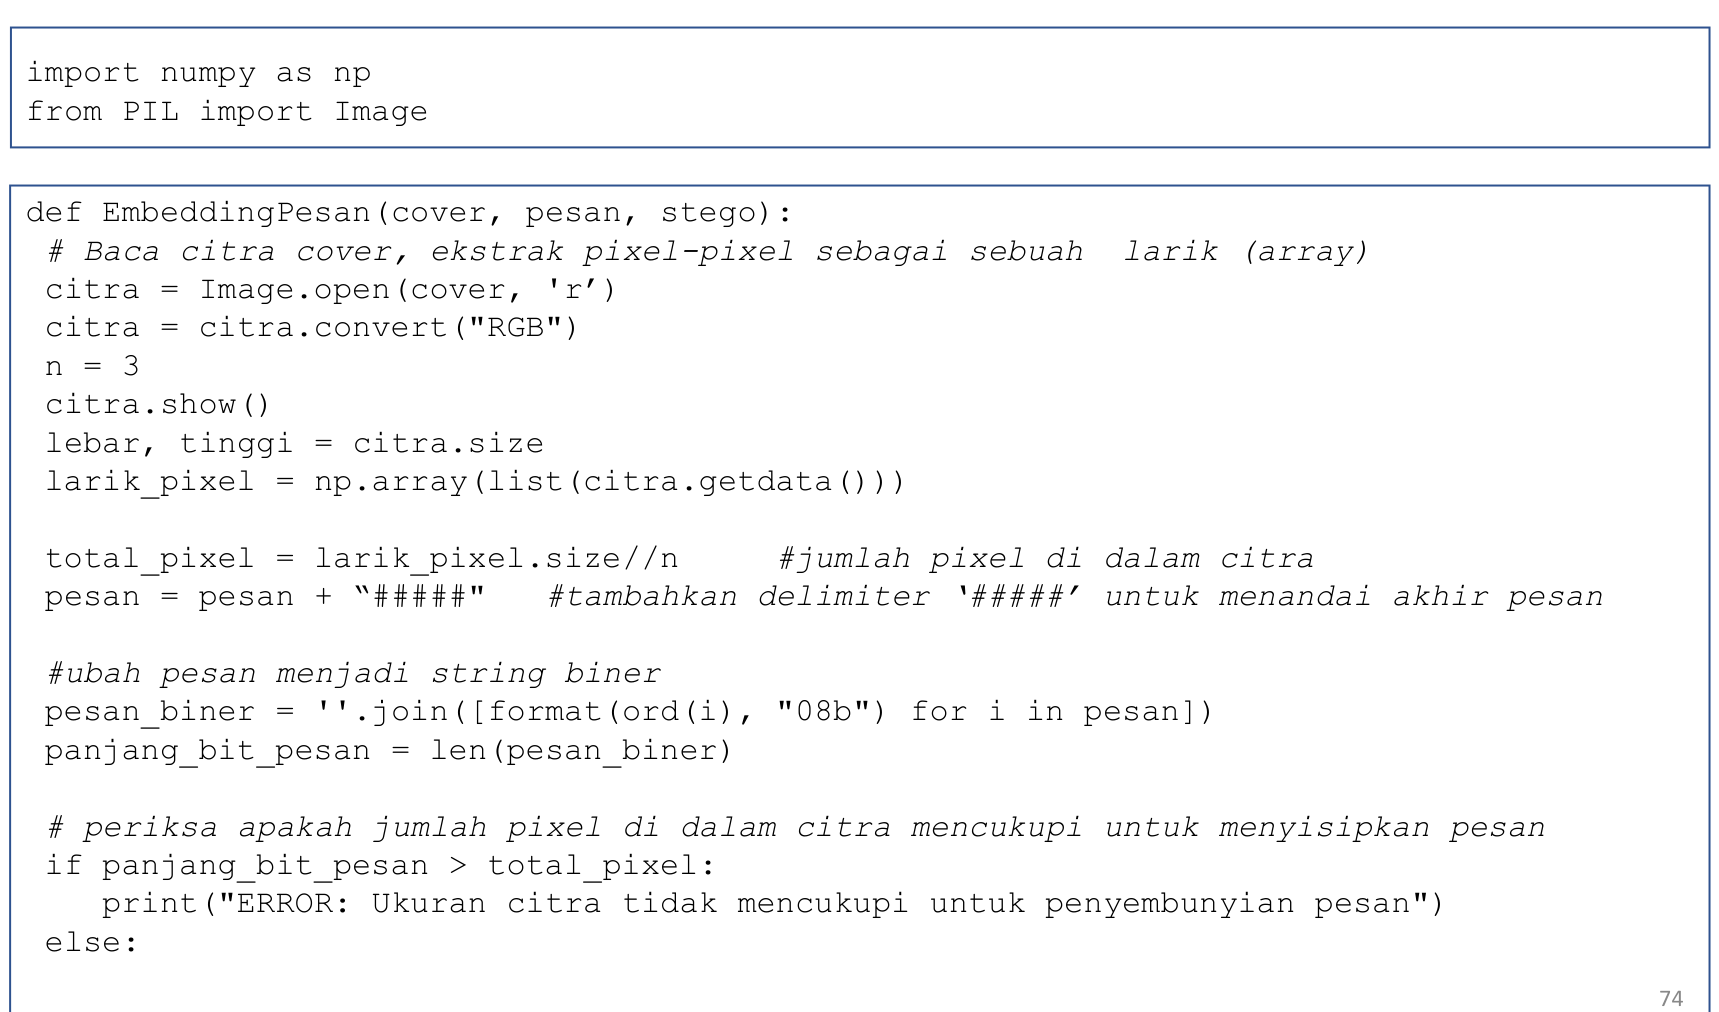
\includegraphics[width=187.95mm,height=278.29mm]{images/llm/page_074_img_01.png}%
\end{textblock*}

\newpage

% --- unit llm 75 ---
% === Halaman 75 (llm) ===

\vspace{154.44mm}

\begin{verbatim}
# Sisipkan bit-bit pesan pada LSB setiap byte
index = 0
for p in range(total_pixel):
    for q in range(3):
        if index < panjang_bit_pesan:
            larik_pixel[p][q] = (larik_pixel[p][q] & 254) | int(pesan_biner[index])
            # 254 = 11111110 dalam biner
            index = index + 1

larik_pixel = larik_pixel.reshape(tinggi, lebar, n)
stego_image = Image.fromarray(larik_pixel.astype('uint8'), citra.mode)
stego_image.save(stego)
print("Penyisipan pesan ke dalam citra berhasil")
\end{verbatim}

% deskripsi: Cuplikan kode pemrograman Python untuk implementasi teknik steganografi Least Significant Bit (LSB).
% bbox normalisasi: [0.0500, 0.1000, 0.9500, 0.6200]
\begin{textblock*}{189.00mm}(10.50mm,29.70mm)
\noindent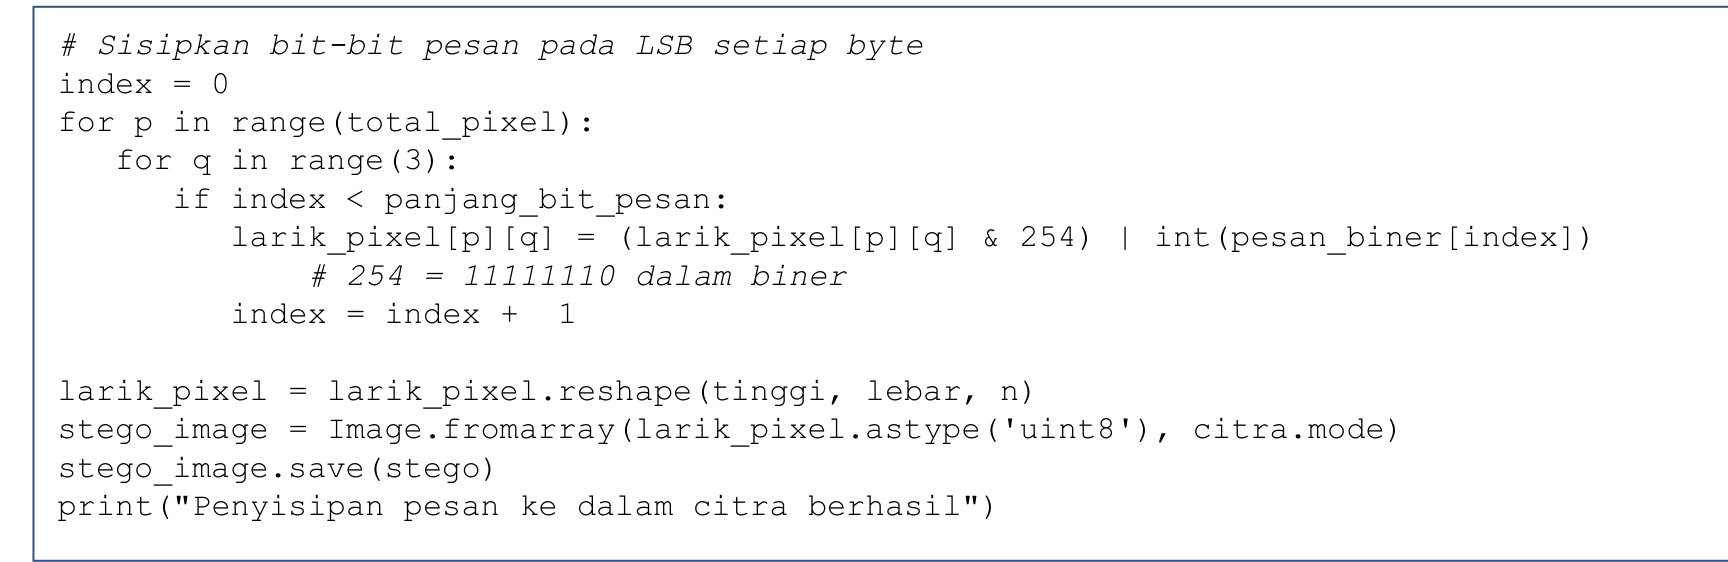
\includegraphics[width=189.00mm,height=154.44mm]{images/llm/page_075_img_01.png}%
\end{textblock*}

\newpage

% --- unit llm 76 ---
% === Halaman 76 (llm) ===

% (tidak ada teks dari model)

% deskripsi: Screenshot kode program Python untuk fungsi EkstraksiPesan yang mengimplementasikan ekstraksi pesan menggunakan metode LSB (Least Significant Bit) dari sebuah citra stego.
% bbox normalisasi: [0.0580, 0.1050, 0.9410, 0.7960]
\begin{textblock*}{185.43mm}(12.18mm,31.18mm)
\noindent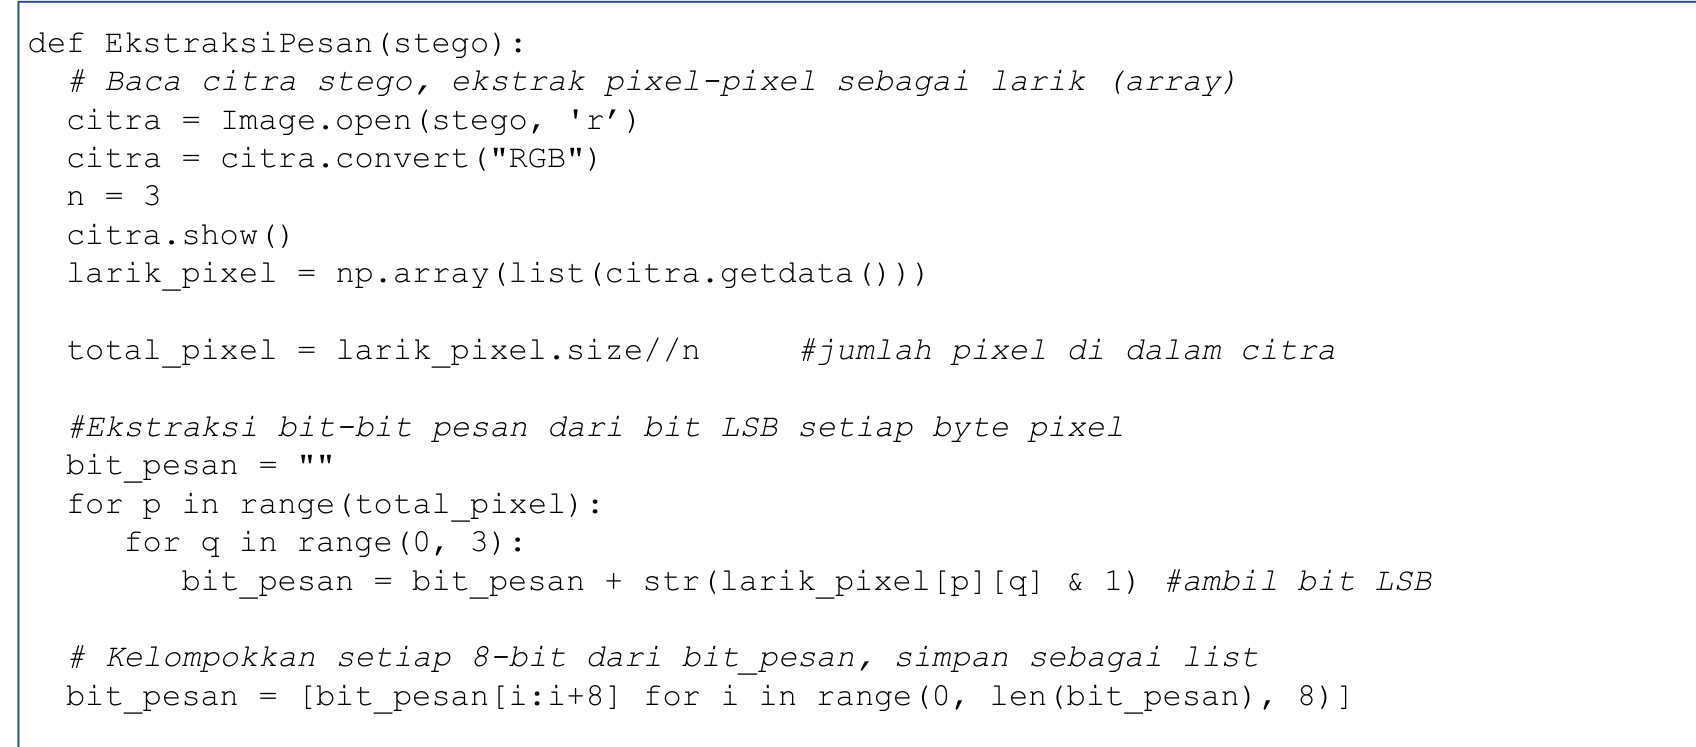
\includegraphics[width=185.43mm,height=205.23mm]{images/llm/page_076_img_01.png}%
\end{textblock*}

\newpage

% --- unit llm 77 ---
% === Halaman 77 (llm) ===

\vspace{148.50mm}

\begin{verbatim}
# Ubah 8-bit pesan ke dalam setiap karakter
pesan = ""
for i in range(len(bit_pesan)):
    if pesan[-5:] == "#####": # ketemu delimiter
        break
    else:
        pesan = pesan + chr(int(bit_pesan[i], 2))

if "#####" in pesan:
    print("Pesan yang diekstraksi:", pesan[:-5])
else:
    print("Tidak ada pesan tersembunyi di dalam citra")
\end{verbatim}

% deskripsi: Screenshot cuplikan kode Python untuk mengekstraksi pesan dari rangkaian bit, dengan pengecekan delimiter '#####'.
% bbox normalisasi: [0.0500, 0.0500, 0.9400, 0.5500]
\begin{textblock*}{186.90mm}(10.50mm,14.85mm)
\noindent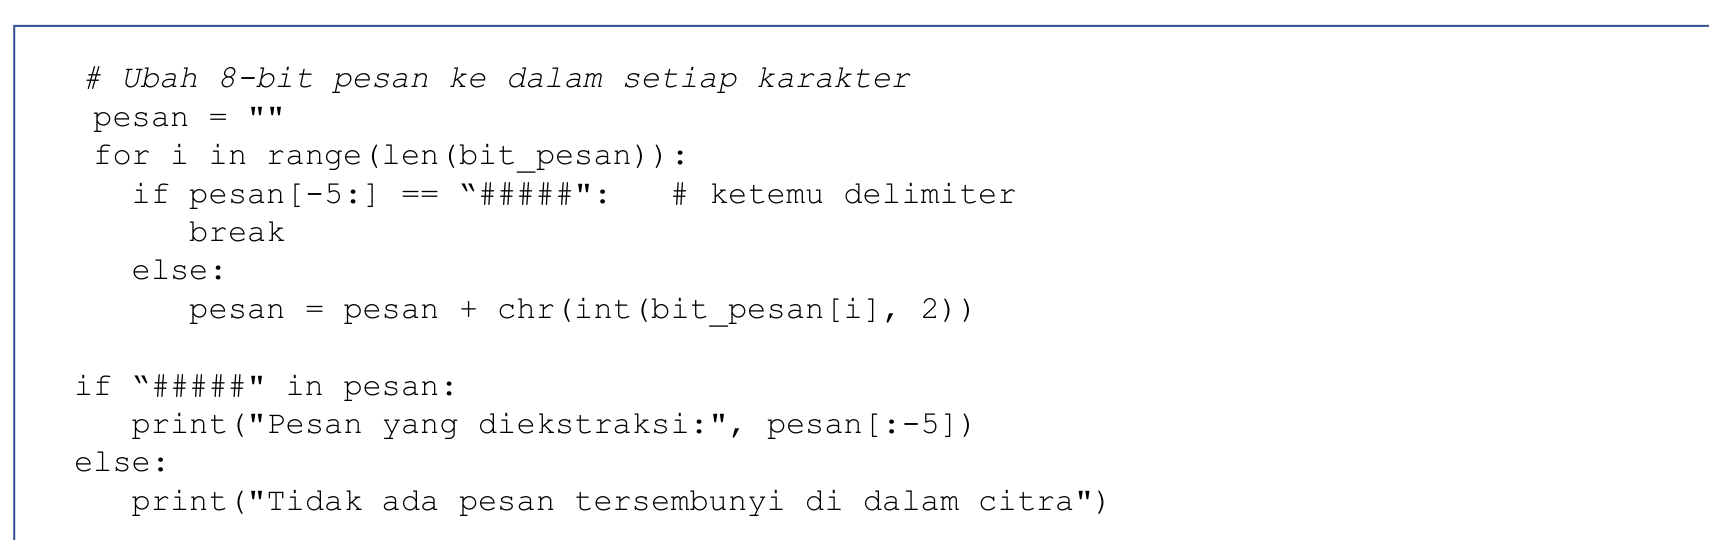
\includegraphics[width=186.90mm,height=148.50mm]{images/llm/page_077_img_01.png}%
\end{textblock*}

\newpage

% --- unit llm 78 ---
% === Halaman 78 (llm) ===

\begin{verbatim}
def ProgramSteganografi():
    print("-- Steganografi pada Citra Digital --")
    print("1: Penyisipan pesan")
    print("2: Ekstraksi pesan")

\vspace{136.62mm}

    pilih = input()
    if pilih == '1':
        print("Masukkan nama citra cover (beserta path-nya")
        cover = input()
        print("Ketikkan pesan yang akan disisipkan ke dalam citra")
        pesan = input()
        print("Masukkan nama citra output (stego image) beserta path-nya")
        stego = input()
        print("Penyisipan pesan...")
        EmbeddingPesan(cover, pesan, stego)
    elif pilih == '2':
        print("Masukkan nama citra stego beserta path-nya")
        stego = input()
        print("Ekstraksi pesan...")
        EkstraksiPesan(stego)
    else:
        print("Pilihan salah")
\end{verbatim}

% deskripsi: Screenshot blok kode Python untuk program steganografi citra digital
% bbox normalisasi: [0.0400, 0.4100, 0.9400, 0.8700]
\begin{textblock*}{189.00mm}(8.40mm,121.77mm)
\noindent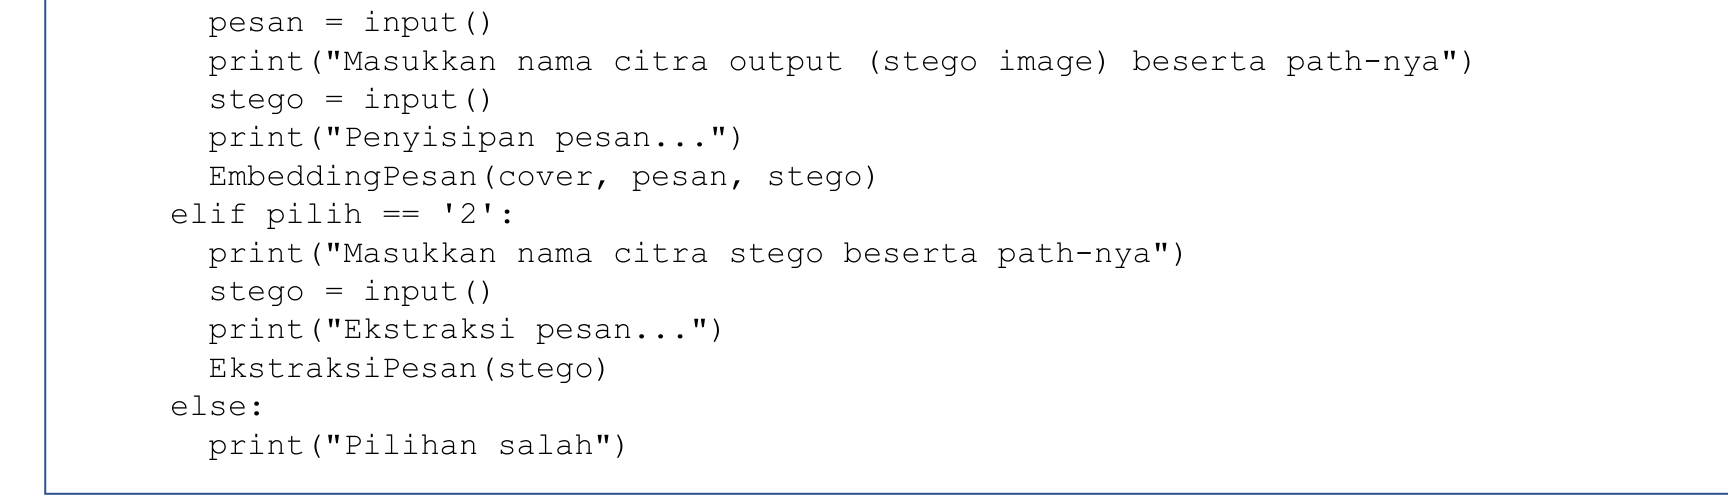
\includegraphics[width=189.00mm,height=136.62mm]{images/llm/page_078_img_01.png}%
\end{textblock*}

\newpage

% --- unit llm 79 ---
% === Halaman 79 (llm) ===

- Steganografi pada Citra Digital --
\begin{enumerate}
  \item Penyisipan pesan
  \item Ekstraksi pesan
\end{enumerate}

Masukkan nama citra cover (beserta path-nya)

E:\\MyWebsite\\Kriptografi-dan-Koding\\2025-2026\\foto2.jpg

Ketikkan pesan yang akan disisipkan ke dalam citra

TEMPO Interaktif, London - Tak selamanya crop circle dibuat manusia. Pada 6 Juli 2009, seorang saksi menyaksikan makhluk asing di lokasi crop circle di Silbury Hill, Wiltshire, Inggris. Wiltshire merupakan wilayah dengan "jejak alien" terbanyak, yang kemunculannya lebih dari 12 titik setiap musim panas. Saksi yang dirahasiakan namanya tersebut adalah petugas kepolisian dengan pangkat sersan. Usai bertugas, dia mendapati tiga sosok berdiri dekat sebuah crop circle. Petugas itu lalu menghentikan kendaraannya dan mendekat. Sosok itu berwujud tiga laki-laki bertinggi sekitar 1,8 meter dengan rambut pirang. Saat didekati terdengar suara seperti listrik statis.

Masukkan nama citra output (stego image) beserta path-nya - harus citra dengan format PNG

E:\\MyWebsite\\Kriptografi-dan-Koding\\2025-2026\\foto2-stego.png

Penyisipan pesan...(tunggu dengan sabar)
Tampilkan citra cover:

\newpage

% --- unit llm 80 ---
% === Halaman 80 (llm) ===

\vspace{264.33mm}

Tampilkan citra cover:\vspace{5mm}

Tampilkan citra stego:

% deskripsi: Citra cover yang menampilkan sekelompok mahasiswa di dalam kelas.
% bbox normalisasi: [0.0500, 0.0900, 0.4300, 0.9800]
\begin{textblock*}{79.80mm}(10.50mm,26.73mm)
\noindent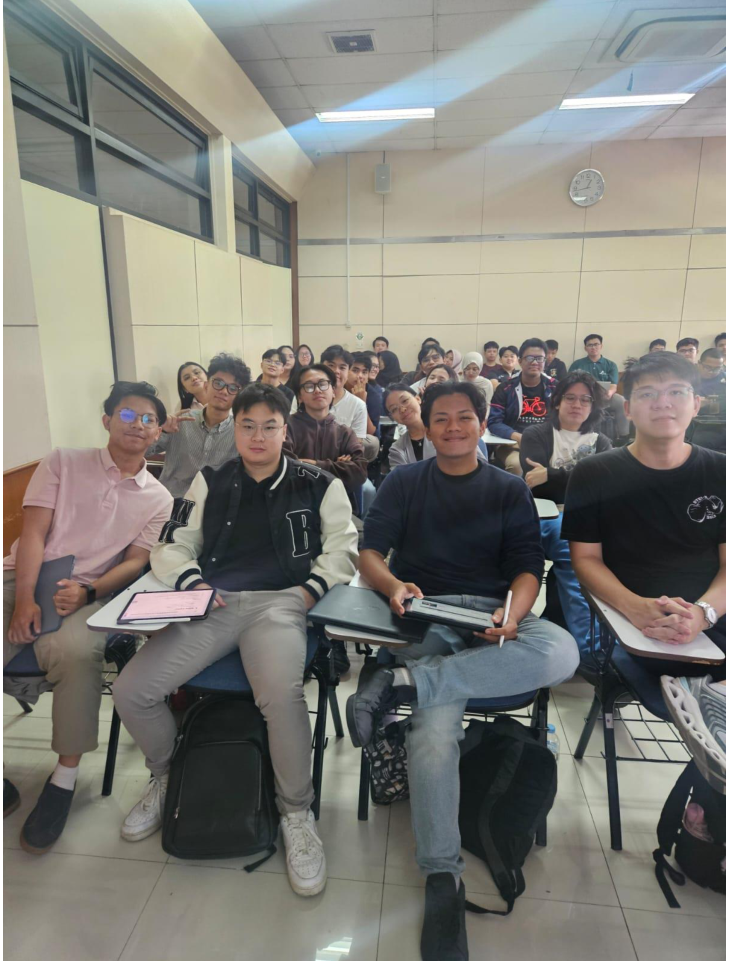
\includegraphics[width=79.80mm,height=264.33mm]{images/llm/page_080_img_01.png}%
\end{textblock*}

% deskripsi: Citra stego yang terlihat identik dengan citra cover, menampilkan sekelompok mahasiswa di dalam kelas.
% bbox normalisasi: [0.5000, 0.0900, 0.8800, 0.9800]
\begin{textblock*}{79.80mm}(105.00mm,26.73mm)
\noindent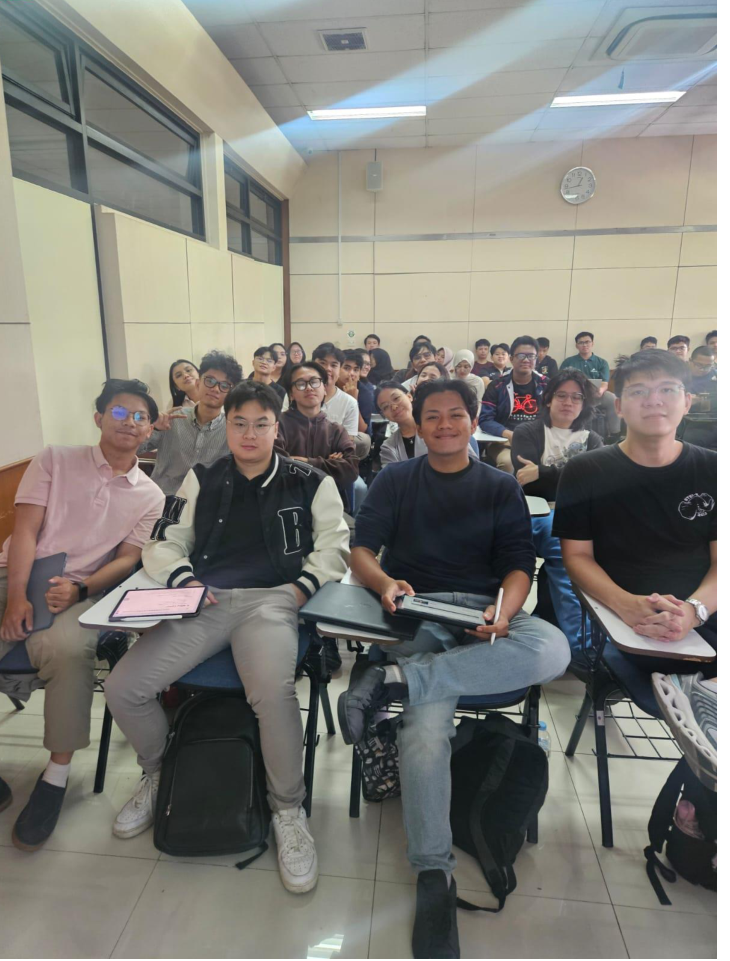
\includegraphics[width=79.80mm,height=264.33mm]{images/llm/page_080_img_02.png}%
\end{textblock*}

\newpage

% --- unit llm 81 ---
% === Halaman 81 (llm) ===

\section*{Latihan}

\begin{itemize}
    \item Kembangkan program di atas sehingga dapat menyembunyikan pesan berupa file sembarang (input pesan berupa file apapun) ke dalam gambar
\end{itemize}

\newpage

% --- unit llm 82 ---
% === Halaman 82 (llm) ===

\section*{2. Program Steganografi Audio dengan Python}

\begin{itemize}
    \item Kode program Python berikut ini menyisipkan pesan dengan metode LSB ke dalam file audio
\end{itemize}

\textbf{A. Program penyisipan pesan}
\begin{itemize}
    \item Input:
    \begin{enumerate}
        \item File audio tidak terkompresi (format WAV)
        \item Pesan (diketik langsung dari keyboard)
    \end{enumerate}
    \item Output: stego audio (format WAV)
\end{itemize}

\textbf{B. Program ekstraksi pesan}
\begin{itemize}
    \item Input: Stego audio (format WAV)
    \item Output: pesan
\end{itemize}

\newpage

% --- unit llm 83 ---
% === Halaman 83 (llm) ===

\vspace{53.46mm}

\section*{Struktur file audio WAV}

\vspace{10mm}

% deskripsi: Diagram struktur format file WAVE yang mencakup deskriptor chunk RIFF, sub-chunk fmt, dan sub-chunk data, lengkap dengan offset file dan ukuran field.
% bbox normalisasi: [0.0200, 0.1200, 0.4200, 0.8900]
\begin{textblock*}{84.00mm}(4.20mm,35.64mm)
\noindent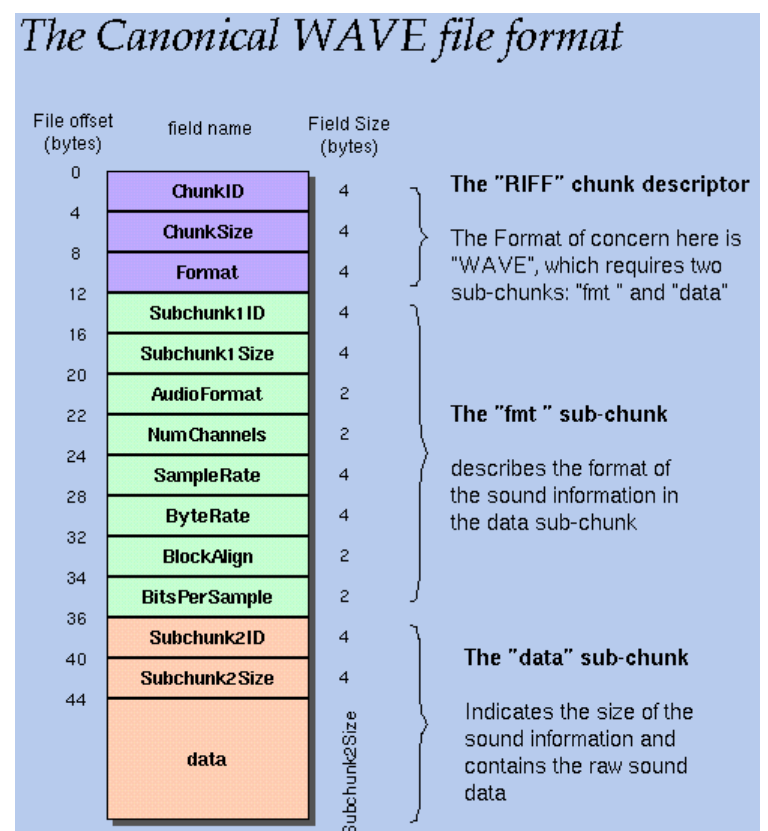
\includegraphics[width=84.00mm,height=228.69mm]{images/llm/page_083_img_01.png}%
\end{textblock*}

% deskripsi: Ilustrasi struktur frame audio WAV yang menunjukkan header (Encoding, Channels, Frame Rate, Bit Depth) dan sampel data audio untuk beberapa frame (Frame #1, Frame #2, Frame #N).
% bbox normalisasi: [0.4400, 0.1200, 0.9900, 0.3000]
\begin{textblock*}{115.50mm}(92.40mm,35.64mm)
\noindent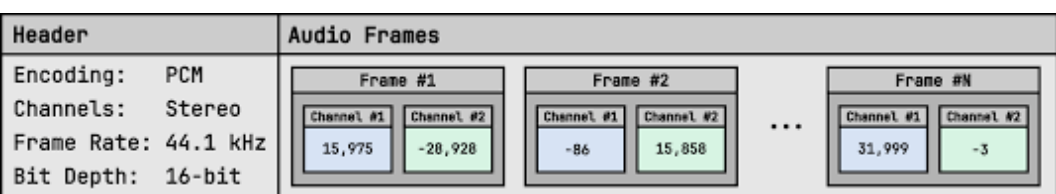
\includegraphics[width=115.50mm,height=53.46mm]{images/llm/page_083_img_02.png}%
\end{textblock*}

\newpage

% --- unit llm 84 ---
% === Halaman 84 (llm) ===

\section*{Struktur Umum File WAV}

\vspace{112.86mm}

Secara berurutan:

\vspace{10mm}

Sumber: ChatGPT

% deskripsi: Diagram struktur hierarki file WAV yang menunjukkan urutan RIFF Header, fmt chunk, data chunk, dan optional chunks.
% bbox normalisasi: [0.0800, 0.3300, 0.9100, 0.7100]
\begin{textblock*}{174.30mm}(16.80mm,98.01mm)
\noindent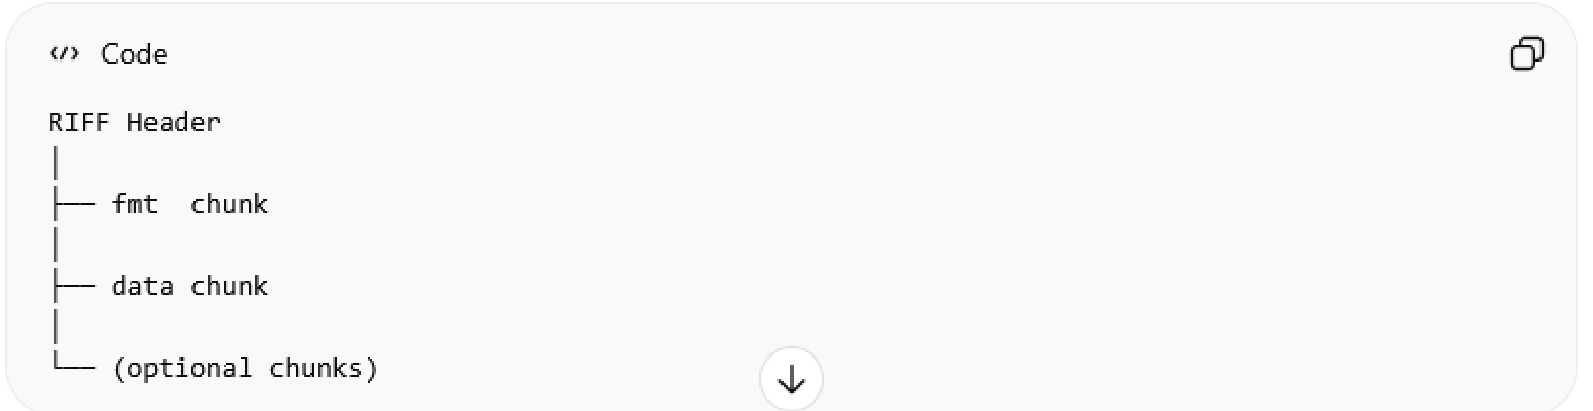
\includegraphics[width=174.30mm,height=112.86mm]{images/llm/page_084_img_01.png}%
\end{textblock*}

\newpage

% --- unit llm 85 ---
% === Halaman 85 (llm) ===

\section*{1 RIFF Header (12 byte pertama)}

\vspace{80.19mm}

Bagian ini adalah identitas file.

\vspace{5mm}

Artinya:
\begin{itemize}
    \item \texttt{''RIFF''} $\rightarrow$ format container
    \item \texttt{''WAVE''} $\rightarrow$ tipe file audio
\end{itemize}

\begin{flushright}
Sumber: ChatGPT
\end{flushright}

% deskripsi: Tabel struktur RIFF Header yang menunjukkan offset, ukuran, dan isi untuk byte 0-11.
% bbox normalisasi: [0.1250, 0.2900, 0.7050, 0.5600]
\begin{textblock*}{121.80mm}(26.25mm,86.13mm)
\noindent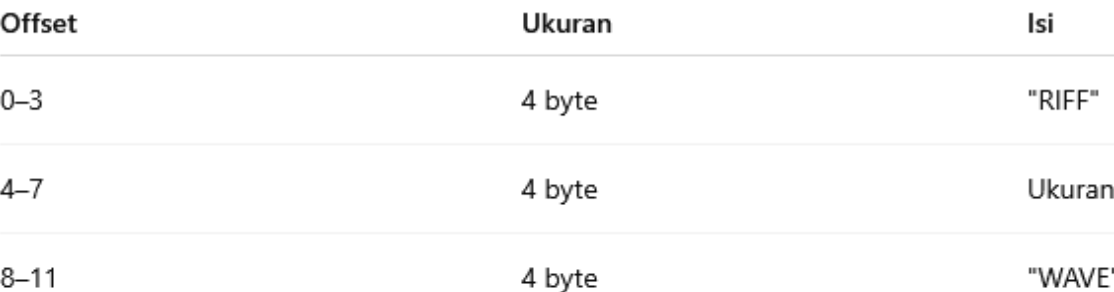
\includegraphics[width=121.80mm,height=80.19mm]{images/llm/page_085_img_01.png}%
\end{textblock*}

\newpage

% --- unit llm 86 ---
% === Halaman 86 (llm) ===

\section*{2 fmt Chunk (Format Chunk)}

Menjelaskan bagaimana audio disimpan.

Struktur:

\begin{tabular}{lll}
\textbf{Field} & \textbf{Ukuran} & \textbf{Keterangan} \\ \hline
"fmt " & 4 byte & ID chunk \\
Subchunk1Size & 4 byte & Biasanya 16 untuk PCM \\
AudioFormat & 2 byte & 1 = PCM \\
NumChannels & 2 byte & 1=Mono, 2=Stereo \\
SampleRate & 4 byte & 44100, 48000, dll \\
ByteRate & 4 byte & $\text{SampleRate} \times \text{NumChannels} \times \text{BitsPerSample}/8$ \\
BlockAlign & 2 byte & $\text{NumChannels} \times \text{BitsPerSample}/8$ \\
BitsPerSample & 2 byte & 16, 24, 32 \\
\end{tabular}

\vspace{20mm}

\begin{flushright}
\textbf{Contoh umum:}
\begin{itemize}
    \item PCM
    \item 2 channel (stereo)
    \item 44100 Hz
    \item 16 bit
\end{itemize}

Sumber: ChatGPT
\end{flushright}

\newpage

% --- unit llm 87 ---
% === Halaman 87 (llm) ===

\section*{3 data Chunk}

Inilah bagian terpenting --- berisi sampel audio mentah.

Struktur:

\begin{tabular}{|l|l|l|}
\hline
\textbf{Field} & \textbf{Ukuran} & \textbf{Keterangan} \\ \hline
"data" & 4 byte & ID chunk \\ \hline
Subchunk2Size & 4 byte & Ukuran data audio \\ \hline
Data & n byte & Sampel audio \\ \hline
\end{tabular}

\vspace{10mm}

\subsection*{Representasi Data Audio}

Misalnya:
\begin{itemize}
    \item 16-bit
    \item Stereo
    \item 44100 Hz
\end{itemize}

Maka struktur sampel:

\begin{center}
\texttt{[L1][R1][L2][R2][L3][R3]...}
\end{center}

Setiap sampel:
\begin{itemize}
    \item 16-bit = 2 byte
    \item Stereo = 4 byte per frame
\end{itemize}

\newpage

% --- unit llm 88 ---
% === Halaman 88 (llm) ===

% (tidak ada teks dari model)

% deskripsi: Screenshot kode program Python untuk fungsi EmbeddingPesan yang mengimplementasikan teknik steganografi pada file audio dengan memodifikasi Least Significant Bit (LSB).
% bbox normalisasi: [0.0300, 0.0400, 0.9700, 0.9600]
\begin{textblock*}{197.40mm}(6.30mm,11.88mm)
\noindent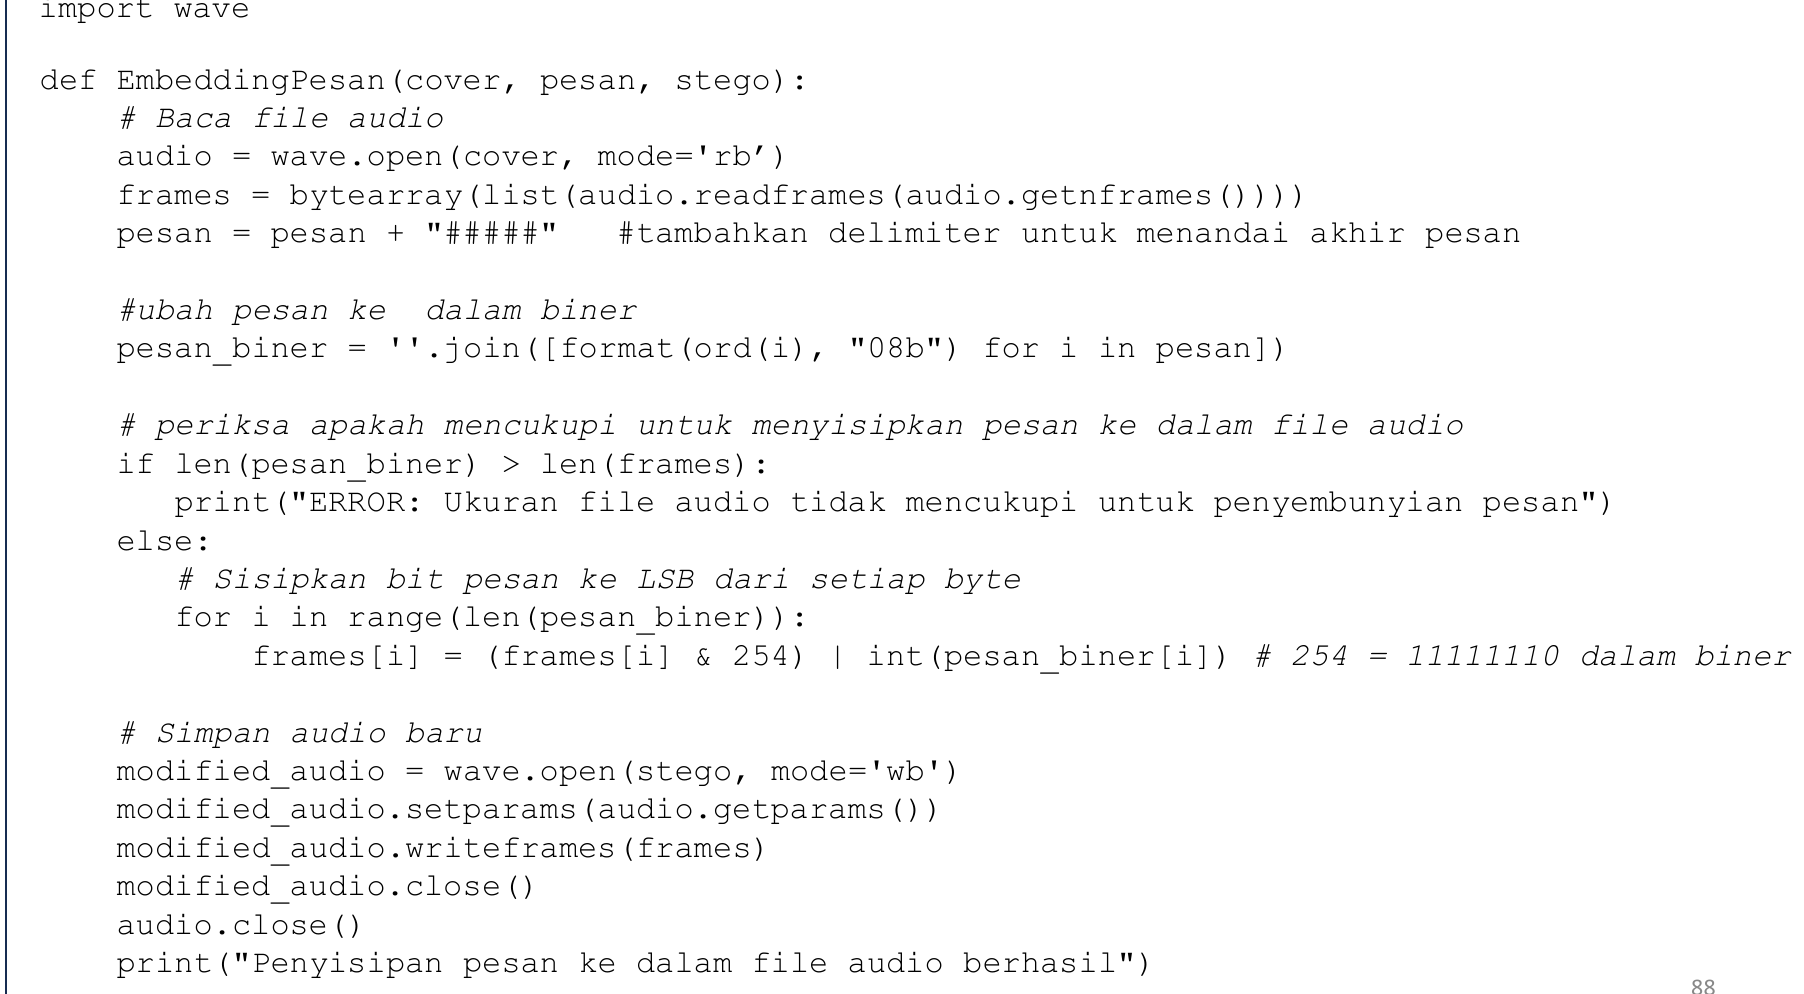
\includegraphics[width=197.40mm,height=273.24mm]{images/llm/page_088_img_01.png}%
\end{textblock*}

\newpage

% --- unit llm 89 ---
% === Halaman 89 (llm) ===

% (tidak ada teks dari model)

% deskripsi: Screenshot cuplikan kode Python fungsi EkstraksiPesan untuk mengambil pesan tersembunyi menggunakan metode LSB pada file audio.
% bbox normalisasi: [0.0400, 0.0100, 0.9600, 0.9800]
\begin{textblock*}{193.20mm}(8.40mm,2.97mm)
\noindent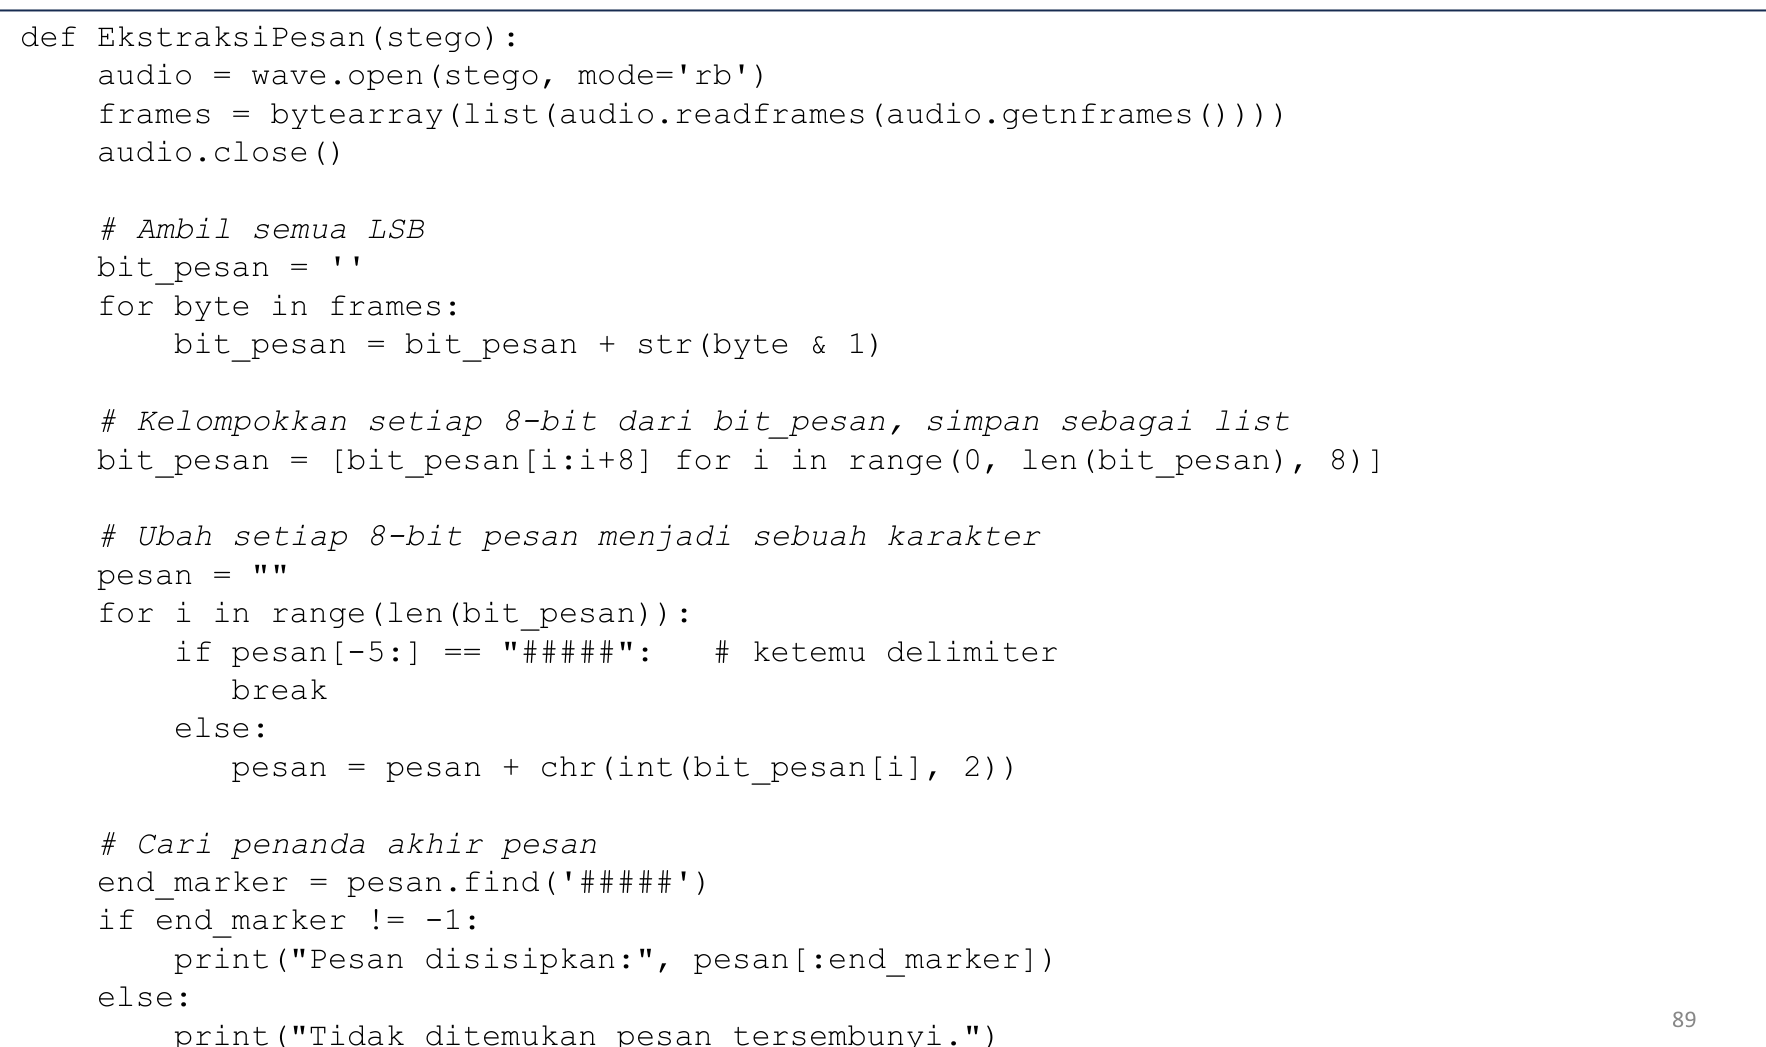
\includegraphics[width=193.20mm,height=288.09mm]{images/llm/page_089_img_01.png}%
\end{textblock*}

\newpage

% --- unit llm 90 ---
% === Halaman 90 (llm) ===

\vspace{255.42mm}

python
def ProgramSteganografiAudio():
    print("-- Steganografi pada file audio WAV --")
    print("1: Penyisipan pesan")
    print("2: Ekstraksi pesan")

    pilih = input()
    if pilih == '1':
        print("Masukkan nama file audio WAV (beserta path-nya)")
        cover = input()
        print("Ketikkan pesan yang akan disisipkan ke dalam citra")
        pesan = input()
        print("Masukkan nama file audio WAV (stego audio) beserta path-nya")
        stego = input()
        print("Penyisipan pesan... (tunggu dengan sabar)")
        EmbeddingPesan(cover, pesan, stego)
    elif pilih == '2':
        print("Masukkan nama file audio stego beserta path-nya")
        stego = input()
        print("Ekstraksi pesan... (tunggu dengan sabar)")
        EkstraksiPesan(stego)
    else:
        print("Pilihan salah")

% deskripsi: Screenshot potongan kode program Python untuk steganografi audio
% bbox normalisasi: [0.0400, 0.0400, 0.9600, 0.9000]
\begin{textblock*}{193.20mm}(8.40mm,11.88mm)
\noindent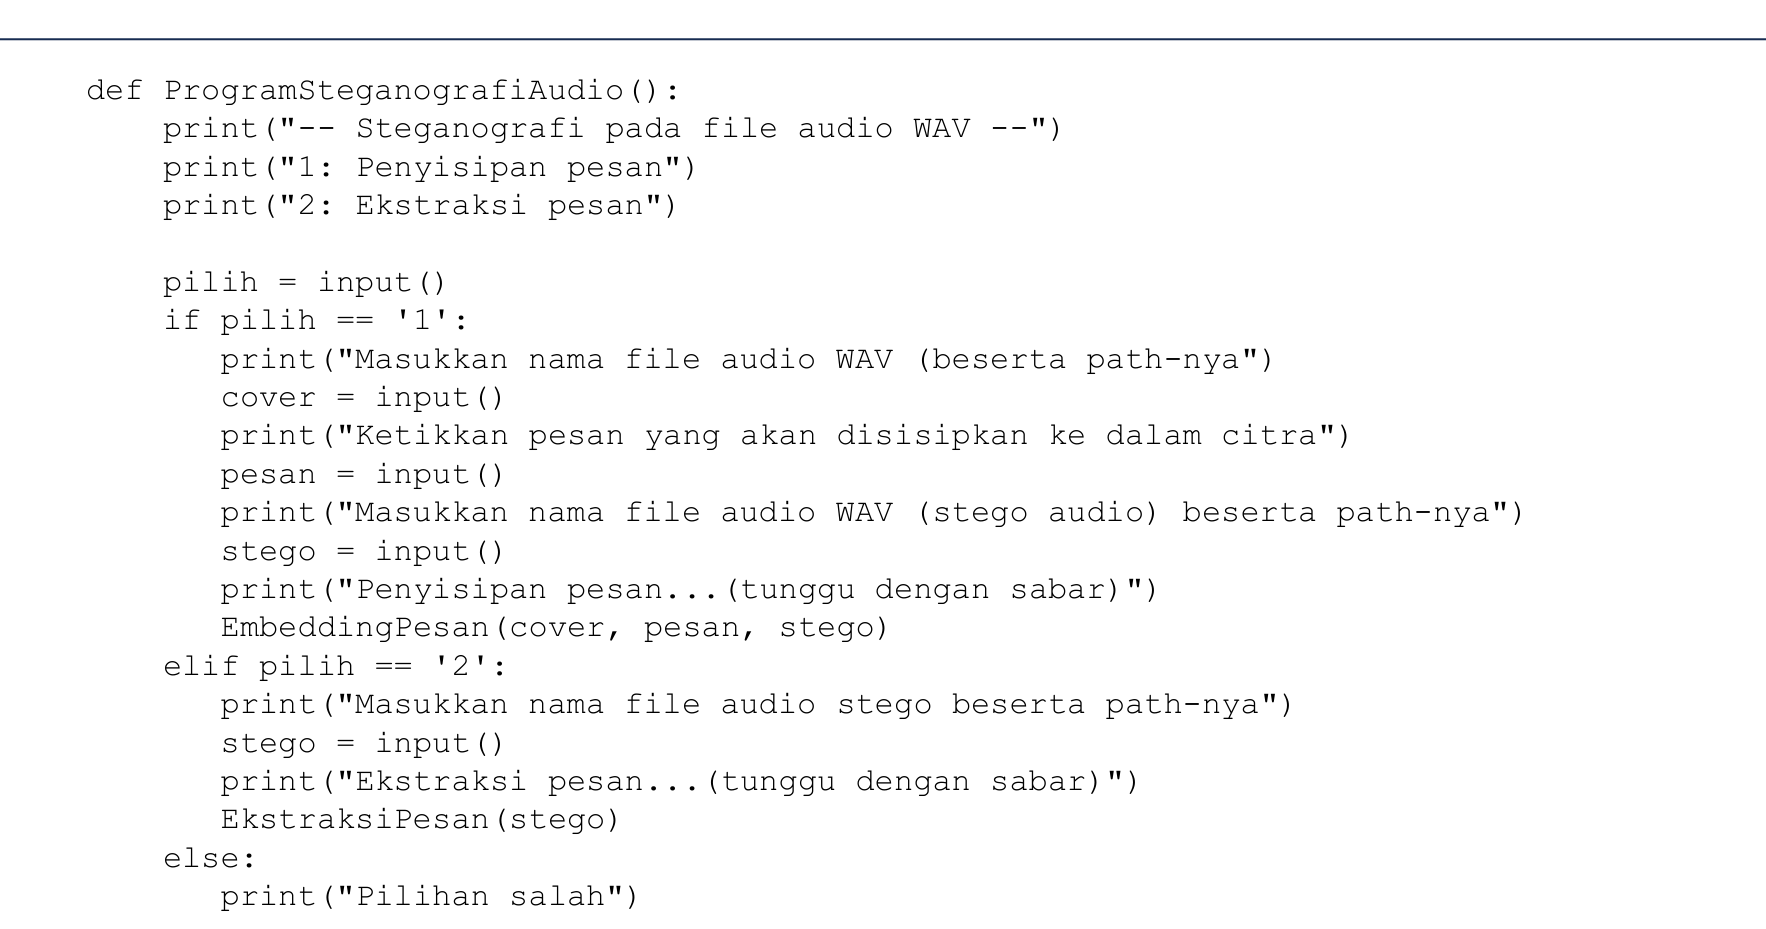
\includegraphics[width=193.20mm,height=255.42mm]{images/llm/page_090_img_01.png}%
\end{textblock*}

\newpage

% --- unit llm 91 ---
% === Halaman 91 (llm) ===

\vspace{134.24mm}

[20]: \texttt{ProgramSteganografiAudio()}

\vspace{10mm}

[34]: \texttt{ProgramSteganografiAudio()}

\vspace{10mm}

% deskripsi: Screenshot output program Python untuk penyisipan pesan (steganografi) ke dalam file audio WAV.
% bbox normalisasi: [0.0600, 0.1020, 0.9410, 0.5540]
\begin{textblock*}{185.01mm}(12.60mm,30.29mm)
\noindent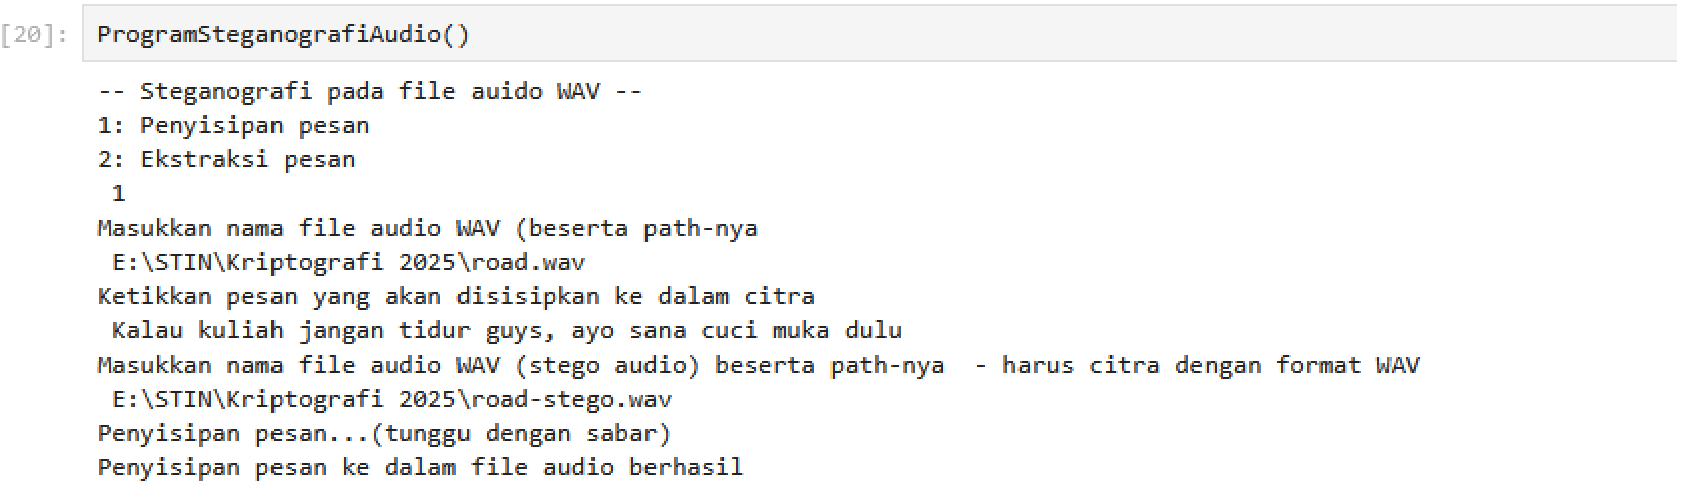
\includegraphics[width=185.01mm,height=134.24mm]{images/llm/page_091_img_01.png}%
\end{textblock*}

% deskripsi: Screenshot output program Python untuk ekstraksi pesan dari file audio stego WAV.
% bbox normalisasi: [0.0600, 0.5840, 0.9410, 0.9010]
\begin{textblock*}{185.01mm}(12.60mm,173.45mm)
\noindent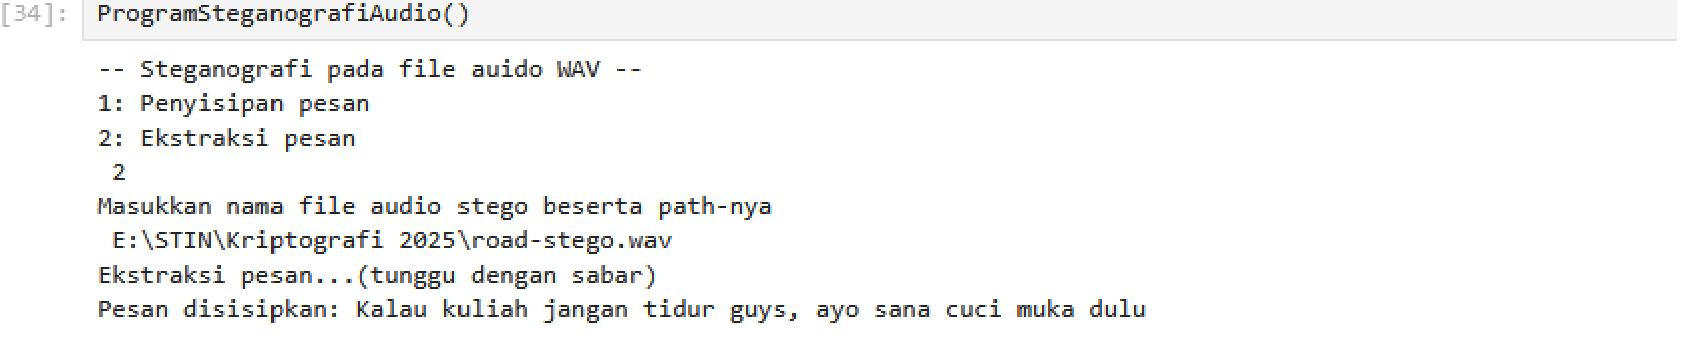
\includegraphics[width=185.01mm,height=94.15mm]{images/llm/page_091_img_02.png}%
\end{textblock*}

\newpage

% --- unit llm 92 ---
% === Halaman 92 (llm) ===

\section*{Catatan:}

\begin{itemize}
    \item Untuk memutar file audio, jika belum terpasang, install terlebih dahulu
    \vspace{5mm}
    \begin{verbatim}
pip install simpleaudio
    \end{verbatim}
    \item Fungsi untuk memutar file audio:
    \vspace{5mm}
    \begin{verbatim}
import simpleaudio as sa

def play_audio(file_path):
    print(f"Memutar audio: {file_path}")
    wave_obj = sa.WaveObject.from_wave_file(file_path)
    play_obj = wave_obj.play()
    play_obj.wait_done() # Tunggu sampai selesai diputar
    \end{verbatim}
\end{itemize}

\newpage

% --- unit llm 93 ---
% === Halaman 93 (llm) ===

\section*{Latihan 2}

\begin{itemize}
    \item Kembangkan program di atas sehingga dapat menyembunyikan pesan berupa file sembarang (input pesan berupa file apapun) ke dalam audio
\end{itemize}

\newpage

% --- unit llm 94 ---
% === Halaman 94 (llm) ===

\section*{Latihan 3}

\begin{itemize}
    \item Buatlah program \textit{hybrid kriptografi} dan steganografi. Mula-mula pesan dienkripsi dengan sebuah cipher (misalnya Vigenere), lalu cipherteks disembunyikan di dalam file gambar atau file audio.
\end{itemize}

\newpage

% --- unit llm 95 ---
% === Halaman 95 (llm) ===

\section*{Referensi}

\begin{itemize}
    \item Li, F., \textit{The art and science of writing hidden messages: Steganography}
    \item Khan, M. M. , \textit{Steganography}
    \item Wohlgemuth, S. (2002), IT-Security: Theory and Practice : \textit{Steganography and Watermarking}, University of Freiburg, Denmakr, 2002.
    \item Tawalbeh, L. (2006), \textit{Watermarking}, Information System Security, AABFS-Jordan.
\end{itemize}

\end{document}
